\pdfoutput=1
\documentclass[10pt,twocolumn]{article}

\usepackage[letterpaper,margin=0.75in,columnsep=0.25in]{geometry}
\usepackage[T1]{fontenc}
\usepackage{amsmath,amsthm}
\usepackage{newtxtext,newtxmath}
\usepackage[numbers,sort&compress]{natbib}
\usepackage{graphicx}
\usepackage{booktabs}
\usepackage{xcolor}
\usepackage{array}
\usepackage[shortlabels]{enumitem}
\usepackage[hidelinks]{hyperref}
\hypersetup{pdftitle={Thrashing Returns: Metastable Failures in Prefix-Cached Agent Serving},pdfauthor={Akshat Valse, Ali Jannesari}}

\setlist{itemsep=1pt,topsep=3pt,parsep=0pt,leftmargin=*}
\renewcommand{\topfraction}{0.85}
\raggedbottom
\makeatletter\setlength{\@fptop}{0pt}\makeatother

\def\UrlBreaks{\do\/\do\-\do\_\do\.}
\renewcommand{\bibfont}{\raggedright}
\newcommand{\fpath}[1]{\nolinkurl{#1}}
\newcommand{\repourl}{\url{https://github.com/AkshatValse/Nova-Research}}

\newcommand{\pending}[1]{\textcolor{red}{[pending: #1]}}

\newcommand{\lmiss}{\lambda_{\mathrm{miss}}}
\newcommand{\lref}{\lambda_{\mathrm{ref}}}
\newcommand{\ledge}{\lambda_{\mathrm{e}}}
\newcommand{\muinf}{\mu_{\infty}}
\newcommand{\Elb}{E_{\mathrm{lb}}}
\newcommand{\Nlb}{N_{\mathrm{lb}}}
\newcommand{\ncap}{n_{\mathrm{cap}}}
\newcommand{\sps}{\,sessions/s}

\newtheorem{proposition}{Proposition}
\theoremstyle{remark}
\newtheorem*{remark}{Remark}

\title{Thrashing Returns: Metastable Failures in Prefix-Cached Agent Serving}
\author{Akshat Valse\thanks{Corresponding author.} \qquad Ali Jannesari\\[2pt]
Department of Computer Science, Iowa State University, Ames, IA, USA\\[2pt]
\texttt{avalse@iastate.edu} \qquad \texttt{jannesar@iastate.edu}}
\date{}

\begin{document}
\maketitle

\begin{abstract}
Prefix caching keeps an LLM agent session's KV across the tool calls between turns, so a turn that hits prefills only its new tokens. We show that this can make the engine's high-hit state metastable. On SGLang 0.5.22 with Qwen2.5-7B-Instruct, one A100 80GB and a 300k-token KV pool, closed-population throughput $\mu(n)$ peaks at 0.233\sps{} at $n=24$ and falls to all-miss by $n=48$, while an empty server stayed good in single 3000\,s runs at nominal rates up to 2.0 times $\lref=0.0715$\sps, the measured all-miss capacity, and was unstable at 2.5. In a pre-registered paired test at 1.35 and 1.65 $\lref$, a burst of 200 sessions trapped the server by the registered rule in 5 of 6 runs, and all 6 had zero cache hits over an evaluation window ending 7500\,s after it; without the burst 6 of 6 stayed good, and a client-side cap of 20 sessions recovered 6 of 6. A simulator whose cost model was fitted only to server-log timing predicted this outcome in a commit pushed before submission. vLLM 0.32.0's own curve and edge give the same window and cap, with a steeper cliff; exploratory burst-only runs had zero hits in 6 of 6, and a registered paired test is pending. With the pool SGLang sizes itself (955,757 tokens) the cliff moves out about threefold, the from-empty edge is between 5.5 and 6.5 $\lref$, and a second pre-registered test at 2.5 and 4.0 $\lref$ with a cap of 64 put all 18 runs in their predicted states. Rates are nominal; runs use one model, one GPU type and synthetic sessions with exponential tool times and no shared prefixes. We give a quasi-static model, prove that under request-level FCFS and stated assumptions no online eviction rule lets $\mu(n)$ exceed the all-miss capacity as $n\to\infty$, compare published mechanisms in an earlier, uncalibrated simulator, and give a diagnostic: measure $\mu(n)$ for the workload and cap sessions from it.
\end{abstract}

\section{Introduction}\label{sec:intro}

\begin{figure*}[t]
\centering
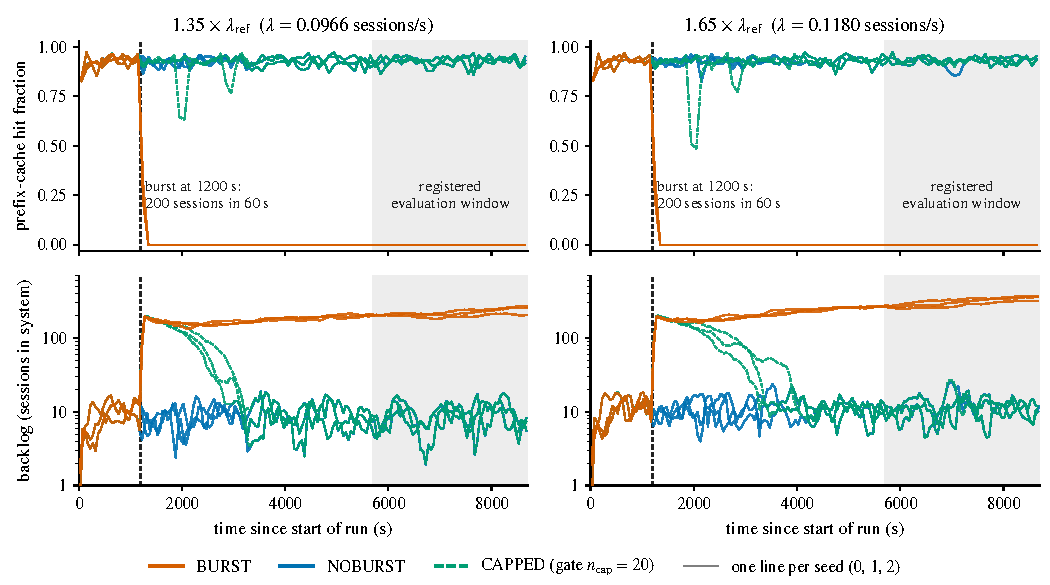
\includegraphics[width=\textwidth]{figs/fig1_e2_timeseries.pdf}
\caption{The registered paired test on SGLang (E2) at nominal rates of 1.35 $\lref$ (left) and 1.65 $\lref$ (right), $\lref=0.0715$\sps; over the evaluation window the three seeds delivered 1.27--1.45 and 1.61--1.75 $\lref$. Top: hit fraction (turns with more than half of the prompt cached) in 100\,s windows. Bottom: sessions in the system (log scale), including those in tool calls. One thin line per seed and arm. Dashed: a burst of 200 sessions at 1200\,s. Shaded: the registered evaluation window. The hit series is recomputed from the request logs and matches the registered per-run value to four decimals.}\label{fig:e2}
\end{figure*}

An LLM agent that uses tools sends its serving engine sessions of many turns. Each turn's prompt is the previous context plus the output of the tool just run, and between turns the session is idle while the tool runs. Prefix caching keeps the key--value (KV) state of the previous turn in GPU memory, so a follow-up turn whose prefix is still cached prefills only its new tokens~\citep{zheng2024sglang}. In our workload a follow-up turn that hits prefills 551 tokens, while a miss prefills the whole prompt, about 10,500 tokens on average; over a session, prefill work with every follow-up hitting is about 16 times smaller than with every turn missing.

We show that this can make the engine's good state, in which almost every follow-up turn hits, \emph{metastable}. Let $\lmiss$ be the all-miss capacity, the session throughput of a saturated engine when every turn misses, and $\lref$ its estimate from saturated runs with caching disabled (0.0715\sps{} on SGLang with a 300,000-token KV pool). In our measurements an empty server carried nominal arrival rates between 1.25 and 2 times its own $\lref$ for 3000\,s with 91--93\% of turns hitting, on SGLang and on vLLM with that pool, and up to 5.5 times $\lref$ when SGLang sized its own KV pool. Each rate is a single run with one arrival realization, whose realized rates were 6--13\% above nominal, except that on SGLang with the 300k pool three fresh arrival seeds were run at 2.0 and 2.5 $\lref$ and all stayed good, although the original seed had been unstable at 2.5; ordered by realized arrival rate, the 12 runs put that pool's edge between 2.67 and 2.73 $\lref$ (\S\ref{sec:edge}). A transient burst admits more sessions than the KV pool can hold once their contexts grow. A session with no running request, whether in a tool call or waiting in the queue, holds no lock on its KV, so admitting waiting work evicts it, oldest first; when its next turn is admitted it misses, the miss costs an order of magnitude more prefill, the queue grows, the gap between a session's turns grows with it, and more idle KV is evicted before its owner returns. Every turn then pays a full prefill, and the backlog does not drain (Fig.~\ref{fig:e2}).

Neither the collapse nor the loop that sustains it is new. Throughput that collapses when the working sets of the admitted jobs exceed memory is Denning's thrashing~\citep{denning1968thrashing,denning1968working}, and a bad state that a feedback loop sustains after its trigger is gone is a metastable failure~\citep{bronson2021metastable,huang2022metastable}. That KV left idle during tool calls is evicted and costly to recompute motivates Continuum, InferCept, MORI and TokenCake~\citep{li2025continuum,abhyankar2024infercept,xia2026mori,bian2025tokencake}, and Sutradhara observes, under Poisson load on vLLM, that prefix hit rates collapse despite context reuse, and attributes this to LRU eviction (as in vLLM and SGLang) of the contexts of requests waiting on tool calls~\citep{biswas2026sutradhara}; ThunderAgent and NVIDIA Dynamo treat agents' KV eviction and re-prefill as working-set thrashing~\citep{kang2026thunderagent,dhanani2026dynamo}, and EfficientAgent applies Denning's working-set principle and load control to the host KV tier of a fixed pool of agents~\citep{shao2026efficientagent}. The loop between eviction, cold prefill and queueing is published for closed or bounded populations: for RL rollouts under a concurrency ceiling, MISA-T reports vLLM Router's prefix-cache hit rate falling from 92.4\% to 4.5\%, describes the loop and interrupts it with a session cap~\citep{hong2026misat}; CONCUR halves its window of active agents when the hit rate falls below 0.2 while KV usage exceeds 0.5~\citep{chen2026concur}; Yuan et al.\ and VAMP measure the collapse on vLLM~\citep{yuan2026agentic,kim2026vamp}; and AgentKV, known to us from its abstract, predicts its onset at high concurrency from available KV capacity over per-instance context demand~\citep{anon2026agentkv}. Under open Poisson arrivals on vLLM, KAIROS reports thrashing when its controller lowers the GPU clock or when the arrival rate rises, and, in one run without its thrashing avoidance, a persistent thrashing regime at an arrival rate that a baseline at the maximum clock carries; that run shows no frequency trace, so whether its trigger was removed is not reported, and it has no burst trigger, no fixed clock, no replication and no matched arms~\citep{yuan2026kairos}. What we add is a controlled, replicated test at a fixed clock and pool, two persistent states at one capacity and one arrival rate, entered by a transient burst and checked against matched no-burst and capped arms on common random numbers, and a first-principles account of the thrashing curve in which the hit rate feeds back on itself through the service time and the KV held by running requests, and in which, on the memory-gated all-miss branch, the queue rather than the tool time sets the gap between a session's turns.

Under the default FCFS ordering, our model and simulator predict that a server that passes steady-state load tests at a rate above $\lmiss$ at which it stays good from empty is one sufficiently large burst away from a collapse that, once deep, it does not leave unless the arrival rate falls below $\lmiss$ or admission is bounded. On the engine we have tested two rates per pool with a burst of 200 sessions and, in the registered test B1 at 1.65 $\lref$ on the 300k pool, bursts of 25 and 100: 25 left the engine good and 100 trapped it, in 3 of 3 seeds each, so the good state has a finite basin whose boundary lies between 25 and 100 sessions (\S\ref{sec:frozen}). Registered tests of burst sizes in between, of a cap engaged inside an established trap, of a pause in arrivals and of a temporary slowdown of tool calls are listed there with their frozen predictions, and their outcomes are pending in this version. In our earlier simulator, TTL pins with their pinned-first order, under the preview's release rule, and a pure resident-first order (LPM without SGLang's 128-request fallback) raise the rate below which the system recovers (\S\ref{sec:mech}). On the engine, stock LPM recovered from a 200-session burst at 1.35 $\lref$ in 4 of 6 exploratory runs but in only 1 of 6 at 1.65 (\S\ref{sec:grid}); on our reading of its source, it stops re-sorting its queue when more than 128 requests wait, so in deep congestion Proposition~\ref{prop:A} applies to it as well. With that fallback disabled, in an exploratory run at 1.65 $\lref$, LPM did not collapse on the two arrival streams on which stock LPM had collapsed in 4 of 4 runs, but no run recovered by the registered rule (\S\ref{sec:mech}).

\paragraph{Claims.} Each item says what is ours and what is not; \S\ref{sec:related} gives the full positioning.
\begin{itemize}
\item \textbf{Registered open-system metastability on two engines} (\S\ref{sec:e2}--\ref{sec:vllm}). At a clock, pool and Poisson arrival rate that the engine carried in the good state for the full 8700\,s of every no-burst run, a burst of 200 sessions within 60\,s left it at zero hits, with a backlog that did not drain, to the end of the run, 7500\,s later, and a client-side cap at the peak of $\mu(n)$ drained the same burst. In two pre-registered SGLang tests (pools of 300,000 and 955,757 tokens) BURST was at zero hits in 12 of 12 runs and trapped by the registered rule in 11, NOBURST was good in 12 of 12 and CAPPED recovered in 12 of 12; on vLLM 0.32.0 the registered analysis of a third test passes at both rates, but the frozen decision rule for its mechanism checks is not met, because its online detector also alarmed, during the drain, in two capped runs (\S\ref{sec:vllm}). The loop was published for closed populations, and KAIROS reports a persistent thrashing regime under open arrivals in one uncontrolled run whose clock during the thrashing is not reported~\citep{yuan2026kairos}; ours is a controlled, replicated test at a fixed clock and pool, with a burst trigger and the trigger-and-control design of Huang et al.~\citep{huang2022metastable}: two persistent states at one capacity and offered load, against matched no-burst and capped arms on common random numbers, on two pools and two engines.
\item \textbf{The sustaining variable} (\S\ref{sec:mechanism}). At the same load, the ratio of the reuse gap to the pool's turnover time $R_M=M/\text{churn}$, the time in which the pool is rewritten, is 0.010--0.028 in every good-state run and 4.1--9.7 in every BURST run, on both engines and both pools; turn latency, not tool time, carries the gap past $R_M$, and the trapped value obeys a cost-model-free identity (Proposition~\ref{prop:trapid}). The miss criterion is Denning's and Che's~\citep{denning1968working,che2002hierarchical}, that queueing behind other agents lengthens the gap between an agent's turns has been measured for the host KV tier of a closed pool of agents, whose backlogged-pool working-set scale is the cycle argument behind the identity (EfficientAgent~\citep{shao2026efficientagent}), and the trap is an instance of what Huang et al.\ call capacity-degradation amplification; ours are the measurement in both states at one load and the identity's exact time-domain form on the all-miss FCFS branch, checked against the trapped runs with nothing fitted.
\item \textbf{A first-principles thrashing curve} (\S\ref{sec:fp}). We derive $\mu(n)$ from the pool size, the workload and an iteration-cost model fitted only to server-log timing, with no parameter fitted to any $\mu(n)$, hit or trap measurement (the H200 and vLLM cells take one speed factor fitted to their all-miss token rate), and prove, for the deterministic model, a closed-form all-miss onset (the sessions in tool calls plus one pool of running sessions), a speed law (a faster GPU moves the onset out and lowers the peak ratio $\mu^*/\lmiss$), a fold criterion (a proof sketch) and the trapped identity. The model reproduces the two SGLang curves and misses vLLM's earlier cliff. Metastability from a unimodal throughput curve and its cure by bounded admission are classical~\citep{kleinrock1975aloha,carleial1975bistable,courtois1975decomposability,nelson1987stochastic}, with the slowdown given as a function of occupancy; ours are the derivation of the curve and its closed forms.
\item \textbf{Frozen out-of-sample predictions} (\S\ref{sec:frozen}). Before their results were read by the agents that derived the model, we froze its predictions for an H200 at the same pool, for pools of 150,000 and 600,000 tokens, for Llama-3.1-8B, for a registered dose-response of the probability of a stuck run against burst size (critical fresh burst 53.4 sessions at 1.65 $\lref$) and for a registered rescue in which a cap engaged inside an established trap drains it and the good state persists after release. For the H200 the model predicted a peak ratio of 1.92 at $n\approx32.5$ (against 3.27 predicted and 3.15 measured on the A100), a 0.5-hit crossing at 37.3 sessions and a from-empty edge at 1.39 $\lref$; the engine gave 1.89 at $n=32$ (turns-based; 1.99 in completed sessions), a crossing near 38.9 and, on the original seed-0 runs, an edge in $[1.3,1.4)\,\lref$ (on reseeding, 1.4 $\lref$ was stable in seeds 1 and 2). Past the crossing the measured hit fraction fell gradually, to 0.46 at $n=40$ (0.27 predicted), 0.32 at 44 and 0.16 at 52, where the model is all-miss beyond its onset at 41.3 sessions, so the predicted onset came early; we have not traced this miss to a specific assumption (\S\ref{sec:fp-weak}). The first author, though not those agents, had seen the H200 closed-curve values for $n\le32$, which include the peak, so the H200 peak ratio is not blind to him. The registered basin test B1 passed as predicted: the model gave this exact outcome probability 0.879 (its 100-session predictions blind by access only, since those runs had ended before the push), and the simulator's calls matched all 6 of its runs and all 6 runs of a fresh-seed from-empty test, which did not replicate the first seed's edge (\S\ref{sec:frozen}). The other outcomes are pending in this version. That trap probability depends on the size of the trigger is part of metastability theory~\citep{bronson2021metastable,huang2022metastable,isaacs2025analyzing}; ours is a boundary on an LLM engine predicted before it is measured.
\item \textbf{An ordering bound} (\S\ref{sec:props}). Under request-level FCFS and the assumptions of \S\ref{sec:props}, no online eviction rule, queued-prefix protection and FCFS-order TTL pins included, lets $\mu(n)$ exceed the all-miss capacity as $n\to\infty$ if the congested engine computes prompt tokens no faster than with caching disabled; stock SGLang LPM falls under it in deep congestion through its 128-request fallback. The prefill-saturation bound is MISA-T's~\citep{hong2026misat}, and that arrival-order service sustains metastability is known~\citep{bronson2021metastable,farahbakhsh2026characterizing}; ours is that request-level FCFS drives reuse to zero in congestion whatever the online eviction rule, so that the bound becomes the all-miss capacity.
\item \textbf{A pre-deployment procedure, evaluated} (\S\ref{sec:diag}). Measure $\lmiss$ with the cache off, $\mu(n)$ across the cliff and the from-empty edge; cap admitted sessions at the smallest $n$ within 5\% of the peak, inside the interval $(n_1,n_2)$ of Corollary~\ref{cor:rescue}; re-measure for each workload, pool, engine and GPU. Multiprogramming-level selection, session-based admission, client-side concurrency limits and hit-rate thrashing signals are prior art~\citep{denning1976optimal,cherkasova2002session,maurer2015fail,chen2026concur,hong2026misat}; ours are the evaluation and the placement condition.
\end{itemize}
Registrations committed before their runs, with GitHub's push log as the external record of when each became public, and predictions frozen under pushed tags are how we tried to make these claims checkable. They are rigor, not a contribution; Appendices~\ref{app:prereg} and~\ref{app:timeline} list every registration and prediction round, with the slips in them.

The registered tests use one model, Qwen2.5-7B-Instruct, one GPU type, the A100 80GB, and synthetic sessions with exponential 5\,s tool times and no shared prefixes; on an H200 at the same pool the window narrowed from $(1,2.0)$ to $(1,1.3)$ times that GPU's own $\lref$, too narrow for our registration rule to place its two test points, so that cell is a measurement, not a registered test, and the Llama-3.1-8B cell of \S\ref{sec:frozen}, whose outcome is pending, extends the first. The vLLM registration was committed before its jobs were submitted but reached GitHub only after the first two had started, so we call that test registered, not pre-registered, and its BURST arm reuses the seeds of earlier exploratory vLLM runs (\S\ref{sec:vllm}).

\section{Background and what is classical}\label{sec:background}

\paragraph{Engines.}
LLM engines batch per model iteration: running requests decode one token per iteration and waiting requests join between iterations~\citep{yu2022orca}; KV is stored in pages~\citep{kwon2023vllm}. SGLang keeps cached prefixes in a radix tree, evicts least-recently-used (LRU) leaves, and can order waiting requests by longest prefix match (LPM)~\citep{zheng2024sglang}. In SGLang 0.5.22 the default policy is FCFS and the default eviction rule LRU; LPM stops sorting its queue when more than 128 requests wait, a fallback that PEEK also documents, running its heavy-load cells at that depth~\citep{xie2026peek}; a waiting request does not lock its cached prefix, which is locked when the request is admitted; and under FCFS, including LPM above that threshold, an LRU refresh touches the prefixes of the first 128 waiting requests once every 32 scheduling passes (files under \fpath{python/sglang/srt/} at tag v0.5.22: \fpath{arg_groups/fields/schedule.py}, lines 82--98; \fpath{arg_groups/fields/memory.py}, lines 25--42; \fpath{managers/schedule_policy.py}, lines 133--135, 278--311 and 1591; \fpath{mem_cache/radix_cache.py}, lines 552--580; \fpath{environ.py}, line 594). vLLM 0.32.0 schedules FCFS, its default, or by priority, and a freed cached block keeps its hash until it is reallocated (\fpath{vllm/config/scheduler.py}, lines 21 and 159; \fpath{vllm/v1/core/block_pool.py}, lines 666--690 and 774--803; at tag v0.32.0). We first read these sources through a web tool that returns a language model's summary of each file (Appendix~\ref{app:prov}); the line references here and in Appendix~\ref{app:proofs} are to the files at the tags, read verbatim. Our synthesis of these rules is that in both engines a session's KV is protected only while one of its requests runs.

\paragraph{Thrashing and metastability.}
Denning showed that admitting one more program to a memory near saturation can collapse efficiency, and that keeping the working sets of the active programs within memory, which limits their number, prevents it~\citep{denning1968thrashing,denning1968working}. We call throughput as a function of the closed population $n$ the thrashing curve; the term is our framing. LRU does badly on loops larger than the cache~\citep{chou1985evaluation,smaragdakis1999eelru}. A metastable failure is a bad state that persists after its trigger is removed, sustained by a feedback loop under uncontrolled load; one of Bronson et al.'s case studies is a lost look-aside cache~\citep{bronson2021metastable}, and Huang et al.\ study such failures in production incidents and model them~\citep{huang2022metastable}. In their classification of sustaining effects, a trap in which the load itself lowers capacity is capacity-degradation amplification; one of their cases is garbage collection driven by queueing-induced memory pressure, and their experiments vary the trigger's magnitude against matched runs, the design we follow. In Bronson et al.'s terms, a system that serves its load but can be pushed by a trigger into the bad state is in a vulnerable state, and the bad state, kept by a sustaining effect after the trigger ends, is the metastable failure state. We also call the good state metastable, in the physics sense of a state that persists until a large enough perturbation. Gibbens, Hunt and Kelly showed hysteresis in loss networks with random alternative routing; they note that trunk reservation, which refuses alternatively routed calls on a link that is nearly full, removes it~\citep{gibbens1990bistability}. Denning measured the working-set window in a program's own virtual time, so that interruptions would not distort it~\citep{denning2005locality}; an LRU pool over idle KV ages its entries in real time, so the time a session waits in the queue counts against its residency.

\paragraph{What is classical, and what is specific to agent serving.}
The collapse past the working-set level, the remedy of limiting active jobs, and a bad state that outlives its trigger are classical, and so are metastability or bistability arising from a unimodal throughput curve under open load, hysteresis, and bounded admission as the cure, for random-access channels~\citep{kleinrock1975aloha,carleial1975bistable}, thrashing multiprogramming systems~\citep{courtois1975decomposability,wilkes1973dynamics,nelson1987stochastic,yokohira1989catastrophic} and service systems whose customers return~\citep{chan2014speedup,dong2015slowdowns,ingolfsson2020fluid}; in all of them the slowdown is a given function of occupancy. What is new on the theory side is Proposition~\ref{prop:A}, a bound specific to prefix caching, and the first-principles curve of \S\ref{sec:fp}, in which the slowdown is derived from the pool, the workload and the server, with its closed-form all-miss onset, speed law, fold criterion and trapped identity (Propositions~\ref{prop:nb}--\ref{prop:trapid}). The fluid picture of \S\ref{sec:fluid}, a unimodal throughput curve that gives one stable and one unstable equilibrium under open arrivals, is the classical fluid (drift) analysis of unstable random-access channels~\citep{kleinrock1975aloha,fayolle1977stability}; network congestion collapse, a stable bad state sustained by retransmissions, is its analogue~\citep{nagle1984congestion,jacobson1988congestion}. Replacing an open system's departure rate by its closed-system throughput is the classical decomposition (flow-equivalent) approximation, whose use to find unstable regimes of thrashing multiprogramming systems goes back to Courtois~\citep{courtois1975decomposability}, and choosing the number of admitted jobs from the throughput curve, by paging heuristics~\citep{denning1976optimal} or from measured throughput~\citep{heiss1991adaptive,schroeder2006mpl}, is multiprogramming-level load control. Two features of agent serving make these apply. The reusable KV is exactly the idle KV: a session in a tool call or waiting in the queue holds no running request, so memory-gated admission reclaims its cache. And reuse makes a hit much cheaper than a miss, so losing the cache multiplies the work of every later turn. Both features are the premise of earlier agent-serving systems~\citep{li2025continuum,abhyankar2024infercept,xia2026mori,bian2025tokencake,biswas2026sutradhara}. ThunderAgent describes agent collapse as working-set thrashing~\citep{kang2026thunderagent}, and NVIDIA Dynamo's port of its scheduler aims to avoid thrashing when memory cannot hold every agent's working set~\citep{dhanani2026dynamo}; EfficientAgent applies Denning's working-set principle and load control to the host KV tier of a fixed pool of agents and reports that waiting behind other agents stretches the gap between an agent's turns~\citep{shao2026efficientagent}. Hong et al.\ describe the feedback these features close, as a loop between eviction, cold prefill, queue length and session overlap, for RL rollouts under a concurrency ceiling, and interrupt it with a session cap~\citep{hong2026misat}; AgentKV, from its abstract, predicts the onset of collapse at high concurrency from available KV capacity over per-instance context demand~\citep{anon2026agentkv}. Under open Poisson arrivals on vLLM, KAIROS reports thrashing when its controller lowers the GPU clock (its Sec.~3.4 and Figs.~10--11) or when the arrival rate rises (its App.~A.4: 0.6 against 0.5 jobs/s), and avoids it by bounding the aggregate context of admitted agents (its Eq.~13: at most 0.95 of capacity, readmitting below 0.9)~\citep{yuan2026kairos}. In its Figs.~10--11, at 0.05 jobs/s, the run without thrashing avoidance stays in what KAIROS calls a persistent thrashing regime, completing 0.046 jobs/s, while a baseline at the maximum clock carries the same rate. Its SLO-aware boost (its Eq.~12) restores the maximum clock when an agent falls below its throughput target, but no frequency trace is shown, so whether the trigger was removed is not reported; the run has no burst trigger, no fixed clock, no replication and no matched arms. What we add is a controlled, replicated test at a fixed clock and pool, with a burst trigger, matched no-burst and capped arms and common random numbers (\S\ref{sec:e2}--\ref{sec:vllm}), the measured form the loop takes through the gap between a session's turns (\S\ref{sec:mechanism}; Proposition~\ref{prop:A} formalizes the last link in the large-population limit), and the first-principles curve that predicts where it closes (\S\ref{sec:fp}). We also compare published mechanisms in these terms in an earlier simulator (\S\ref{sec:mech}).

\section{Model}\label{sec:model}

\subsection{Workload and notation}\label{sec:notation}
A session has $T\sim\min(\mathrm{Geometric}(1/15),60)$ turns, so $E[T]=14.761$. Turn $k$ sends a prompt of $L_k=L_0+(k-1)(\Delta+d)$ tokens: a first prompt of $L_0=2000$ tokens, $\Delta=550$ tokens of tool output and $d=100$ decoded tokens per turn. Between turns the session waits for a tool for a time $Z$, independent across turns, exponential with mean 5\,s in the workload of record. A turn \emph{hits} if more than half of its prompt is served from cache; on the real engine a hit almost always reuses everything but the 550 new tokens and the last decoded token, so it prefills 551 tokens (all but 95 of the 185,613 hits in E2). First turns always miss, so in the long run the hit fraction is at most $1-1/E[T]=0.932$; finite windows can lie slightly above it (up to 0.94 in our runs). With every turn missing, a session's prefill work is $W(T)=2000\,T+325\,T(T-1)$ tokens with $E[W]=154{,}529$; with every follow-up hitting it is $2000+551(T-1)$, about 9,600 in expectation.

The engine has a KV pool of $M$ tokens. In the \emph{closed} system $n$ sessions are present and a finished session is replaced at once. The thrashing curve $\mu(n)$ is the long-run session completion rate (sessions/s); $\mu^*=\max_n\mu(n)$ is attained at $n^*$, and $\muinf=\lim_{n\to\infty}\mu(n)$ is the \emph{congested service rate}, a long-run rate of the closed system (an open system in congestion can complete sessions faster than $\muinf$ for a long time, \S\ref{sec:fluid}). The all-miss capacity $\lmiss$ is the throughput of the saturated engine with prefix caching disabled. In the \emph{open} system sessions arrive as a Poisson process of rate $\lambda$, and $N(t)$ counts sessions in the system (waiting, running or in a tool call). A session rate is estimated either as sessions completed per second or, with much lower variance because session work is heavy-tailed in $T$, as turns per second divided by $E[T]$ (``turns-based'').

\subsection{The thrashing curve for agent sessions}\label{sec:theory-curve}
Let $\Elb$ be the time-averaged KV footprint of a session over its lifetime, a length-biased mean in which long sessions and late turns weigh more (during the tool call after turn $k$ a session holds $L_k+d$ tokens). By the $H=\lambda G$ relation~\citep{brumelle1971relation,heyman1980relation}, the mean KV demand of $n$ present sessions is $n\Elb$. For our workload $\Elb$ is about 10.5k tokens when tool calls dominate the lifetime, so a 300k pool holds $\Nlb=M/\Elb\approx28.5$ sessions on average (weighting every turn equally, the last included, gives 10.6k and 28.4; we set the caps of \S\ref{sec:mech} from the latter). While $n\Elb$ is well below $M$, idle KV survives the tool call and $\mu(n)$ rises with $n$ through batching. Beyond it, admitting a waiting turn evicts idle KV, which belongs to sessions in tool calls or already waiting in the queue; they miss when their next turn is admitted. The peak $n^*$ lies below $\Nlb$ because resident demand fluctuates around its mean.

\subsection{The open system as a quasi-static approximation}\label{sec:fluid}
Replacing the departure rate of the open system by its closed-system value at the current population, the classical decomposition approximation (\S\ref{sec:background}), gives
\begin{equation}\label{eq:fluid}
\dot n=\lambda-\mu(n).
\end{equation}
Extend $\mu$ from integer $n$ to all $n\ge0$ by linear interpolation, so that it is continuous and piecewise linear with $\mu(0)=0$ and Eq.~\eqref{eq:fluid} has unique solutions, and assume that the stationary curve is unimodal: strictly increasing on $[0,n^*]$ to $\mu^*$, and strictly decreasing beyond $n^*$ with limit $\muinf<\mu^*$. For $0<\lambda<\mu^*$ let $n_1<n^*$ solve $\mu(n_1)=\lambda$. If $\lambda<\muinf$, $n_1$ is the only fixed point of Eq.~\eqref{eq:fluid}, and it attracts every trajectory. If $\muinf<\lambda<\mu^*$, there is one more, $n_2>n^*$, which is unstable, and from any $n>n_2$, $n\to\infty$: the good state is metastable. If $\lambda>\mu^*$ there is no good state. A solution from a congested state $x_0>n^*$ returns to $n_1$ if and only if $\mu>\lambda$ on $(n_1,x_0]$, the endpoint $n_1$ excluded because $\mu(n_1)=\lambda$; since $\mu>\lambda$ on $(n_1,n^*]$ and $\mu\ge\mu(x_0)$ on $[n^*,x_0]$, this holds if and only if $\lambda<\mu(x_0)$. As $x_0$ grows, $\mu(x_0)$ falls to $\muinf$, so $\muinf$ is the \emph{recovery threshold} from deep congestion. After a finite burst $x_0$ is finite, so recovery above $\muinf$ is possible; the threshold for a given burst depends on its size. Without the monotone tail, the recovery threshold from deep congestion is $\inf_{n\ge n^*}\mu(n)$ instead, and congested fixed points can exist (Appendix~\ref{app:proofs} proves these statements). Our measured curve is not monotone beyond $n^*$: in completed sessions it falls to 0.68 $\lref$ at $n=48$ and rises to 1.51 $\lref$ at $n=300$ (turns-based, 0.88 and 1.56 $\lref$; \S\ref{sec:curve}). Taken at face value, either estimate would put the recovery threshold from $n=300$ below $\lmiss$ and give a stable congested fixed point at 1.35 $\lref$. We attribute both features to the synchronized start, which no longer run has tested, and take $\muinf$ from Proposition~\ref{prop:A}.

In a finite system fluctuations can carry $N$ past $n_2$ without a burst, and an experiment sees only escapes within its horizon. We therefore use a measured \emph{from-empty edge} $\ledge$, the largest rate at which runs started from an empty engine stay stable over a stated horizon, and define the window
\begin{equation}\label{eq:window}
\mathcal W=\big(\muinf,\ \min(\mu^*,\ledge)\big).
\end{equation}
Inside $\mathcal W$ the good state exists from empty, and a burst that crosses the basin boundary leaves the system in a regime whose service rate is below the arrival rate. That regime is transient (the backlog grows), not a second stationary state, so we say metastable rather than bistable. In the terms of Bronson et al.~\citep{bronson2021metastable}, $\muinf$ is the hidden capacity, the load up to which the system heals itself after any trigger, and $\min(\mu^*,\ledge)$ the advertised capacity; at loads in $\mathcal W$ the good state is their vulnerable state, a burst is a trigger whose intensity matters, the congested regime is the metastable failure state, and the feedback of \S\ref{sec:background}, in which misses lengthen the queue and the gap between a session's turns, is its sustaining effect.

Eq.~\eqref{eq:fluid} assumes that the internal state (turn-index mix, cache contents, queue order) relaxes quickly compared with changes in $n$. An automated check of the model by an LLM agent, not independently reviewed (Appendix~\ref{app:prov}), found this reasonable at fixed points and for the sign of the drift in deep congestion, where the stationary $\mu$ is flat, but not near the cliff. The model is also not quantitative in congestion, and not only transiently: over the evaluation window the registered SGLang BURST runs still completed 1.13--1.35 $\lref$ at 300k and 1.44--2.03 times the native $\lref$, and their fitted backlog slopes were only 18--69\% and 68--78\% of the rate $\lambda-\lmiss$ that Eq.~\eqref{eq:fluid} gives with $\mu$ at its congested value $\lmiss$, taking $\lambda$ as the arrival rate each run received and $\lmiss$ as $\lref$, or 21--75\% and 70--80\% with $\lmiss$ 3.4\% above $\lref$ (\S\ref{sec:e2}, \S\ref{sec:e2native}, \S\ref{sec:props}). Under FCFS each waiting session advances one turn per cycle of the queue while new sessions keep arriving, so the backlog stays young and its turns are short (in the BURST windows served prompts were 9--20\% and 29--41\% below the stationary mean, \S\ref{sec:props}). At a token rate near the all-miss rate the engine then serves more turns per second than in the stationary mix, and since a session ends after each turn with probability 1/15 until its 60th, it also completes sessions faster than $\lmiss$, for as long as the backlog grows.

A work balance, which we do not make rigorous for the open system, suggests that the recovery threshold depends on the token rate in congestion, not on the departure rate. If hits vanish in congestion (as in every registered SGLang BURST run) and the engine computes prompt tokens at about $C=\lmiss E[W]$ (\S\ref{sec:props}) while they arrive at $\lambda E[W]$, then for $\lambda>\lmiss$ the uncomputed prompt work of the sessions in the system grows, and eventually so does their number, since each holds at most $W(60)$ tokens of it, while for $\lambda<\lmiss$ that work shrinks as long as the engine computes at $C$. If the zero-hit token rate is lower at some population that the system passes through on the way down, the threshold is correspondingly lower; in the fluid model it is $\inf_{n\ge n^*}\mu(n)$ rather than $\muinf$. On our engine the closed runs' zero-hit token rate was 4\% lower at $n=48$ than at $n=96$, with older turns (\S\ref{sec:props}). We therefore use Eq.~\eqref{eq:fluid} for the window, as a long-run statement for the recovery threshold, and for the capped system's drain time (\S\ref{sec:props}), not for burst sizes or backlog growth in congestion: in an earlier simulator with assumed costs (\S\ref{sec:sim}) the fluid critical burst $n_2-n_1$ at $2\lmiss$ was 20.5 sessions against an empirical 40, because burst sessions are fresh and small.

\subsection{Two results}\label{sec:props}

\begin{proposition}[Request-level FCFS, any online eviction rule]\label{prop:A}
Consider the closed system with $n$ sessions under any online eviction rule, one that does not foresee tool times, and assume that its long-run rates exist and are deterministic (Appendix~\ref{app:proofs}) and that:
\begin{enumerate}[label=(A\arabic*),leftmargin=*]
\item sessions share no cached tokens, each has at most one outstanding request, and evicted KV is discarded, not offloaded to another memory tier; tool times are i.i.d.\ with finite mean, independent of all other randomness, and unknown to the engine until they end;
\item admission is request-level FCFS: no request is admitted for the first time before a request that was already waiting when it joined the queue. More generally, it suffices that the order meets the condition of Appendix~\ref{app:proofs} for some $Q_0$ and $S_0$ independent of $n$, which allows reordering while at most $Q_0$ requests wait and lets a follow-up pass at most $S_0$ requests that were waiting when it joined. At most $B$ requests run at once, and at most $\alpha t+\beta$ admissions, re-admissions after a preemption included, occur in any interval of length $t$, with $B$, $\alpha$ and $\beta$ independent of $n$;
\item in congestion the engine computes prompt tokens no faster than with caching disabled: $\limsup_{n\to\infty}w_n\le C$, where $w_n$ is the long-run rate of prompt tokens that are computed rather than served from cache when their request is first admitted (each prompt token is counted once, so tokens recomputed after a preemption are not), and $C$ is the limit of that rate as $n\to\infty$ for the closed system with caching disabled.
\end{enumerate}
Then the long-run rates of cache-served prompt tokens and of hit turns tend to 0 as $n\to\infty$, so does the hit fraction if $\liminf_{n\to\infty}\mu(n)>0$, and $\limsup_{n\to\infty}\mu(n)\le\lmiss$. If also (A4) $w_n\to C$, that is, the congested engine stays saturated and computes prompt tokens as fast as with caching disabled, then $\mu(n)\to\lmiss$, so the hit fraction tends to 0.
\end{proposition}
\begin{proof}[Proof sketch]
By (A1), the $r_i$ prompt tokens that follow-up $i$ reuses at its first admission are its session's own and stay in the pool from the end of the session's previous turn until that admission, an interval no shorter than its queue wait $D_i$, and the token-time that these intervals claim does not overlap. Resident token-time accrues at rate at most $M$, so follow-ups that wait at least $K$ reuse tokens at rate at most $M/K$, whatever the eviction rule. By (A2) a follow-up that waits less than $K$ joined behind fewer than $\alpha K+\beta+Q_0+S_0$ requests, so just before it joined more than $n-B-\alpha K-\beta-Q_0-S_0$ sessions were in tool calls; Lemma~\ref{lem:waits} (Appendix~\ref{app:proofs}), which uses that the engine does not see tool times, shows that such follow-ups occur at a rate of order $1/n$, and each reuses at most $L_{\max}=40{,}350$ tokens. Letting $n\to\infty$ and then $K\to\infty$, the cache-served token rate tends to 0, and since a hit reuses more than $L_0/2$ tokens, so does the rate of hits. Counted once, at its request's first admission, each of a session's $W$ prompt tokens is either served from cache or computed, so $w_n$ is $\mu(n)E[W]$ less the cache-served token rate, and with caching disabled the same count gives $C=\lmiss E[W]$; (A3) gives the bound and (A4) the limit. The same count gives turns at the rate $\mu(n)E[T]$, so the hit fraction tends to 0 whenever $\mu(n)$ stays bounded away from 0.
\end{proof}

The proof's last step, from vanishing reuse to $\lmiss$, is the bound that MISA-T notes at prefill saturation, a request rate of at most the prefill throughput over the mean uncached prompt tokens per request~\citep{hong2026misat}; what the proposition adds is that request-level FCFS makes reuse vanish in congestion whatever the online eviction rule. (A2) describes an admission pass that stops at the first request that does not fit, as in our simulators and, on our reading of their sources, in SGLang and vLLM under their default FCFS policies (Appendix~\ref{app:proofs}); vLLM also preempts running requests and returns them to the head of its queue, which (A2) allows, because its ordering clause concerns first admissions; with asynchronous scheduling it also lets a follow-up pass a bounded number of just-preempted requests, so it meets the general condition of (A2) with $Q_0=0$ and a bounded $S_0$ (Appendix~\ref{app:proofs}). A diverging mean cycle time would not be enough: Lemma~\ref{lem:waits} uses bounded admissions and i.i.d.\ tool times to bound the tail of the number of sessions in tool calls independently of $n$, which makes it rare that almost all sessions are in tool calls when one returns. The lemma's bound is of order $1/n$ but has large constants, so the proposition describes the limit, not the populations we ran. The lemma needs FCFS order only while more than $Q_0$ requests wait, so, on our reading of its source, the proposition also covers SGLang's stock LPM, which stops re-sorting its queue whenever more than 128 requests wait, so that new requests queue behind all waiting ones ($Q_0=128$). It does not cover program-level FCFS, which puts an old session's follow-up ahead of newer sessions' requests however long the queue: in our earlier simulator its hit fraction stays near 0.03 from $n=64$ to 300, while FCFS has none. A pure resident-first order, such as LPM without the fallback, violates (A2) outright: a returning session whose KV is still resident is admitted ahead of the queue.

(A1) holds for our random-token sessions, apart from rare one-token coincidences (5 of the 19,924 first turns in E2 had one cached token), but not for agents that share a system prompt: one resident copy then serves every session. We expect the argument to apply to the private suffixes, with $\lmiss$ and $C$ measured with the shared prefix cached, but have not shown this. (A1) also rules out offloading evicted KV to host memory, which would let a follow-up reuse tokens that held no pool space while it waited. (A3) and (A4) treat the engine as a server of prompt tokens, as E0a suggests (\S\ref{sec:edge}). They concern long-run rates of the closed system, in which every order serves turns in the stationary mix, since each completed session contributes all its turns; our measurement windows did not have that mix, and the token rate varied between them, so we can check (A3) and (A4) only approximately. We estimate $C$ by E0a's uncached token rate at 32 sessions, 11,243 tokens/s. With zero hits, closed runs computed prompt tokens at 1.03~$C$ at $n=96$, whose served prompts were within 3\% of the stationary mean, on SGLang and on vLLM (against vLLM's own $C$), at 0.99~$C$ at $n=48$ (prompts 12--14\% longer) and at 1.10--1.11~$C$ at $n=300$ (28--30\% shorter); the registered SGLang BURST runs computed 1.01--1.03~$C$ at 300k (prompts 9--20\% shorter) and 1.07--1.12 times the 32-session all-miss rate of the native pool (prompts 29--41\% shorter). So on our engine (A3) and (A4) hold only approximately: to within a few percent at the stationary mix, and to within 12\% over the windows we measured. We estimate $\lmiss$ by $\lref$, E0a's turns-based rate at 32 sessions (0.0715\sps); $\lref$ and $C/E[W]$ estimate the same cache-disabled limit. $C/E[W]$ is 0.0728\sps, 1.7\% above $\lref$, because the turns in E0a's window were longer than the stationary mix (10,648 against 10,469 prompt tokens on average). E0a's 64-session check computed 1.7\% more tokens per second than the 32-session runs and 3.2\% more than the same seed at 32 sessions, although its window held longer turns (11,456 prompt tokens on average), so the 32-session reference falls short of saturation by about 2--3\%, perhaps more. With the 64-session rate in place of $C$, $C/E[W]$ is 1.034 $\lref$, and with the zero-hit rate at $n=96$ (11,602 tokens/s) it is 1.050 $\lref$. Under (A4) the proposition therefore puts $\muinf$ about 2--5\% above $\lref$, an offset within the standard error of $\lref$ over seeds (0.0038\sps, 5\%); on vLLM the three estimates are 1.020, 1.038 and 1.050 $\lref$ ($\lref=0.0657$\sps).

The bound holds for every online eviction rule, including protection of queued prefixes and TTL pins that keep request-level FCFS order, where (A4) can fail. In our earlier simulator, under FCFS order, a hard pin of queued prefixes gives 0.919 $\lmiss$ at $n=300$ (\S\ref{sec:mech}) but 1.04--1.15 $\lmiss$ at $n=48$--150 (3 seeds), as a limit statement allows, and TTL pins of 5--20\,s, which that simulator keeps past expiry while the session's next request waits, give 0.10--0.29 $\lmiss$ at $n=300$ with the earlier release rule of \S\ref{sec:mech}, with the GPU busy only 8--33\% of the time (3 seeds). Both still hit 13\% and 10--23\% of turns at $n=300$, so a finite-$n$ hit fraction does not by itself separate covered orders from uncovered ones. The proposition makes their hit rate vanish as $n$ grows, and their hit fraction too unless their throughput tends to 0, as the TTL pins' may; the hard pin keeps the GPU busy, and its hit fraction falls from 0.23 at $n=48$ to 0.13 at $n=300$. The TTL rows of \S\ref{sec:mech} that exceed $\lmiss$ also serve pinned programs first, an order that (A2) excludes. Belady's offline rule~\citep{belady1966study} foresees tool times and is outside (A1): the token-time step of the proof covers it, Lemma~\ref{lem:waits} does not.

\begin{remark}[resident-first orders; a conjecture]
Under pure LPM (without SGLang's 128-request fallback) in congestion we expect the follow-up hit fraction to tend to $P(Z<R_\infty)$, with $R_\infty$ the congested lifetime of idle KV, so $\muinf^{\mathrm{LPM}}$ exceeds $\lmiss$ through tool calls shorter than $R_\infty$; the simulator agrees (\S\ref{sec:mech}), but we have no proof.
\end{remark}

\begin{proposition}[cap identity; elementary]\label{prop:cap}
Let a FIFO gate admit at most $c$ sessions, each holding its slot from admission to the end of its last turn, tool calls included. In the closed system with $n$ sessions the admitted sessions form a closed system of $\min(n,c)$ sessions, so $\mu_{\mathrm{cap}}(n)=\mu(\min(n,c))$.
\end{proposition}
\begin{proof}
When an admitted session finishes, the gate admits its head at once and the replacement joins the gate.
\end{proof}

With $c\le n^*$, $\mu_{\mathrm{cap}}$ is non-decreasing, so under Eq.~\eqref{eq:fluid} the capped system has one attracting state if and only if $\lambda<\mu(c)$. A burst of $b$ sessions that arrives when $n_1<c$ sessions are present fills the $c-n_1$ free slots at once, so the gate empties after about $(n_1+b-c)/(\mu(c)-\lambda)$. The registrations' feasibility check used the cruder $b/(\mu(c)-\lambda)$, which ignores the free slots: 1571\,s at 1.35 and 1889\,s at 1.65 $\lref$ for the registered test, and 668\,s and 1043\,s at 2.5 and 4.0 $\lref$ for the native one. With the populations present at the burst (5--12 sessions at 300k, 11--32 with the native pool), the fluid estimate is 1453--1508\,s and 1757--1804\,s, and 491--518\,s and 840--876\,s (compared with the engine in \S\ref{sec:e2} and \S\ref{sec:e2native}). This is the standard closed-system equivalence of a system with a bounded multiprogramming level (\S\ref{sec:background}). The stochastic counterpart (positive recurrence for $\lambda<\mu(c)$) should follow from standard arguments; we have not written them out. A cap $c>n^*$ raises the congested level to $\mu(c)$ but leaves the window $(\mu(c),\mu^*)$ open.

\section{Methodology}\label{sec:method}

\subsection{Real-engine harness}\label{sec:harness}
All real-engine runs used one NVIDIA A100 80GB PCIe GPU per job on the Nova SLURM cluster at Iowa State University, with SGLang 0.5.22 (FlashInfer attention, chunked prefill of 8192 tokens, at most 256 running requests, LRU eviction) serving Qwen2.5-7B-Instruct~\citep{qwen2024qwen25}. The KV pool was capped at 300,000 tokens or, in the native-pool runs, sized by SGLang at 955,757 tokens. Decoding was greedy, 100 tokens per turn (Appendix~\ref{app:protocol} lists every setting). The vLLM 0.32.0 runs used the same model, GPU, client and workload with a 300,000-token pool (\S\ref{sec:vllm}).

An open-loop client on the same node sends each turn as a completion request whose prompt is a list of token ids: random content from a seeded generator, extended each turn by the token ids the server returned plus 550 new tool tokens, so a hit covers exactly the previous prompt and output; during a tool call the client sleeps. Cached tokens come from the server's usage report, which the engine's counters and log confirmed in the closed-population runs (Stage~C, \S\ref{sec:stages}). Before every run the cache is flushed and checked with a canary: a 1024-token request that reused 1023 tokens before the flush (1008 on vLLM, which caches whole 16-token blocks) must reuse at most 15 after; it reused none. In the cache-off E0a runs the check only confirms that the engine is idle. Each arm of a registered test ran in its own job on a fresh server.

The BURST arm adds 200 fresh sessions within 60\,s at $t_b=1200$\,s to the Poisson stream; NOBURST is the same stream without them; CAPPED is BURST plus a client-side FIFO gate admitting at most $\ncap$ sessions, each holding its slot until its last turn ends (the gate of Proposition~\ref{prop:cap}). The burst equals 12 to 38 minutes of base arrivals at the registered rates, and its 2000-token first prompts alone (400k tokens) exceed the 300k-token pool. We took its size from our earlier simulator, where bursts of 100 or more trapped every work-conserving policy, so the test asks whether a burst large enough to cross the basin boundary traps the engine, not how likely such a burst is (in the calibrated simulator 25 sessions never trap and 50 trap about half the time, \S\ref{sec:robust}). The arms of one seed share arrival times, turn counts and tool times (common random numbers), so BURST differs from NOBURST by the burst and CAPPED from BURST by the gate, up to GPU timing nondeterminism: each arm ran on a fresh server in its own job, and the arms of one seed did not always share a node. Seeds 0, 1 and 2 are also reused across rates, pools, policy cells and engines. For a given seed the 200 burst sessions are identical in every configuration, the arrival times at a lower rate are a subset of those at a higher rate, and the $i$-th session to arrive has the same turn count, tool times and client-generated tokens everywhere. Runs that share a seed are therefore not independent across rates, pools or engines, and the BURST arm of the registered vLLM test repeats the workloads of the exploratory vLLM runs.

\subsection{Staged protocol}\label{sec:stages}
Each stage's inputs came from the previous one (job IDs in Table~\ref{tab:stages}). \emph{Stage~0}, a smoke test of server and client on one GPU, came first; its server logs and those of Stage~C calibrated the simulator (\S\ref{sec:sim}). \emph{Stage~C}, the closed-population sweep, measured $\mu(n)$ with all $n$ sessions starting at $t=0$, one run per $n$, a 900\,s warmup and an 1800\,s window. \emph{E0a}, the all-miss calibration, measured $\lmiss$ with the radix cache disabled; the reference rate $\lref$ is its turns-based value, 0.0715\sps, and arrival rates are multiples of it. Each engine and pool has its own $\lref$ (0.0718\sps{} with the native pool, 0.0657 on vLLM), and numeric multiples of $\lmiss$ in this paper are multiples of that pool's $\lref$. \emph{E0b}, the from-empty sweep, ran Poisson arrivals from an empty engine for 3000\,s per rate, with arrival seed 0 at every rate; a run is stable if its final queue is below 50 and its queue rises by at most 10 over the last 1500\,s. The registration was then filled and committed, and \emph{E2}, the registered paired test, ran the three arms. Afterwards we repeated the sequence with the native pool (Stage~C, E0a, E0b, a second registration and \emph{native E2}) and ran an exploratory policy grid. On vLLM we first measured $\lmiss$ and ran the BURST arm alone under an exploratory registration, and later ran its own Stage~C and E0b, a third registration and its paired test (\S\ref{sec:vllm}).

\subsection{Decision rule and registration}\label{sec:prereg}
Each run of a registered test lasts 8700\,s and is judged over $[t_b+4500,\,8700]$\,s; in the rule, $\lmiss$ is the cell's $\lref$. A BURST run is TRAPPED if $\lambda>\lmiss$ and (a) its uncached prefill token rate is within $\pm15\%$ of the cell's E0a all-miss rate (11,243 tokens/s at 300k) and (b) the slope of its backlog exceeds $0.5(\lambda-\lmiss)$, the slope being the least-squares slope of 10\,s bin means of the sessions in the system (arrived and not ended, including any held at the gate) over the window. A run is RECOVERED if over the last 300\,s its hit fraction exceeds 0.8 and its outstanding backlog (requests in flight plus sessions held at the gate) is below 20; NOBURST is good if RECOVERED. A run that is neither is DRAINING if its slope is negative and INDETERMINATE otherwise; the labels take precedence in the order trapped, recovered, draining, indeterminate. A rate PASSES if, in at least two of three seeds, BURST is trapped, NOBURST good and CAPPED recovered in that same seed. Criterion (a) uses tokens because a trapped engine with a growing backlog serves mostly young sessions, whose turns are short, so at the all-miss token rate it completes more turns per second than the stationary all-miss mix, and sessions faster than $\lmiss$ (\S\ref{sec:fluid}): on traps simulated in our earlier simulator (\S\ref{sec:sim}), a session-rate test fired on at most 1 of 29 at 2 $\lmiss$ and none of 39 at 2.5, while the token test fired on all 84 traps at 1.5--2.5 $\lmiss$.

The registration was filled by formula from committed copies of the Stage~C curve, the E0a calibration and the E0b bracket. The window was $(1,\,2.0)\,\lref$, its upper edge E0b's largest all-stable multiple (below $\mu^*/\lref=3.26$). The rates followed a rule proposed in the runbook and adopted in the project status notes on 2026-10-22, the day before E0b was submitted (Appendix~\ref{app:prereg}): one third and two thirds of the way across the window, rounded to 0.05, which gives 1.35 and 1.65 $\lref$ (0.0966 and 0.1180\sps). The cap was the smallest $n$ with $\mu(n)\ge0.95\mu^*$: $\ncap=20$, since $\mu(20)=0.224$ is about 4\% below $\mu(24)=0.233$, inside the rule's 5\%. The file was committed and reached the project's GitHub repository at 15:09:54 CDT on 2026-10-24, before the E2 jobs were submitted at 15:13 (Table~\ref{tab:timeline}). We call a test pre-registered when its registration file was committed and pushed to GitHub before its runs; this is not an entry in a third-party registry. Commit times are set by the committer, so the external record is GitHub's push log, archived as \fpath{provenance/github_activity_2026-10.json} (Appendix~\ref{app:timeline}). The job script refuses to start unless the file is committed and unmodified and the job's cell, rates, cap, reference rates, hardware and protocol match it, and writes its SHA-256 into every run; the analysis calls a verdict decisive only for the registered cell and rates with every run bound to the file and started after its commit (Appendix~\ref{app:prereg}); the label records this binding, not statistical strength, and the analysis checks commit order, not push time, so its own label ``pre-registered'' does not by itself meet our definition. The native registration was filled and enforced the same way and reached GitHub 10 minutes before its jobs were submitted (\S\ref{sec:e2native}). The vLLM registration was filled from vLLM's own Stage~C curve, E0a calibration and E0b bracket, and does not meet the definition: it was committed 37\,s before its 18 jobs were submitted, and the cluster's record of the submission names the file but not its hash, but it reached GitHub 2\,min after the submission, when two of the jobs had started and none could have ended, so we call this test registered, not pre-registered (\S\ref{sec:vllm}).

\subsection{The calibrated simulator}\label{sec:sim}
Our discrete-event simulator models a continuous-batching engine: iterations of at most 8192 prefill tokens and 256 sequences; admission reserves a request's end-of-turn KV; idle KV of sessions in a tool call or waiting is evicted whole, least recently used first; waiting requests pin nothing; a finished session's KV is freed at once, an oracle, since a real engine keeps it as evictable cache. An iteration costs a fixed time plus a per-token term plus attention terms. The five cost parameters were fitted only to SGLang's per-batch timing lines in the Stage~0 and Stage~C server logs (decode $R^2=0.992$, median error 0.75\%; prefill $R^2=0.998$, 1.3\%), never to $\mu(n)$. It runs mixed prefill--decode iterations or, like SGLang, separate iterations with prefill priority; the primary (mixed) mode was the one closer to the real Stage~C $\mu(n)$ under a pre-declared metric (mean relative error 0.104 against 0.127), a margin carried by one cell, and both modes' predictions are reported. It does not model partial prefixes, the waiting-prefix refresh or the overlap scheduler; reserving whole turns at admission is an upper bound on what paged engines hold (in round 5 of the earlier simulator, on-demand allocation with preemption and SGLang-like ratio reservation kept the curve and the trap).

\paragraph{Validation.} The declared level test, simulated $\mu$ within 15\% of the real value in each of 8 Stage~C cells, failed in both modes: mixed batching missed one cell, FCFS $n=48$, by $+42\%$ (0.070 against 0.049\sps), separate batching two. The shape was reproduced: the hit fraction crosses 0.5 at $n=32.5$ against 32.2, the plateau ($n=16$--24) agrees within 9.2\% and $n=300$ within 2\%, and $\mu(300)/\mu^*$ is 0.50 against 0.46. The single real run at $n=48$ dipped below the simulator's all-miss level; its turns-based estimate, 0.063\sps, is within 15\%. Keeping a finished session's KV as evictable cache, a labelled sensitivity arm, left mixed batching the closer mode (0.118 against 0.146) but lowered the plateau ($-15.5\%$ at $n=24$; 5 of 8 cells within 15\%). In the earlier simulator the same change moved the orderings and pins of \S\ref{sec:mech} by at most 0.025 $\lmiss$ but stalled the CONCUR surrogate at its minimum cap in 12 of 18 cells; the static caps were not rerun.

\paragraph{Blind predictions.} The calibrated simulator then predicted, in both modes (mixed primary), B1: $\lmiss$ and the all-miss token rate; B2: the fraction of from-empty runs that stay stable at each rate; B3: the E2 outcome at each rate from 0.09 to 0.16\sps; B4: the closed curve with 600k- and 900k-token pools. They were made by LLM coding agents (Claude Sonnet sessions, each in its own copy of the repository at a commit without the E0a or E0b results), which were instructed not to contact the cluster and not to open the E0a or E0b result directories or the primary copy of the repository holding all results; their only real data were the Stage~0 and Stage~C runs on which the simulator was calibrated and validated. They were not technically barred: their tool-call transcripts, which are not in the repository, were checked afterwards by the orchestrating Claude Code session, which found no cluster command and no access to E0b before the predictions reached GitHub. They reached GitHub at 14:53 CDT on 2026-10-24, before any E2 job was submitted and before any native-pool run, so B3 and B4 are blind in time. E0b had already finished on the cluster, and its results were pulled 13 minutes later, so B2 is blind only by instruction and commit order (Table~\ref{tab:timeline}). B1 is not blind in time (E0a had been committed), and it is close to the calibration data: the cost model was fitted to Stage~C per-batch prefill timing, and the all-miss capacity is essentially a prefill-token rate, so B1 checks the simulator's bookkeeping more than its predictive power. An independent verifier, a separate OpenAI Codex session that reused the prediction agents' copy of the repository rather than a fresh one, reran a subset, whose outputs matched exactly, and recomputed every B2 and B3 classification (Appendix~\ref{app:timeline}). A second round, B1n--B4n, repeated the four predictions with the native pool, ten seeds for B2n and B3n. B3n is blind in time; B2n was pushed before any of its runs had finished, but after their jobs were submitted; B1n and B4n are not blind, because the native curve and $\lmiss$ were already in the project status notes when the round was specified. No independent verifier reran this round (\S\ref{sec:blind}, Appendix~\ref{app:timeline}). A third round, made by the same kind of agent with the simulator unchanged and with its token costs scaled to vLLM's measured all-miss token rate (a fit, not a prediction), predicted vLLM's closed curve (B4v), from-empty edge (B2v) and paired test (B3v); it reached GitHub 22 minutes after the vLLM Stage~C and E0b jobs were submitted and before any of them had ended, and before the vLLM registration existed (\S\ref{sec:vllm}).

Our earlier simulator (rounds 1--5), which is not calibrated to the engine and uses assumed costs (all-miss capacity 0.0474\sps), is used for the mechanism comparison of \S\ref{sec:mech}, in units of its own $\lmiss$, and in \S\ref{sec:fluid}, \S\ref{sec:prereg} and \S\ref{sec:sim} where stated.

\section{Results on the real engines}\label{sec:results}

\subsection{The thrashing curve at two pool sizes}\label{sec:curve}

\begin{figure*}[t]
\centering
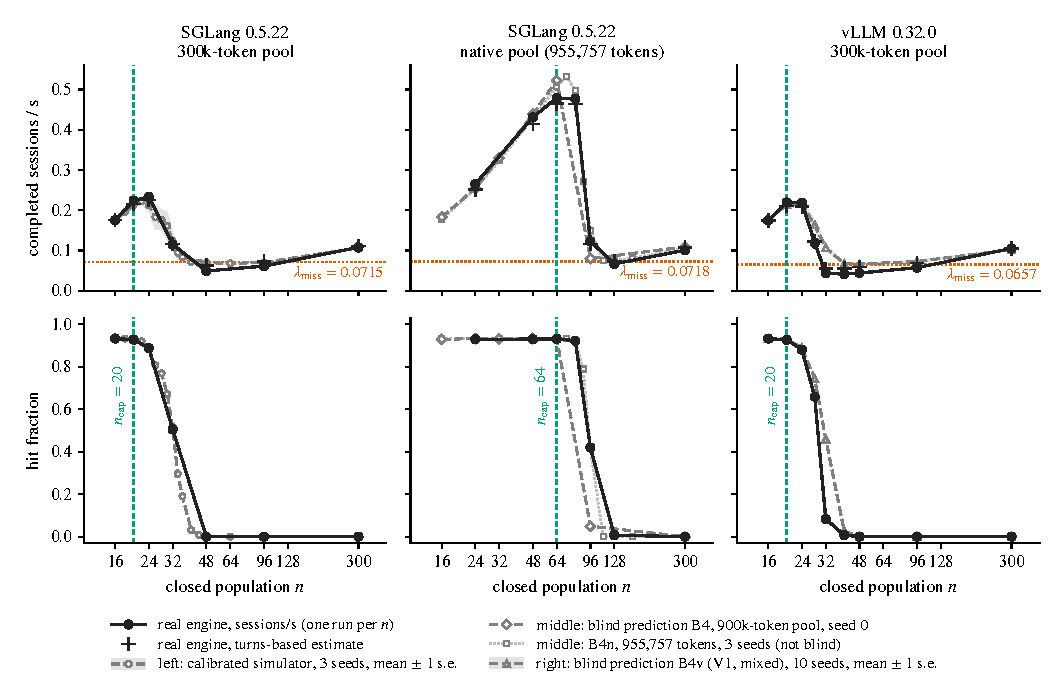
\includegraphics[width=0.92\textwidth]{figs/fig2_thrashing_curve.pdf}
\caption{Closed-population thrashing curve, real engine (black, filled; one run per $n$) against the simulator (gray, open, dashed). Top: $\mu(n)$ in completed sessions/s (plus signs: turns-based estimate); bottom: hit fraction. Left: SGLang, 300k-token pool; calibrated simulator, mean of 3 seeds $\pm$1 s.e. Middle: SGLang, native pool (955,757 tokens); blind prediction B4 at 900k tokens (seed 0); light gray, dotted: B4n at the real pool (3-seed mean), which is not blind (\S\ref{sec:blind}). Right: vLLM 0.32.0, 300k-token pool; blind prediction B4v (variant V1: token costs scaled to vLLM's all-miss rate; mixed batching), mean of 10 seeds $\pm$1 s.e. (\S\ref{sec:vllm}). Dotted: each cell's $\lmiss$. Green dashed: the registered caps, $n=20$, 64 and 20.}\label{fig:curve}
\end{figure*}

With the 300k pool (Fig.~\ref{fig:curve}, left), $\mu(n)$ rises from 0.176\sps{} at $n=16$ to 0.224 at 20 and 0.233 at 24, with hit fractions 0.93, 0.93 and 0.89. The run at $n=24$, which sets $\mu^*$, contains a degraded episode inside its window (hit fraction 0.66 over $[900,1200)$\,s, 0.46 in its worst 100\,s); over $[1200,2700)$\,s alone $\mu(24)=0.257$ against $\mu(20)=0.231$, so the near-tie that sets the cap of 20 owes part of its closeness to this episode. The run at $n=32$ mixes two regimes: degraded from about 450 to 2400\,s, then recovered to 0.80, for a hit fraction of 0.51. At $n=48$ none of the 20.0M prompt tokens in the window was served from cache: evictable tokens survive about 6.3\,s before eviction (estimated as mean evictable KV over the eviction rate) while a session returns after 30.6\,s on average (2.9\,s against 66\,s at $n=96$). The cliff is where memory predicts ($\Nlb\approx28.5$; the hit fraction crosses 0.5 at $n=32.2$), just below the all-miss onset $n_b=32.7$ of the first-principles model, which predicts this curve without using its points (\S\ref{sec:fp}, Table~\ref{tab:fpval}). Token-level hit rates have been reported to collapse as concurrent agents grow on SGLang~\citep{chen2026concur} and on vLLM~\citep{yuan2026agentic,hong2026misat}; what we add is $\mu(n)$ in completed sessions per second, the quantity the open-system model uses, at two pool sizes and, in \S\ref{sec:vllm}, on a second engine. Beyond the peak the curve is not monotone: it falls to $\mu(48)=0.049$\sps{} and rises again, $\mu(96)=0.061<\mu(300)=0.108$\sps. We attribute both to the synchronized start, which leaves old, long turns in the window at $n=48$ (served prompts 14\% above the stationary mean) and young sessions with short prompts at $n=300$ (71\% of the stationary length in flight); no longer run has tested this; the all-miss level implied by token throughput is roughly flat at 0.072--0.081\sps, so the collapse from the peak is about threefold. Stock LPM keeps 39\% of turns hitting at $n=48$ (rising from 0.28 to 0.44 through the window); at $n=300$ its queue of 269 exceeds the 128-request threshold above which, by the source, SGLang's LPM stops re-sorting its queue, and no turn hits; whether the fallback causes the zero was not tested (at $n=300$ the pool may be oversubscribed under any ordering).

With the native pool (Fig.~\ref{fig:curve}, middle), SGLang sized the KV pool at 955,757 tokens, 3.19 times the 300k pool. $\mu$ peaks at 0.479\sps{} at $n=64$ (0.477 at 80) with 92--93\% of turns hitting, then falls to 0.123 at $n=96$ (hit fraction 0.42), 0.067 at 128 (0.007) and 0.101 at 300. The hit fraction crosses 0.5 between $n=80$ (0.92) and 96 (0.42), near 93 by linear interpolation, against just above 32 at 300k; the peak is at 64--80 against 20--24. With one run per $n$, the cliff moves out roughly threefold. The all-miss capacity is unchanged within its standard error: $0.0718\pm0.0037$\sps{} turns-based against $0.0715\pm0.0038$, and $11{,}282\pm51$ against $11{,}243\pm84$ all-miss tokens/s. The 300k-token pool limit did not create the cliff; it moved it. The ratio $\mu^*/\lref$ is 6.67 with the native pool and 3.26 at 300k.\footnote{These are the registered values: the peak in completed sessions over the turns-based $\lref$. Turns-based over turns-based gives 6.48 and 3.15.}

\subsection{The all-miss capacity and the from-empty edge}\label{sec:edge}
E0a gives $\lref=0.0715\pm0.0038$\sps{} turns-based (standard error over three seeds), our estimate of $\lmiss$, $0.0717\pm0.0076$ in completed sessions, and $11{,}243\pm84$ all-miss prefill tokens/s. The token rate varies by $\pm1.2\%$ across seeds and the session rate by $\pm17\%$: the engine is bound by prefill tokens, and the sessions completed in 1800\,s are a small sample of a heavy-tailed quantity. The token rate divided by $E[W]$ gives 0.0728\sps, within 2\% of the turns-based value.

\begin{figure}[t]
\centering
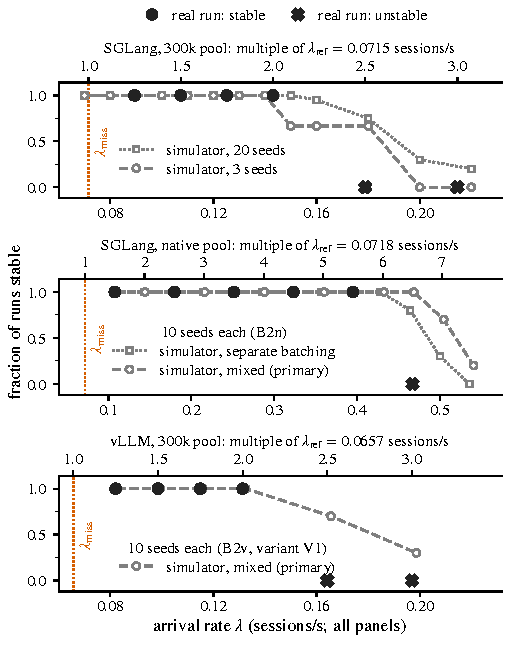
\includegraphics[width=\columnwidth]{figs/fig3_from_empty_stability.pdf}
\caption{From-empty stability. Real engine: one 3000\,s run per rate from an empty cache and queue (1 = stable, 0 = unstable), plotted at its nominal rate; all runs used arrival seed 0, whose realized rates were 6--13\% higher. Gray: blind simulator predictions, the fraction of simulated runs stable at multiples of the simulator's own $\lmiss$. Top, SGLang with the 300k pool: B2 (3 seeds dashed, 20 dotted). Middle, SGLang with the native pool: B2n (10 seeds; mixed batching, the primary mode, dashed; separate, dotted). Bottom, vLLM 0.32.0 with the 300k pool: B2v (variant V1, costs scaled to vLLM; mixed batching, 10 seeds). Top axes: multiples of each cell's $\lref$ (the simulators' own $\lmiss$ are 0.0722 at 300k, 0.0720 and 0.0714 native, and 0.0662 for B2v).}\label{fig:edge}
\end{figure}

From an empty cache and queue (Fig.~\ref{fig:edge}, top) the engine stayed stable at 1.25, 1.5, 1.75 and 2.0 $\lref$, ending each run with an empty queue and with 91--93\% of turns hitting over the run, and was unstable at 2.5 $\lref$ (final queue 127, rising by 146 over the last 1500\,s) and 3.0 (289 and 196). The edge lies between 2.0 and 2.5 $\lref$, well below $\mu^*/\lref=3.26$, so the from-empty edge, not the peak, bounds the window. The registered window was $(1,\,2.0)\,\lref=(0.0715,\,0.143)$\sps. Each rate is one 3000\,s run; a longer horizon could find a lower edge, and at 2.0 $\lref$ the hit fraction fell from 0.934 in $[300,1500)$\,s to 0.903 in the second half of the run. All six runs used seed 0, so they share one random-number stream: their arrival sequences are nested, and each arrival count lies about 2.1 standard deviations above its Poisson mean, 8--13\% above the nominal rate (302, 359, 416, 472, 585 and 697 sessions; the runs labelled 2.0 and 2.5 $\lref$ received 2.20 and 2.73 $\lref$). This makes the stable side of the bracket conservative and its unstable side weaker than the labels suggest; in realized arrivals the bracket is still below $\mu^*/\lref$.

With the native pool (Fig.~\ref{fig:edge}, middle; native E0b, rates in multiples of the native $\lref=0.0718$\sps) the engine stayed stable at 1.5, 2.5, 3.5, 4.5 and 5.5 $\lref$, ending each run with an empty queue and with 93\% of turns hitting over the run, and was unstable at 6.5 $\lref$: its final queue was 505, rising by 477 over the last 1500\,s, and its hit fraction fell from 0.84 in $[300,1500)$\,s to 0.00 in the second half. In nominal rates the edge lies between 5.5 and 6.5 $\lref$ (0.395 and 0.467\sps), so the native window is $(1,\,5.5)\,\lref$. Unlike at 300k, this does not show the edge below the peak ($\mu^*/\lref=6.67$, or 6.48 turns-based): these runs also used seed 0 (361 to 1478 sessions, 5.6--11.7\% above nominal), and the 6.5 run received 0.493\sps{} (6.86 $\lref$), above the measured peak, so overload alone can explain its instability. The stable 5.5 run received 0.419\sps{} (5.84 $\lref$). Its upper edge is 2.75 times higher than at 300k in units of $\lref$ (5.5 against 2.0), and the window is $4.5\,\lref$ wide against $1.0$. Again each rate is a single 3000\,s run.

\subsection{The registered paired test}\label{sec:e2}

\begin{table}[t]
\centering\footnotesize
\caption{The three registered tests: the two pre-registered SGLang tests, E2 (300k-token pool, cap 20, $\lref=0.0715$\sps) and native E2 (955,757-token pool, cap 64, $\lref=0.0718$\sps), and the registered vLLM test (300k-token pool, cap 20, $\lref=0.0657$\sps). States for seeds 0, 1, 2: T trapped, I indeterminate, D draining, G good, R recovered. Hit fraction, uncached prefill rate in multiples of the all-miss rate, mean backlog (sessions in the system) and its slope (sessions/s) over the evaluation window; ranges over seeds; good-arm slopes in absolute value. Slope thresholds: 0.0125, 0.0232, 0.0538 and 0.1077 at 1.35, 1.65, 2.5 and 4.0 $\lref$ on SGLang, 0.0115 and 0.0213 at 1.35 and 1.65 $\lref$ on vLLM. Rates are nominal; the base arrivals realized in the window, which the three arms of a seed share, were 1.45, 1.27, 1.42; 1.73, 1.61, 1.75; 2.73, 2.48, 2.58; 4.28, 3.89, 4.09; and on vLLM 1.45, 1.24, 1.41 and 1.76, 1.56, 1.74 $\lref$ for seeds 0, 1, 2.}\label{tab:e2}
\setlength{\tabcolsep}{3pt}
\resizebox{\columnwidth}{!}{%
\begin{tabular}{@{}c l c c c c c@{}}
\toprule
$\lambda/\lref$ & arm & states & hit & tokens & backlog & slope\\
\midrule
\multicolumn{7}{@{}l}{\emph{300k-token pool (E2)}}\\
1.35 & BURST   & T I T & 0.000 & 1.009--1.025 & 200--232 & 0.0036--0.0222\\
     & NOBURST & G G G & 0.930--0.934 & 0.08--0.09 & 7.9--9.7 & ${<}0.001$\\
     & CAPPED  & R R R & 0.930--0.934 & 0.08--0.09 & 7.9--9.7 & ${<}0.001$\\
\addlinespace
1.65 & BURST   & T T T & 0.000 & 1.025--1.029 & 283--332 & 0.0277--0.0362\\
     & NOBURST & G G G & 0.921--0.934 & 0.10--0.13 & 10.9--11.8 & ${<}0.002$\\
     & CAPPED  & R R R & 0.929--0.934 & 0.10--0.11 & 10.9--11.7 & ${<}0.002$\\
\midrule
\multicolumn{7}{@{}l}{\emph{native pool (native E2)}}\\
2.5  & BURST   & T T T & 0.000 & 1.074--1.078 & 557--601 & 0.079--0.085\\
     & NOBURST & G G G & 0.929--0.935 & 0.15--0.16 & 15.6--18.5 & ${<}0.003$\\
     & CAPPED  & R R R & 0.929--0.935 & 0.15--0.16 & 15.6--18.5 & ${<}0.003$\\
\addlinespace
4.0  & BURST   & T T T & 0.000 & 1.106--1.124 & 1098--1139 & 0.146--0.164\\
     & NOBURST & G G G & 0.929--0.935 & 0.24--0.27 & 28.2--33.6 & ${<}0.004$\\
     & CAPPED  & R R R & 0.929--0.935 & 0.24--0.27 & 28.1--33.5 & ${<}0.004$\\
\midrule
\multicolumn{7}{@{}l}{\emph{vLLM 0.32.0, 300k-token pool (registered, not pre-registered)}}\\
1.35 & BURST   & T D T & 0.000 & 0.995--1.012 & 201--222 & $-5\times10^{-5}$--0.0170\\
     & NOBURST & G G G & 0.930--0.931 & 0.07--0.09 & 7.0--8.4 & ${<}0.001$\\
     & CAPPED  & R R R & 0.930--0.931 & 0.07--0.09 & 7.0--8.4 & ${<}0.001$\\
\addlinespace
1.65 & BURST   & T I T & 0.000 & 0.948--1.018 & 281--330 & 0.0183--0.0341\\
     & NOBURST & G G G & 0.932--0.933 & 0.10--0.11 & 9.3--10.8 & ${<}0.001$\\
     & CAPPED  & R R R & 0.932--0.933 & 0.10--0.11 & 9.3--10.9 & ${<}0.001$\\
\bottomrule
\end{tabular}}
\end{table}

The registered analysis, run on all 18 runs with the code frozen at the registration commit, passes at both rates (Table~\ref{tab:e2}, top); by the definition of \S\ref{sec:prereg} the test is pre-registered. Every BURST run had a hit fraction of 0.000 over the evaluation window, an uncached prefill rate of 1.009--1.029 times the all-miss rate and a mean backlog of 200--332 sessions. One (1.35 $\lref$, seed 1) is stuck in the same way, but its backlog was flat over the window (207 sessions at its start, 206 at its end; slope 0.0036\sps, below the 0.0125 threshold), so the rule calls it indeterminate: its seed delivered 0.0910 arrivals/s in the window, 5.8\% below the nominal 0.0966 (seeds 0 and 2: 0.1037 and 0.1017), and the trapped engine completed 0.0913\sps. The pass at 1.35 $\lref$ therefore rests on 2 of 3 seeds, the minimum the rule allows. The other runs' base arrivals over the window came to 1.42 and 1.45 $\lref$ at 1.35 and 1.61--1.75 $\lref$ at 1.65 (Table~\ref{tab:e2}). Every NOBURST and CAPPED run is good (hit fractions 0.921--0.934, backlogs of 8--12 sessions, most asleep in tool calls); in the window CAPPED cannot be told apart from NOBURST, because the gate had drained the burst. The counts are small, and pooling the two rates does not make them independent: both rates use the same three seeds, with the same burst and nested arrivals (\S\ref{sec:harness}). BURST's hit fraction is below NOBURST's in all six seed-and-rate pairs; counting each seed once, a post-hoc one-sided sign test gives $p=1/8$, the smallest value three seeds allow.

In Fig.~\ref{fig:e2}, every BURST run is at zero hits from the window starting at 1300\,s to the end. Its backlog first fell, to 135--172 sessions 300--1300\,s after the burst, as short burst sessions finished, then rose; over the last 300\,s it was 206--369 sessions, still growing in five runs and flat in the sixth. The five trapped runs still completed 0.081--0.097\sps{} (1.13--1.35 $\lref$), above $\lmiss$, because the backlog's sessions are young and their turns short, so that at about the all-miss token rate more turns, and more sessions, complete (\S\ref{sec:fluid}), but below the arrival rate, and the sixth completed sessions about as fast as they arrived (1.28 and 1.27 $\lref$); only the uncached prefill rate sits at the all-miss level, which is why the registered rule uses tokens. The CAPPED gate's queue emptied 1547--1904\,s after the burst at 1.35 $\lref$ and 2021--2693\,s at 1.65 $\lref$, 3--52\% longer than the fluid estimate of \S\ref{sec:props} from the population present at the burst (1453--1508\,s and 1757--1804\,s; the registration's cruder estimate was 1571\,s and 1889\,s), and well before the evaluation window. Outside the registered criteria, the CAPPED arm's hit fraction dips while the gate drains the burst: its lowest 100\,s window is 0.48--0.77 in four of six runs, against 0.82--0.89 for NOBURST, which plausibly slowed the drain. The cap has a cost that the registered criteria do not measure: it turns the burst into admission delay at the client. In each CAPPED run 349--543 sessions waited at the gate, 45--66\% of them ordinary arrivals queued behind the burst, for 405--471\,s on average and at most 853--985\,s; outside the drain the gate bound only briefly, when arrivals clustered (at most 40 sessions in a run, each for less than 50\,s). Without the cap, turns completed in the BURST arm's evaluation window took a mean of 163--237\,s from send to completion (the client does not stream), against 1.4--1.7\,s in NOBURST and CAPPED and 1.4--1.5\,s in every arm before the burst; at 8700\,s, 19--29\% of BURST sessions were unfinished. So at loads that the engine carried from empty for the full 8700\,s run (E0b carried the bracketing rates, 1.25--1.75 $\lref$, for 3000\,s), 200 sessions arriving within a minute, an order of magnitude more than the 8--12 present in the good state, moved it into an all-miss state that it did not leave within 7500\,s, and a cap of 20 sessions, within 5\% of the measured peak of $\mu(n)$ (argmax $n=24$), prevented that at the price of that admission delay. The heuristic F2 of \S\ref{sec:fp} puts the probability that a run at these rates leaves the good state on its own within 8700\,s at about 0.5\% at 1.35 and 5\% at 1.65 $\lref$, so good NOBURST arms over 8700\,s are the expected outcome, not evidence that the good state never ends.

\subsection{The registered test with the native pool}\label{sec:e2native}

\begin{figure*}[t]
\centering
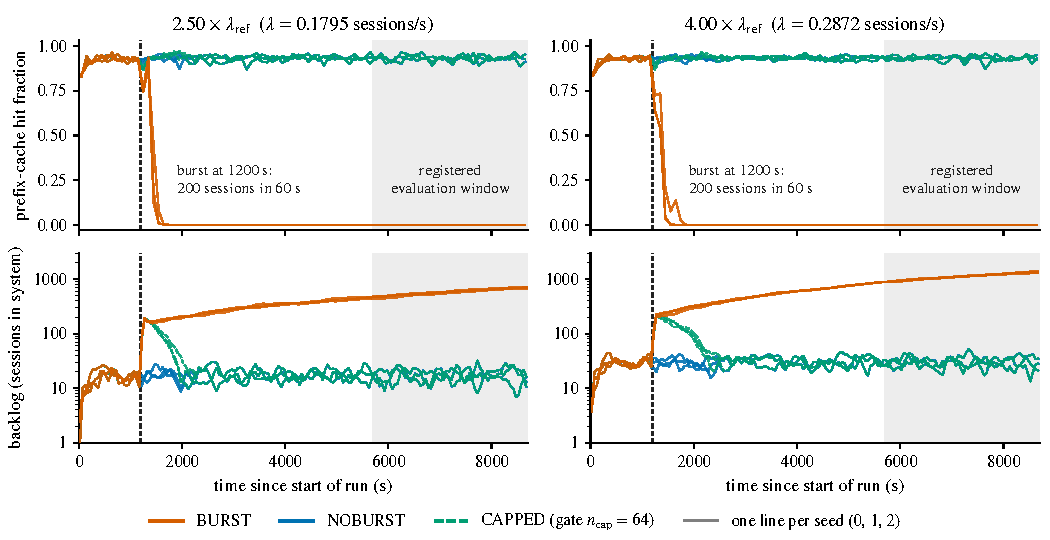
\includegraphics[width=\textwidth]{figs/fig7_e2_native_timeseries.pdf}
\caption{The registered test with the native pool (native E2) at 2.5 $\lref$ (left) and 4.0 $\lref$ (right), $\lref=0.0718$\sps; layout as in Fig.~\ref{fig:e2}, with the CAPPED gate at $\ncap=64$ and the backlog axis extended to 3000.}\label{fig:e2native}
\end{figure*}

A second registration was filled by the same formulas from the native curve, the native E0a calibration and the native E0b bracket, and committed before the first native E2 job (Appendix~\ref{app:prereg}). Its window is $(1,\,5.5)\,\lref$; the one-third/two-thirds rule, written down before native E0b was read, gives 2.5 and 4.0 $\lref$ (0.1795 and 0.2872\sps); the cap rule gives $\ncap=64$, the peak (flagged ambiguous: $\mu(80)$ is within 0.35\% of $\mu(64)$). The protocol, the burst of 200 sessions and the trap rule are E2's, with the native reference rates.

The registered analysis passes at both rates, and every run is in the predicted state (Table~\ref{tab:e2}, bottom; Fig.~\ref{fig:e2native}); by the definition of \S\ref{sec:prereg} this test, too, is pre-registered. All six BURST runs were trapped: hit fraction 0.000 over the evaluation window, an uncached prefill rate of 1.074--1.078 (2.5 $\lref$) and 1.106--1.124 (4.0 $\lref$) times the native all-miss rate of 11,282 tokens/s, and mean backlogs of 557--601 and 1098--1139 sessions with slopes above the threshold. All six NOBURST runs were good and all six CAPPED runs recovered (hit fractions 0.929--0.935, backlogs of 16--34 sessions, most asleep in tool calls). Over the window the base arrivals were 2.48--2.73 $\lref$ at 2.5 and 3.89--4.28 at 4.0. Counting each seed once, the post-hoc sign test again gives $p=1/8$. Pooled post hoc over the two pre-registered SGLang tests (a descriptive count, not a registered quantity: the tests differ in pool, cap and rates, and reuse the same three seeds, so the 12 runs of each arm share three seeds' session sequences), NOBURST was good and CAPPED recovered in 12 of 12 runs each, and BURST was at zero hits in 12 of 12 and trapped by the rule in 11 of 12.

With the larger pool the collapse took longer and the backlog never drained (Fig.~\ref{fig:e2native}). In the 100\,s window that contains the burst, the native BURST runs still hit with 0.99--1.00 of their follow-up turns (all but 4 of 3,326), against 0.43--0.59 at 300k; counting the burst's own first turns, which always miss, they hit with 0.63--0.76 of all turns (0.21--0.33 at 300k). Every BURST run was at zero hits from 300--600\,s after the burst to the end of the run. In 50\,s bins its backlog fell after the burst only at 2.5 $\lref$, to 155--168 sessions 150--200\,s after it; at 4.0 $\lref$ it grew from the first bin after the burst (201--231 sessions). It then grew to 658--1379 sessions over the last 300\,s. The trapped engine completed 0.103--0.146\sps{} (1.44--2.03 $\lref$), above $\lmiss$, because its backlog's sessions are young and their turns short (\S\ref{sec:fluid}), and well below the arrival rates; it prefilled 1.074--1.124 times the 32-session all-miss token rate, as the simulator predicted (\S\ref{sec:blind}). The CAPPED gate's queue emptied 512--583\,s after the burst at 2.5 $\lref$ and 837--937\,s at 4.0, between 4\% shorter and 13\% longer than the fluid estimate from the population present at the burst (491--518\,s and 840--876\,s), and 10--23\% shorter than the registration's cruder 668\,s and 1043\,s. Here 234--448 sessions waited at the gate, 128--180\,s on average and at most 247--361\,s; outside the drain the gate bound for at most 6 sessions in a run, each for at most 7.1\,s. BURST turns completed in the evaluation window took 321--511\,s on average, against 1.6--2.5\,s in NOBURST and CAPPED, and 38--50\% of BURST sessions were unfinished at 8700\,s. Here 200 sessions were 6 to 13 times the 16--34 present in the good state. B3n had predicted a pass at somewhat higher rates (\S\ref{sec:blind}).

\subsection{A second engine: vLLM}\label{sec:vllm}
vLLM 0.32.0 passed its smoke test on the same GPU type (token ids and cached-token counts returned, flush verified) and ran with the SGLang cell's settings where they exist: FCFS, prefix caching on, chunked prefill of 8192 tokens, at most 256 running requests and a 300,000-token pool (18,750 blocks of 16 tokens). With prefix caching off, its all-miss capacity (vLLM E0a, three seeds) is $0.0657\pm0.0030$\sps{} turns-based and $10{,}349\pm81$ uncached prefill tokens/s, 8\% below SGLang's 0.0715 and 11,243 on the same model, GPU and workload.

Six exploratory BURST runs came first, under a registration derived from E2's: the multiples 1.35 and 1.65 of vLLM's own $\lref$ (0.0886 and 0.1083\sps), seeds 0, 1, 2, and E2's protocol and trap rule with vLLM's reference rates. Their window and multiples were inherited from the SGLang cell, not measured: these runs preceded vLLM's own closed curve and from-empty edge, and no NOBURST or CAPPED arm ran with them. Before the burst all six runs were in the good state (hit fraction 0.93--0.94 from 300\,s to the burst; a post-hoc reading). After it, all six were at zero hits from the 100\,s window starting 100\,s after the burst to the end of the run (also a post-hoc reading), with an uncached prefill rate of 0.997--1.031 times vLLM's all-miss rate and mean backlogs of 203--227 sessions at 1.35 and 277--309 at 1.65 $\lref$ (Fig.~\ref{fig:grid}, bottom row). The registered rule calls four of them trapped. The other two are indeterminate by the slope test: one has a flat backlog near 203 sessions (slope 0.0002 against a threshold of 0.0115; 1.35 $\lref$, seed 1), and in the other the backlog grew from 269 to 294 sessions over the window, at 0.0175 against 0.0213 (1.65 $\lref$, seed 1). Both are seed 1, as are the indeterminate SGLang FCFS runs at 1.35 $\lref$ with and without the refresh. A vLLM run's arrivals are a subset of the SGLang run's at the same seed and multiple, and seed 1 delivered 5.5--7.9\% fewer arrivals than nominal in these windows, so the labels on the two engines agree on the same workloads rather than on independent ones. So the same all-miss state appears on a second engine after the same burst. Without control arms these runs are not a registered paired test: they do not show that vLLM's good state would have lasted the run without the burst, or that a cap would have recovered it.

vLLM's own closed curve (Fig.~\ref{fig:curve}, right; one run per $n$) has the shape of SGLang's at the same pool. $\mu(n)$ peaks at 0.219\sps{} at $n=20$, with $\mu(24)$ 0.5\% lower, so the peak is a tie at one run per $n$; $\mu^*/\lref=3.34$ (3.21 turns-based). The hit fraction is 0.93 at $n\le20$, 0.88 at 24, 0.66 at 28, 0.08 at 32 and 0.0075 at 40; it crosses 0.5 near $n=29.1$, close to $\Nlb$, and $\mu$ falls 80\% from $n=24$ to 32. The closed curve had no cache hits from $n=48$ on, as with SGLang's FCFS; Proposition~\ref{prop:A}, a limit statement, is consistent with this but does not predict it. Like SGLang's, the curve is not monotone beyond its peak: in completed sessions it falls to 0.63--0.67 $\lref$ at $n=32$--48 (0.83--0.90 turns-based), whose windows held old, long turns (served prompts 12--17\% above the stationary mean), and rises to 1.60 $\lref$ at $n=300$ (1.59 turns-based). vLLM preempted running requests in every closed run from $n=24$ on (12 to 72 per run from $n=32$ on), which the proposition allows on our reading of vLLM's source (Appendix~\ref{app:proofs}).

From an empty cache and queue (Fig.~\ref{fig:edge}, bottom; one 3000\,s run per rate) vLLM stayed stable at 1.25, 1.5, 1.75 and 2.0 $\lref$ (0.082--0.131\sps), ending each run with an empty queue and with 92--93\% of turns hitting, and was unstable at 2.5 $\lref$ (final queue 82, rising by 94 over the last 1500\,s) and 3.0 (247 and 175). The edge lies between 2.0 and 2.5 $\lref$, as on SGLang with the same pool, so vLLM's window is $(1,\,2.0)\,\lref$. These runs also used seed 0 and received 8.6--13.3\% more arrivals than nominal (279 to 642 sessions; the runs labelled 2.0 and 2.5 $\lref$ received 2.21 and 2.74 $\lref$), but the unstable 2.5 run's realized 0.180\sps{} is below the measured peak (0.219, or 0.211 turns-based), so here, as at 300k on SGLang and unlike with the native pool, the edge lies below the peak.

Blind predictions for this cell, B4v for the curve and B2v for the edge, were made with the calibrated simulator in two variants, unchanged and (V1) with its token costs scaled so that its all-miss token rate matches vLLM's measured one (a fit to vLLM's E0a, not a prediction), each in both batching modes, and are frozen in \fpath{notes/PREDICTIONS_vllm.md}. They were committed and pushed to GitHub before any of the curve and edge runs had finished, but 22 minutes after the jobs were submitted, when two of them had been running for almost as long; they are blind in that no result existed, not in submission order. The peak level and the cap held: B4v (V1, mixed batching, 10 seeds) put the peak at $n=24$ with 0.215\sps{} turns-based, against the real 0.211 at $n=20$ (0.210 at 24), and the cap at 20. The real cliff is steeper and earlier than predicted: hit fractions of 0.66 against 0.74 at $n=28$ and 0.08 against 0.46 at $n=32$ (0.46--0.53 over the four simulator configurations), and a 0.5 crossing near 29.1 against 31.4--32.6. B2v put the edge at 2.0 $\lref$ in all four configurations (V1 with mixed batching: 10 of 10 runs stable through 2.0, 7 of 10 at 2.5 and 3 of 10 at 3.0), as measured. The simulator does not model vLLM's block-level eviction or its scheduler and token budget; like vLLM, and unlike SGLang, it has no waiting-prefix refresh.

A registration for vLLM was then filled by the formulas used for SGLang (Appendix~\ref{app:prereg}) from this curve, vLLM's E0a and five of the six E0b runs (the 3.0 $\lref$ run was still running; it came out unstable, which leaves the bracket unchanged). It gives the window $(1,\,2.0)\,\lref$ with $\lref=0.06566$\sps, the points 1.35 and 1.65 $\lref$ by the one-third/two-thirds rule, which was written in our status notes before any vLLM curve or edge existed, and $\ncap=20$, flagged ambiguous because $\mu(24)$ lies within 0.5\% of the peak. The protocol, the burst and the trap rule are E2's. The points equal the multiples of the exploratory runs; the rule that selected them was adopted for vLLM (\texttt{836063a}) after their outcome was known, and the BURST arm reuses their seeds 0--2 and so their arrivals: it is not an independent replication of them. The registration was committed 37\,s before the 18 jobs of the paired test were submitted, but reached GitHub 2\,min after the submission and 53\,s after the first job had started, before any job had finished; by our definition (\S\ref{sec:prereg}) this test is therefore registered but not pre-registered. At 18:21 CDT the memory request of the 15 jobs still pending (17166124--38) was lowered from 128G to 48G so that they could be scheduled; no code, argument or registration changed, and no job had ended. The third prediction round, frozen before the registration existed, also predicted this test (B3v): a pass at both points in all four simulator configurations, with every simulated BURST run at zero hits (7 to 9 of 10 per point trapped by the rule, the rest indeterminate), NOBURST good in 10 of 10 and CAPPED at a cap of 20 recovered in 10 of 10. Because the session that specified that round knew the exploratory BURST outcomes, the BURST-arm part of B3v is blind at most on the predicting agent's side, and there only by instruction and by the agent's own unchecked record: its copy of the repository held those runs (Appendix~\ref{app:timeline}).

The registered analysis passes at both rates (Table~\ref{tab:e2}, bottom): at each rate, in two of three seeds BURST was trapped, NOBURST good and CAPPED recovered. Its tool also labels the test pre-registered and decisive, labels it assigns by commit order (as it did for the two SGLang tests); by the definition of \S\ref{sec:prereg} this test is registered, not pre-registered. Every BURST run had zero hits over the evaluation window and prefilled 0.948--1.018 times vLLM's all-miss token rate. The two runs the rule does not call trapped are both seed 1, the seed with the fewest arrivals in the window (1.24 and 1.56 $\lref$ at the nominal 1.35 and 1.65). At 1.35 its backlog stayed flat at about 200 sessions with an uncached prefill rate of 1.007 times the all-miss rate, and the rule labels it draining because its fitted slope was $-5\times10^{-5}$\sps: it was stuck, not draining. At 1.65 it was indeterminate by the slope test (0.0183 against 0.0213). The pattern repeats the exploratory runs, whose arrivals these BURST runs share. Over the last 300\,s the BURST backlog was 196--250 sessions at 1.35 and 299--383 at 1.65 $\lref$; turns completed in the window took 180--261\,s on average, against 1.4--1.6\,s in the other arms, and 20--31\% of BURST sessions were unfinished at 8700\,s. NOBURST stayed good and CAPPED recovered in all six runs each (hit fractions 0.930--0.933). In each CAPPED run 322--499 sessions waited at the gate, 43--63\% of them ordinary arrivals, for 413--526\,s on average and at most 1053\,s, and the gate's queue first emptied 1521--2735\,s after the burst, 1.05--1.63 times the fluid estimate from the population present at the burst. B3v had predicted a pass at both rates; the trapped runs' token rates lay at or below its range (0.948--1.018 against 0.99--1.07). The first-principles model, pushed at 02:05:30 CDT, three minutes before the registered verdict was computed and, by the vLLM session's record (\fpath{notes/LOG.md}), before any of these run directories was opened, predicted good-state hit fractions of 0.932 and gate drains of 1449 and 1725\,s, short of the measured 1521--2027 and 1848--2735\,s, as in three of the four SGLang cells (Table~\ref{tab:fpval}); the theory's own blindness declaration does not cover these runs. Across the three registered tests, BURST was at zero hits in 18 of 18 runs and trapped by the rule in 15, NOBURST was good in 18 of 18 and CAPPED recovered in 18 of 18; the tests share seeds, and vLLM's BURST arm shares arrivals with earlier runs, so these counts are descriptive.

Mechanism predictions for this test were frozen and pushed at 18:20:13 CDT on 2026-10-30, before any of its 18 runs had ended (\fpath{configs/r11_mechanism_predict.yaml} and \fpath{notes/PREDICTIONS_r11_mechanism.md}, commit \texttt{f1338e3}; byte copies under \fpath{r11_mechanism/frozen/} in the test's data directory). They were: (a) in NOBURST and CAPPED, a median gap between a session's turns below 0.05 times the pool's turnover time $R_M=M/\text{churn}$ (\S\ref{sec:mechanism}) and a follow-up hit fraction above 0.95, and in BURST a ratio above 2 and a hit fraction below 0.05; (b) in BURST, a mean KV usage of at least 0.90 and an uncached prompt-token rate within 15\% of the all-miss rate, that is, a full pool rewritten at the all-miss rate; (c) an online detector, a follow-up hit fraction below 0.2 over 60\,s, alarming within 300\,s of the burst in every BURST run and never after 600\,s in a good arm; (d) an engine rule, a mean time to first token above 30\,s over 100\,s, behaving the same way. The frozen decision rule required (b) and (c) in every BURST run and (a) and (c) in all good-arm runs but at most one. (a), (b) and (d) held in all 18 runs: the gap ratio was 6.44--8.78 in BURST and 0.014--0.022 elsewhere; in BURST the KV usage was 0.920--0.937 and the uncached rate 0.871--0.955 times the all-miss rate; and the engine rule alarmed 170--210\,s after the burst in BURST and never in a good arm. (c) failed. The detector alarmed 100--120\,s after the burst in every BURST run, but also in two CAPPED runs, seed 2 at both rates, 880 and 820\,s after the burst, while the gate was draining with 20 sessions admitted and 123--143 waiting; the follow-up hit fraction dipped to 0.06--0.17 for 20--40\,s and was above 0.8 again 110--160\,s later. The frozen decision rule is therefore not met. The detector uses CONCUR's hit-rate threshold (0.2) without its KV-usage condition~\citep{chen2026concur}; we do not claim it, and a deployed alarm on this rule would have fired twice without a trap. The bands of (a)--(d) were chosen on the SGLang runs and on the exploratory vLLM runs, whose arrivals the BURST arm repeats, so only the NOBURST and CAPPED checks are out of sample.

\subsection{The sustaining variable}\label{sec:mechanism}
At the same arrival rate the good and the trapped state differ in how long a session's KV lies idle between turns compared with how long the pool keeps idle KV. Let the gap of a follow-up turn be the time from the completion of its session's previous turn to its own completion, the tool time plus the turn's latency, and let $R_M=M/\text{churn}$, where churn is the rate at which new KV is written (uncached prompt tokens plus completion tokens per second). Under LRU an idle prefix is evicted by the time $M$ newer tokens have been written, so a follow-up whose idle time, from its session's previous completion to its own admission, exceeds $R_M$ misses. This is Denning's criterion, an interval between references longer than the window~\citep{denning1968working}, with Che's characteristic time as the window~\citep{che2002hierarchical}, and it has been stated for LLM prefix caches whose revisit times are set by routing~\citep{cheng2026cacheroute}. The gap, the statistic frozen for the vLLM mechanism checks, exceeds the idle time by the turn's own service, and on SGLang the LRU refresh of the first 128 waiting requests' prefixes (\S\ref{sec:background}) resets the age of some waiting prefixes, so gap$/R_M$ is a proxy for the criterion, not the criterion itself. Table~\ref{tab:gapR} gives the median gap over $R_M$ in every arm of the three registered tests, computed by the script frozen for the vLLM mechanism checks (\S\ref{sec:vllm}). In every good-state run the ratio is 0.010--0.028: the gap is 4.9--5.9\,s, mostly tool time, and $R_M$ is 188--505\,s. In every BURST run it is 4.1--9.7: $R_M$ falls to 26--78\,s because the trapped engine rewrites the pool at the all-miss rate, and the gap rises to 166--516\,s, of which the mean tool time is 4.8--5.1\,s and the rest is the turn's latency. Turn latency, not tool time, carries the gap past $R_M$; a turn's own service takes seconds (its latency is 1.4--2.5\,s in the good state), so most of that latency is time in the queue. That queueing behind other agents lengthens the gap between an agent's turns has been measured for the host KV tier of a closed pool of agents, and its backlogged-pool working-set scale is the cycle argument behind the identity below, stated there as an approximation~\citep{shao2026efficientagent}; what we add is the measurement in both states at one load and the identity's exact time-domain form. The trapped value obeys a cost-model-free identity: when every present session completes one turn per cycle of the FCFS queue, gap$/R_M$ equals the total next-turn context of the sessions present divided by $M$ (Proposition~\ref{prop:trapid}), and the round-robin layer of the first-principles model (\S\ref{sec:fp-heur}), driven only by the arrival rate and the burst, gives values within 4\% of the measured means (Table~\ref{tab:gapR}). These are correlations across two states at one load; whether a temporary increase in tool latency, with no burst, can trigger the trap is the registered TOOLSLOW test of \S\ref{sec:frozen}, which would not separate the gap from the capacity loss that the slowdown also causes. The look-aside caches of the metastability literature fail to refill after losing their contents~\citep{bronson2021metastable,huang2022metastable,farahbakhsh2026characterizing}; here the pool is full and rewritten before reuse, which in Huang et al.'s terms is capacity-degradation amplification.

\begin{table}[t]
\centering\footnotesize
\caption{The sustaining variable: median gap between a session's turns over the pool's turnover time $R_M=M/\text{churn}$, over the evaluation window, ranges over seeds (good arms: NOBURST and CAPPED). Gap: median, seconds. Model: Proposition~\ref{prop:trapid} applied to the turn mix and backlog that the round-robin layer RR of the first-principles model predicts (\S\ref{sec:fp-heur}; tag \texttt{r13-theory-pred}; for vLLM validated on the exploratory runs, whose arrivals the registered BURST arm repeats). Computed by \fpath{analysis/r11/loopvars_frozen.py} (commit \texttt{f1338e3}), unchanged.}\label{tab:gapR}
\setlength{\tabcolsep}{2pt}
\begin{tabular}{@{}l c c c c c c@{}}
\toprule
 & & \multicolumn{2}{c}{good arms} & \multicolumn{3}{c}{BURST}\\
test & $\lambda/\lref$ & gap$/R_M$ & $R_M$ (s) & gap$/R_M$ & gap (s) & model\\
\midrule
SGLang 300k & 1.35 & 0.016--0.020 & 255--307 & 6.35--6.92 & 166--178 & 6.93\\
            & 1.65 & 0.022--0.028 & 188--230 & 8.18--9.67 & 210--249 & 8.98\\
SGLang native & 2.5 & 0.010--0.012 & 446--505 & 4.14--4.57 & 322--354 & 4.45\\
            & 4.0 & 0.018--0.022 & 272--310 & 6.68--6.96 & 504--516 & 7.06\\
vLLM 300k   & 1.35 & 0.014--0.017 & 286--337 & 6.44--6.79 & 183--196 & 6.64\\
            & 1.65 & 0.019--0.022 & 229--264 & 8.16--8.78 & 231--261 & 8.52\\
\bottomrule
\end{tabular}
\end{table}

\subsection{Blind predictions against outcomes}\label{sec:blind}

\begin{table}[!tp]
\centering\footnotesize
\caption{Blind predictions (calibrated simulator, mixed batching unless noted) against outcomes; rates in sessions/s; native and vLLM rates in multiples of $\lmiss$ (for the simulator its own, for the engine that cell's $\lref$). Percentages in the last column are predicted/real $-1$. B1 is not blind in time and is close to the calibration data (\S\ref{sec:sim}, Appendix~\ref{app:timeline}). B3 and B3n used a per-arm pass rule (each arm in 2 of 3, resp.\ 7 of 10, seeds); the registered rule asks for all three arms in the same seed, which B3n's runs also meet (9 of 10 seeds at its low mixed point, 10 of 10 elsewhere). B3's token-ratio and backlog ranges are over the two simulated rates that bracket each registered rate. B4 is the registered seed~0 on the grid $n=48$, 64, 96 (supplementary 5-seed means: peak 0.514, $\mu(96)=0.085$, $\mu(300)=0.108$). B2n and B3n: 10 seeds (``sep.'': separate batching); B3n's low and high points are 2.85 and 4.65 (sep.\ 2.65 and 4.35). B4v and B2v: vLLM, variant V1 (simulator token costs scaled to vLLM's all-miss rate), 10 seeds, turns-based rates. B3n is blind in time; B2n, B4v and B2v were pushed after their jobs were submitted, before any run had finished (\S\ref{sec:vllm}); B4n (3-seed mean) is not blind. B3v: vLLM paired test, all four configurations (V0, V1; mixed, separate), 10 seeds; blind in time, its BURST part blind only on the predicting agent's side (\S\ref{sec:vllm}).}\label{tab:blind}
\setlength{\tabcolsep}{2.5pt}
\begin{tabular}{@{}l l l@{}}
\toprule
 & predicted & real\\
\midrule
B1 & $\lmiss$ 0.0722 (turns) & 0.0715 ($+0.9\%$)\\
   & 11,220 tokens/s & 11,243 ($-0.2\%$)\\
   & $\lmiss$ 0.0694 (sessions) & 0.0717 ($-3.1\%$)\\
\addlinespace[1pt]
B2 & all-stable edge 0.14 (3 seeds), 0.15 (20) & in $[0.143,\,0.179)$\\
   & at 0.18: 2/3 stable (15/20) & 0.179 unstable\\
\addlinespace[1pt]
B3 & PASS at all rates 0.09--0.16 & PASS at 0.0966, 0.1180\\
   & \quad 20 seeds: sep.\ fails at 0.16 & \quad (0.16 not run)\\
   & token ratio 1.003--1.027 (0.09--0.10) & 1.009--1.025 (0.0966)\\
   & \quad 1.025--1.043 (0.11--0.12) & 1.025--1.029 (0.1180)\\
   & backlog 171--234 (0.09--0.10) & 194--226 requests\\
   & \quad 253--313 requests (0.11--0.12) & 277--325\\
   & good-arm hit 0.929--0.937 & 0.921--0.934\\
   & trapped 3/3 at 0.09 and 0.10; & trapped 2/3 at 0.0966\\
   & \quad 20 seeds: 14/20, 18/20 & \\
\addlinespace[1pt]
B4 & peak $n=64$, $\mu$ 0.523 (900k) & $n=64$, 0.479 ($+9\%$)\\
   & 0.5-hit crossing $\approx$80 & $\approx$93 ($\approx$91 on B4's grid)\\
   & $\mu(96)=0.079$, $\mu(300)=0.109$ & 0.123, 0.101\\
\midrule
B2n & all-stable edge 6.5; sep.\ 6.0 & in $[5.5,\,6.5)$\\
    & at 6.5: 10/10 stable; sep.\ 8/10 & 6.5 unstable\\
    & at 1.5--5.5: 10/10 stable, both & stable\\
\addlinespace[1pt]
B3n & PASS at 2.85, 4.65; sep.\ 2.65, 4.35 & PASS at 2.5, 4.0\\
    & trapped token ratio 1.086--1.109 (low) & 1.074--1.078 (2.5)\\
    & \quad 1.119--1.140 (high) & 1.106--1.124 (4.0)\\
    & trapped backlog 460--643 (low) & 549--594 requests\\
    & \quad 1067--1333 requests (high) & 1089--1130\\
    & good-arm hit 0.928--0.936 & 0.929--0.935\\
    & BURST trapped 9/10 to 10/10 & 3/3 at both\\
\addlinespace[1pt]
B4n & peak $n=72$, $\mu$ 0.532 & 64--80, 0.479 ($+11\%$)\\
    & 0.5-hit crossing 94; hit 0.42 at 96 & $\approx$93; 0.42\\
    & cap 64, 0.35\% inside the rule & 64\\
\midrule
B4v & peak $n=24$, $\mu$ 0.215; cap 20 & $n=20$, 0.211 ($+2\%$); 20\\
    & hit 0.74 at $n=28$, 0.46 at 32 & 0.66, 0.08\\
    & 0.5-hit crossing 31.4 & 29.1\\
\addlinespace[1pt]
B2v & all-stable edge 2.0; at 2.5: 7/10 & in $[2.0,\,2.5)$; 2.5 unstable\\
\addlinespace[1pt]
B3v & PASS at 1.35, 1.65 (all four) & PASS at both\\
    & BURST trapped 7--9/10 & 2/3 at each\\
    & NOBURST, CAPPED(20) 10/10 & 3/3 and 3/3 at each\\
    & trapped token ratio 0.99--1.07 & 0.948--1.018\\
\bottomrule
\end{tabular}
\end{table}

B1 matched within 3.1\% (Table~\ref{tab:blind}), which mostly checks the simulator's bookkeeping (\S\ref{sec:sim}). B2's edge, 0.14--0.15\sps, is consistent with the real edge in $[0.143,\,0.179)$; near 0.179 the model keeps 2 of 3 runs stable (15 of 20 with more seeds), so one unstable run there is no contradiction. B3 predicted a pass at every tested rate in both batching modes. At the simulated rates that bracket each registered rate, the primary (mixed) mode's trapped token ratios, 1.003--1.027 at 0.09--0.10\sps{} and 1.025--1.043 at 0.11--0.12, contain the observed 1.009--1.025 at 0.0966 and 1.025--1.029 at 0.1180; but at 0.12, the grid point nearest the higher rate, the prediction was 1.034--1.043, above what the engine did. The observed good-arm hit fractions (0.921--0.934) are close to, and at the low end partly below, the predicted 0.929--0.937. B3 flagged both ends of its grid as fragile. At the low end the slope margin $0.5(\lambda-\lmiss)$ is small: with its registered three seeds it trapped 3 of 3 at both 0.09 and 0.10, but with 20 seeds 14 and 18, so 10--30\% of runs there are stuck without meeting the slope test; one indeterminate real run in three at 0.0966 is consistent with that. At 0.16 the 20-seed supplement of the secondary (separate) mode failed the pass rule, with NOBURST good in 13 of 20 seeds, one short; the engine was not run there. (Backlogs compare only roughly: the simulator counts waiting requests, the engine runs outstanding ones.) B4 got the peak's position, within its coarse grid, and the outward shift of the cliff; the predicted peak was 9\% above the real one and the cliff early: on B4's grid of 64 and 96 the real hit fraction crosses 0.5 near 91, against B4's 80, and at $n=96$ the engine still hit 42\% of turns, against B4's 5\%. The early cliff is mostly the pool: B4n, the same simulator at the real pool (not blind), hit 0.42 at $n=96$ and crossed 0.5 near 94. The peak error is not: at $n=64$, where nothing is evicted, seed 0 gives the same 0.523 in both pools. Two qualifications: the verifier's strict check that every B3 pass lies inside the B2 all-stable range failed (B3 asks for 2 of 3 seeds over a longer run), and B2 is blind only by instruction (checked afterwards from the agents' transcripts) and by commit order, not by event order: E0b had finished on the cluster before the predictions were committed, and was pulled 13 minutes after their commit reached GitHub.

The second round, for the native pool, held in part: B3n's pass held at the registered rates, which lie 6--16\% below its own test points, with trapped token rates, backlogs and good-arm hit fractions consistent with the lower rates; the primary mode of B2n put the from-empty edge at least one grid step too high; and B1n and B4n are not blind (Appendix~\ref{app:supp}). For vLLM, B4v and B2v got the peak level, the cap and the edge right but predicted a later and gentler cliff, and B3v's pass held (\S\ref{sec:vllm}).

\subsection{Exploratory policy grid}\label{sec:grid}

\begin{figure}[t]
\centering
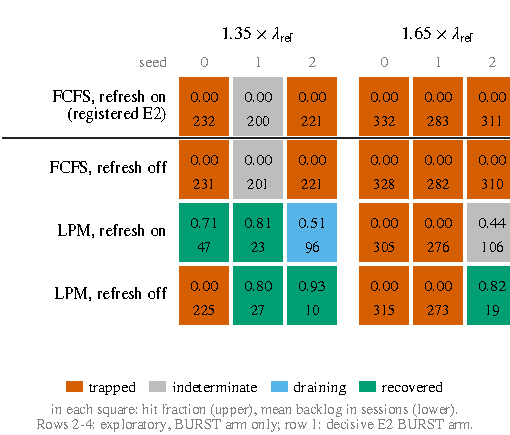
\includegraphics[width=\columnwidth]{figs/fig6_policy_grid.pdf}
\caption{Exploratory policy grid, BURST arm only, 300k pool. Rows: FCFS with the waiting-prefix refresh (the registered runs), FCFS without, LPM with, LPM without (under LPM the refresh acts only during the FCFS fallback above 128 waiting requests); below the dashed line, the exploratory vLLM 0.32.0 runs with FCFS (\S\ref{sec:vllm}), at multiples of its own $\lref$ (0.0657\sps). Columns: 1.35 and 1.65 $\lref$ by seed. Colour: registered state (RECOVERED judged on the last 300\,s); numbers: hit fraction and mean sessions in the system over the evaluation window.}\label{fig:grid}
\end{figure}

Three other engine cells ran the BURST arm at the registered rates and seeds (Fig.~\ref{fig:grid}) under exploratory registrations derived from E2's, with no control arms. In these runs the refresh made no difference for FCFS: all six runs without it, which share their arrivals with the registered runs, have the registered runs' states, hit fraction 0.000 and backlogs within 1.3\% of theirs (201--231 sessions at 1.35 $\lref$, 282--328 at 1.65), as the source predicts: the refresh moves waiting prefixes up the LRU order but does not pin them. Both rates lie inside the window; near $\lmiss$, with a cap or with the native pool, the refresh was not tested.

LPM partly helps. From the 200-session burst, at 1.35 $\lref$ it recovered in 4 of 6 runs and was draining in a fifth (hit fractions over the evaluation window; RECOVERED is judged on the last 300\,s, where every recovered run was at 0.92--0.94; with the refresh: recovered at 0.71 and 0.81, draining at 0.51; without: recovered at 0.80 and 0.93, trapped once). At 1.65 $\lref$ it was trapped in 4 of 6, indeterminate in one (hit 0.44) and recovered in one (0.82). The paths behind these window means differ from FCFS's, which had no hits from 100\,s after the burst in all twelve FCFS runs (a post-hoc reading in 100\,s windows). Each LPM run that ended trapped kept some hits until 1500--1900\,s after the burst (3900\,s in one run) and then had none; each run that recovered first exceeded a hit fraction of 0.8 3100--6500\,s after the burst and stayed above it to the end, so that had the runs ended 2000\,s earlier, only two of the five would have met the RECOVERED rule. This is a finite-burst result for the BURST arm alone, not an estimate of LPM's congested service rate $\muinf$; with mixed outcomes in every cell, three seeds do not bracket a threshold. Post hoc, the timing matches SGLang's 128-request fallback: in the five runs that recovered the engine's waiting queue never exceeded 128 after the burst, and in each of the five that ended trapped the last hit fell in the 100\,s window in which the queue last stood at or below 128. This is a correlation in ten runs, not an isolation; the exploratory LPM-INF test of \S\ref{sec:frozen} disables the fallback to test it, and Appendix~\ref{app:supp} gives the details and the other candidate causes.

\section{Robustness in the simulator}\label{sec:robust}

The real test fixes one workload, one burst size and one horizon; we varied each in the calibrated simulator (mixed batching). Each workload gets its own window $[1,\,hi]$ in multiples of its own $\lmiss$ ($hi$: the largest multiple at which all 10 from-empty runs stay stable) and is tested one third and two thirds of the way across it; a point passes if each arm meets its criterion in at least 7 of 10 seeds.

\begin{figure}[t]
\centering
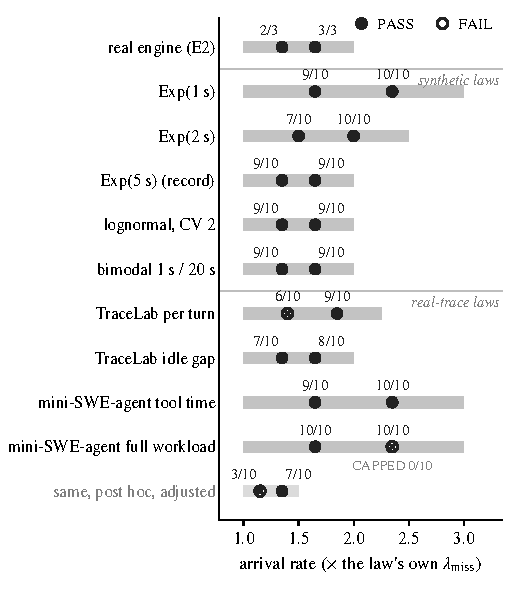
\includegraphics[width=0.94\columnwidth]{figs/fig5_robustness.pdf}
\caption{The paired test across tool-time laws (simulator). Gray bar: from-empty window $[1,\,hi]$ in multiples of each law's $\lmiss$. Markers: test points, filled = pass, crossed = fail (each arm in $\ge7$ of 10 seeds); number = BURST runs trapped of 10. Top row: the real engine (3 seeds, need 2). Bottom row: labelled post-hoc rerun of the mini-SWE-agent full workload.}\label{fig:robust}
\end{figure}

\paragraph{Tool-time laws.} With exponential tool times of mean 1, 2 and 5\,s, a lognormal law (mean 5\,s, coefficient of variation 2) and a bimodal law (80\% at 1\,s, 20\% at 20\,s), $\lmiss$ stays within 0.0718--0.0730\sps: it is a property of the server. Shorter tool times raise the peak ($\mu^*/\lmiss$ is 5.25, 4.57 and 2.97 for means of 1, 2 and 5\,s) and widen the window ($hi=3.0$, 2.5, 2.0); heavy tails at the same mean leave the edge at 2.0. The test passes at all 10 points (Fig.~\ref{fig:robust}): NOBURST and CAPPED succeed in 10 of 10 seeds everywhere, and BURST is trapped in 7 to 10 of 10.

\paragraph{Tool times from real agent traces.} We replaced the tool-time law by empirical tables from SyFI TraceLab, real sessions of two commercial coding agents used by 52 developers \todo{cite TraceLab, arXiv:2606.30560; not in refs.bib} (per-turn mean 8.51\,s with calls capped at 600\,s, median 0.237\,s, coefficient of variation 4.65; and an inter-request idle gap of mean 14.52\,s as an upper bound), and from mini-SWE-agent v2.0.0 on SWE-bench Verified~\citep{jimenez2024swebench} \todo{cite mini-SWE-agent; not in refs.bib} (mean 1.40\,s, median 0.104\,s, coefficient of variation 4.29). $\lmiss$ moved by $-0.8\%$ to $+1.3\%$. The peak moved to $n=32$ (TraceLab per turn) and 40 (idle gap), and a cap at the new peak recovered in 10 of 10 seeds. Eight of the 10 declared points passed, including the two exponential controls. The failure among the primary laws, TraceLab per turn at 1.40 $\lmiss$, is the slope rule: 6 of 10 BURST runs met it, all 10 were stuck at zero hits, and on 20 fresh seeds (post hoc) 17 met it. A secondary workload with mini-SWE-agent's own turn and token counts has sessions that outlive the declared measurement windows ($\lmiss$ is 0.0120\sps{} as declared, 0.0141 with a 20 times longer window); a labelled post-hoc rerun with longer horizons gives a narrower window, $[1,\,1.5]$, and a pass at 1.35.

\paragraph{Burst size and horizon.} At 1.35 and 1.65 $\lmiss$, a burst of 25 sessions never traps (0 of 10), 50 is a coin flip (5 and 6 of 10 trapped), and from 100 up every run is stuck below a hit fraction of 0.2. In runs extended to 30,000\,s after the burst, no trapped BURST run ever returned to a 100\,s window above a hit fraction of 0.5, all 20 ended with 468 to 1065 waiting requests, and no NOBURST run ever exceeded 50.

\paragraph{The slope rule is the fragile part.} Over the 100 BURST runs of the tool-time test the registered rule labels 90 trapped and 10 indeterminate, while all 100 are stuck at zero hits with an all-miss token rate. At 1.35 $\lmiss$ with 20 fresh seeds, 3 are indeterminate (Wilson interval $[0.05,\,0.36]$; median slope $0.77(\lambda-\lmiss)$ against a threshold of 0.5), so the real engine's one in three there is not surprising. Post hoc, a rule on the hit fraction alone would have called all six real BURST runs trapped; we report the registered rule.

\paragraph{The cap must follow the measured curve.} The right cap, 20 for the workload of record at 300k, moves to 32 or 40 with real tool-time laws and to 64--80 with the native pool; a cap above the new peak leaves $(\mu(N),\mu^*)$ open (Proposition~\ref{prop:cap}).

\section{Published mechanisms in the earlier simulator}\label{sec:mech}

\begin{figure*}[t]
\centering
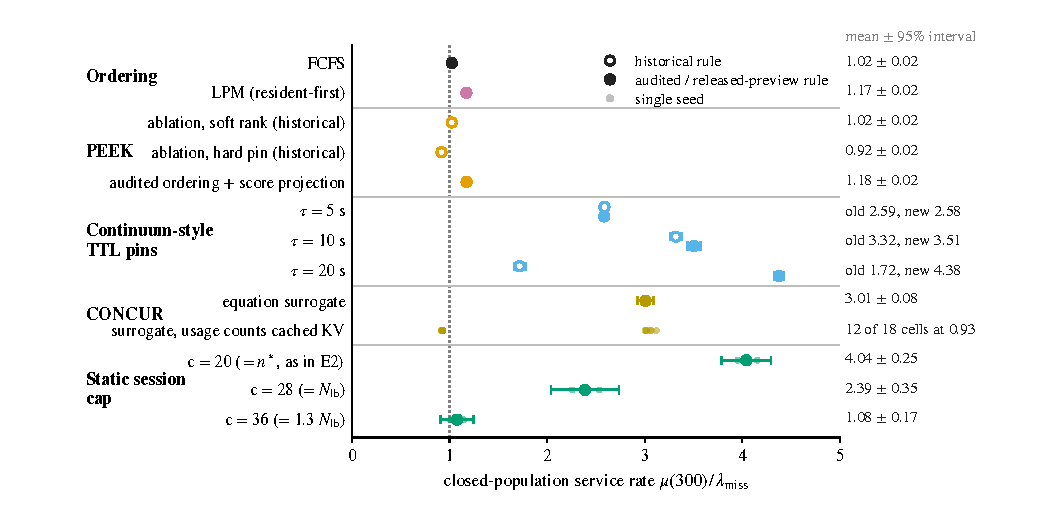
\includegraphics[width=0.92\textwidth]{figs/fig4_mechanisms.pdf}
\caption{$\mu(300)/\lmiss$, our proxy for the congested service rate $\muinf$, per mechanism in the earlier, uncalibrated simulator: mean over 10 seeds with 95\% $t$ intervals, in units of that simulator's $\lmiss$ (0.0474\sps; not comparable with Figs.~\ref{fig:curve}--\ref{fig:edge}); the intervals omit the 1.5\% standard error of $\lmiss$. Hollow: ablations (PEEK's queued-prefix protection under FCFS order, as a soft rank and as a hard-pin counterfactual PEEK does not apply; fixed pins held until expiry even with the GPU idle). Filled: all other rows; for PEEK, a projection of its released scheduler; for the pins, fixed TTLs under the preview's release rule (values: held until expiry, preview). LPM is pure LPM, without SGLang's 128-request fallback. CONCUR: a surrogate of its control equation; small dots: 18 cells in which finished sessions' KV counts as usage. Static caps $c=20$ (E2's cap; this simulator's $n^*$ is 22), 28, 36: $\mu(c)$ of the closed FCFS curve (3 other seeds, not paired with the other rows).}\label{fig:mech}
\end{figure*}

In the fluid model of \S\ref{sec:fluid} the recovery threshold from deep congestion is at most $\muinf$, so a mechanism can raise it only as far as it raises $\muinf$. We compare mechanisms by $\mu(300)/\lmiss$ as a proxy for $\muinf$ (Fig.~\ref{fig:mech}) in the earlier, uncalibrated simulator. Each rule was compared, by reading the code and not running it, with the released code where it exists (PEEK; the Continuum preview, which omits the paper's estimator) or with the paper (CONCUR, for which we found no code); where a difference was small and unambiguous we added a projection of the released rule beside the historical row, and the differences that remain are stated below. That simulator's assumed costs are about 1.5 times the fitted ones ($\lmiss$ 0.0474 against 0.0722\sps), and its curve peaks at 4.07 times its own $\lmiss$, against about 3.0 in the calibrated simulator and $3.26\,\lref$ on the engine. Its absolute rates therefore do not carry over. As in Stage~C, all sessions start at $t=0$, but each run is measured over 25,000\,s after a 5000\,s warmup (static caps: 30,000\,s), about four mean session lifetimes; FCFS reads 1.04 $\lmiss$ over the first half of the window and 1.01 over the second, so the synchronized-start bias of \S\ref{sec:diag} is a few percent here. These are results about the rules in a workload with private prefixes and exponential 5\,s tools, not benchmarks of the named systems.

\paragraph{Orderings.} FCFS gives $1.024\pm0.020$ with hit fraction 0.000 and the GPU always busy; with the 1.5\% standard error of $\lmiss$ included the interval is $1.02\pm0.04$, consistent with Proposition~\ref{prop:A}, which covers this simulator's request-level FCFS. Pure LPM (without SGLang's 128-request fallback) gives $1.174\pm0.023$ and recovers from 300 cold sessions over 150,000\,s up to 1.1 $\lmiss$, not at 1.25. PEEK~\citep{xie2026peek} protects prefixes needed by queued requests and adds a cache-aware scheduler. Our earlier rows implemented only the protection under FCFS order. As a soft ranking, which is how PEEK's eviction hook protects (finite priorities), it gives the same throughput as FCFS seed for seed: queued requests' KV is protected but still evicted before FCFS admits them (2,831--3,128 such evictions per run), so no request is admitted with its KV, consistent with Proposition~\ref{prop:A}. A hard pin, a counterfactual PEEK does not apply, gives 0.919. The released scheduler serves warm requests first; projected onto single-session prefixes with its eviction score, it gives $1.176\pm0.021$, equal to pure LPM within $0.001\pm0.014$, and recovers from none of 5 bursts at 2 $\lmiss$. Here PEEK is an LPM-class ordering, not FCFS; we did not evaluate it on shared-prefix traffic, for which it is designed.

\paragraph{TTL pins.} Continuum keeps a program's KV after a non-final turn for a time-to-live chosen by a cost model, which may be zero~\citep{li2025continuum}. Its released preview omits that estimator: it pins for 2\,s, and only when the parsed tool's historical mean is at most 2\,s, so it would rarely pin our 5\,s-mean tool calls. We did not implement the paper's estimator. Our rows are therefore fixed, unconditional TTLs of $\tau=5$, 10 and 20\,s on every non-final turn, with Continuum's waiting order (pinned programs first). Under the preview's release rule (when an allocation fails and nothing runs, release the pin that expires last) they give $2.584\pm0.035$, $3.505\pm0.064$ and $4.376\pm0.048$; at $\tau=20$\,s the system recovers from a cold start up to 4.0 $\lmiss$ and from 5 of 5 bursts. Under the rule we read in the paper's deadlock-prevention text (when a request does not fit, unpin the latest-arriving programs until it fits, also while work runs), $\tau=10$ and 20\,s give 1.16--1.17 and recover from no cold start at 1.1 $\lmiss$ or above and from no burst. Our earlier rule, which waited for expiry while the GPU idled, gave 1.719 at $\tau=20$\,s. With plain FCFS order instead of Continuum's, under that earlier rule, the pins gave 0.29, 0.17 and 0.10 at $\tau=5$, 10 and 20\,s (3 seeds), with the GPU busy 33\%, 17\% and 8\% of the time: that simulator keeps an expired pin while the session's next request waits, which under FCFS lasts the rest of the queue wait. This is consistent with Proposition~\ref{prop:A}. These are results about configured pins, not about Continuum.

\paragraph{Adaptive caps.} CONCUR adds 2 to a window on active agents when KV usage is below 0.2 and halves it when usage exceeds 0.5 and the hit rate is below 0.2~\citep{chen2026concur}; we found no released code. Our session-gate surrogate of this equation gives $3.009\pm0.081$ and recovers from 5 of 5 bursts. It depends on the usage signal: if finished sessions' KV, still cached and evictable, counts as usage, 12 of 18 cells stall at our surrogate's minimum window of 4 at 0.915--0.935 $\lmiss$; of five exploratory sensitivities, one (a 5\,s control interval instead of our surrogate's 10\,s) raised the rate by $0.184\pm0.167$, an unadjusted pointwise interval. Pause and resume of admitted agents is not modelled. So 3.0 is the surrogate's rate under a live-sessions-only usage signal, not deployed CONCUR's threshold.

\paragraph{Static caps.} By Proposition~\ref{prop:cap} a cap $c$ holds a large population at $\mu(c)$: $4.04\pm0.25$ at $c=20$, $2.39\pm0.35$ at $c=28\approx\Nlb$ and $1.08\pm0.17$ at $c=36$ (3 seeds), against a peak of 4.07 at $n=22$. The cliff makes the choice fragile: a cap about a quarter above $\Nlb$ is back near $\lmiss$.

\paragraph{Admission by memory demand.} ThunderAgent periodically compares the programs' KV demand with the capacity, counting a program in a tool call at a weight that decays with its tool time ($2^{-t}$ in its experiments). When demand exceeds capacity it pauses whole programs, those in tool calls and those with the shortest contexts first, and it restores them when demand falls; both watermarks are set to 1 in its evaluation~\citep{kang2026thunderagent}. NVIDIA Dynamo ships a port that pauses programs at tool boundaries, by default when utilization reaches 0.95 of the pool, down to 0.80, and resumes them at 0.85 or below~\citep{dhanani2026dynamo}. This is an implemented form of a session bound, sized by memory demand rather than count; we have not evaluated it. Proposition~\ref{prop:cap} concerns a FIFO count cap whose sessions keep their slots, so it does not predict a gate that bounds current demand and pauses admitted programs. The static-cap rates above are not a prediction for either system.

\paragraph{Why the ranking comes out this way.} Under request-level FCFS, with or without protection that keeps FCFS order, $\muinf$ cannot exceed $\lmiss$ when (A3) holds (Proposition~\ref{prop:A}); we conjecture (Remark in \S\ref{sec:props}) that pure resident-first orderings raise it through tool calls shorter than the congested lifetime of idle KV, and for pure LPM the simulator agrees. A static cap $c$ holds the engine at $\mu(c)$ (Proposition~\ref{prop:cap}), so at most at the peak, 4.07 at $n=22$ (3 seeds). Pins at $\tau=20$\,s gave 4.38, above every static cap we ran and above the peak, though within the peak's 3-seed interval ($\pm0.36$). In this simulator they also serve pinned programs first and keep a returning session's KV for at least $\tau$, and the set of sessions they bound depends on memory, not on a count; we have not separated these effects. On the real engine, stock LPM recovered from a 200-session burst at 1.35 $\lref$ in 4 of 6 runs (\S\ref{sec:grid}); that finite-burst result does not compare directly with these deep-congestion rates, and in deep congestion stock LPM stops re-sorting its queue, so, on our reading of its source, Proposition~\ref{prop:A} bounds its $\muinf$ by $\lmiss$ when (A3) holds.

\section{A diagnostic, and what it implies}\label{sec:diag}

Choosing the number of admitted jobs from the throughput curve, by paging heuristics~\citep{denning1976optimal} or from measured throughput~\citep{heiss1991adaptive,schroeder2006mpl}, is the classical selection of a multiprogramming level. Stack-distance estimators size a KV tier to the working set, for a target hit rate (KVSET~\citep{li2026kvset}) or for the host offload tier (EfficientAgent~\citep{shao2026efficientagent}), and Yao et al.'s mean-field estimator sizes memory for a target hit ratio when turn gaps are exogenous~\citep{yao2026multiturn}. What the window adds is that the from-empty edge, a finite-horizon stability limit in the sense of Kleinrock and Lam's first exit time~\citep{kleinrock1975aloha}, and not only $\mu^*$, bounds the operating range; that a cap protects against history, not only throughput; and that the right cap moves with the tool-time law, the token profile and the pool.

The window of Eq.~\eqref{eq:window} comes from three measurements that an operator can make before deployment, on the engine, model, pool and workload that will be served. (1) \emph{All-miss capacity}: run a saturated closed population with prefix caching disabled and measure the uncached prefill token rate, which is stable across seeds; check saturation by measuring at two populations (for example 32 and 64 sessions) and use the larger rate, since a population that is not saturated understates $\lmiss$ (our 32-session reference fell about 2--3\% short, \S\ref{sec:props}); convert it to sessions by the mean work per session, or use turns per second over $E[T]$ measured over a window longer than a session's lifetime at that population (mini-SWE-agent's sessions outlived the declared 1800\,s window, and the turn rate there gave a $\lmiss$ 15\% low); completed sessions over a short window are noisy. By Proposition~\ref{prop:A} and the fluid model of \S\ref{sec:fluid}, under request-level FCFS this is an upper bound on the recovery threshold from deep congestion if the congested engine computes prompt tokens no faster than the cache-disabled one, and it equals that threshold if, in addition, $\mu(n)\ge\lmiss$ at every population beyond the peak and not only in the limit (with zero hits, if the engine computes prompt tokens as fast as the cache-disabled one at every congested population); the heuristic work balance of \S\ref{sec:fluid} leads to the same conditions for the open system. With zero hits our engine computed prompt tokens at 1.03 times the all-miss rate near the stationary turn mix and at 0.99--1.12 times it over the windows we measured, so (A3) and (A4) hold on it only to within a few percent at the stationary mix and to within 12\% over those windows. If sessions share a prefix (system prompt, tool definitions), measure instead with caching on and each turn's private context fresh, so that only the shared prefix can hit, the reference against which we expect Proposition~\ref{prop:A} to hold for the private suffixes (\S\ref{sec:props}); disabling caching entirely understates the congested rate. (2) \emph{Closed-population curve}: measure $\mu(n)$ on a grid that crosses the cliff, and do not read $\muinf$ off the largest $n$ of a short run with a synchronized start; here $\mu(300)$ was 0.108\sps, 51\% above $\lref$. (3) \emph{From-empty edge}: run open arrivals from an empty engine at increasing rates over the horizon of interest, at least that of the burst test.

If $\mu^*>\lmiss$, then in the fluid model of \S\ref{sec:fluid}, under request-level FCFS and the assumptions of Proposition~\ref{prop:A}, every operating point in $(\lmiss,\min(\mu^*,\ledge))$ is one sufficiently large burst away from the congested state unless admission is bounded; a steady-state load test there passes without testing recovery. On the engine we tested two rates per pool and one burst size: 200 sessions, about 20 times the 8--12 present at 300k and 6 to 13 times the 16--34 present with the native pool, left all 12 registered SGLang BURST runs at zero hits (11 trapped by the rule); in the simulator 25 never trapped and 50 trapped about half the time. Without a cap, Proposition~\ref{prop:A} and the fluid model predict that recovering from deep congestion requires cutting the arrival rate below $\lmiss$, which was 31\% of peak throughput at 300k tokens and 15\% with the native pool; the earlier, uncalibrated simulator agrees (over 150,000\,s, FCFS recovered from congestion at 0.9 times its own $\lmiss$ and not at 1.0), but no real run lowered the rate after a trap. Stock LPM, which on our reading of its source stops re-sorting its queue when more than 128 requests wait and so falls under Proposition~\ref{prop:A} in deep congestion, recovered from the same finite burst at 1.35 $\lref$ in 4 of 6 grid runs, and at 1.65 $\lref$ in 1 of 6 (\S\ref{sec:grid}); the proposition is a limit statement and does not predict recovery from a finite burst for any ordering. Proposition~\ref{prop:cap} and the quasi-static model suggest a session cap at or just below the peak, since a cap past the peak leaves $(\mu(c),\mu^*)$ open (\S\ref{sec:props}); we take the smallest $n$ within a few percent of the peak (20 at 300k, 64 with the native pool), because the curve has one run per $n$, and check it with a burst test. We recommend a cap because it needs no engine change, its effect in the quasi-static model follows from Proposition~\ref{prop:cap} and Eq.~\eqref{eq:fluid}, and it is the one mechanism we tested on the engine (all 12 registered SGLang CAPPED runs recovered), not because it dominates: in the earlier simulator, 20\,s TTL pins with a pinned-first order reached a higher $\mu(300)$ than any static cap (\S\ref{sec:mech}). A cap does not make the burst free: it moves the burst's cost to the client as admission delay (per-run maxima of 853--985\,s at 300k and 247--361\,s with the native pool), instead of turns that take several minutes for the rest of the run (\S\ref{sec:e2}, \S\ref{sec:e2native}). The delay ends only if the gate drains, which in the quasi-static model needs $\lambda<\mu(c)$ for a cap $c$ (Proposition~\ref{prop:cap} and Eq.~\eqref{eq:fluid}). Whether the gate should queue or reject sessions is a deployment choice we did not evaluate.

The cap must be measured again when the workload or configuration changes. In the simulator the peak moved from 20 to 32 or 40 sessions with the TraceLab tool-time laws and to 24 with mini-SWE-agent's (where the cap stayed at 20), and fell to 12 with mini-SWE-agent's mean turn and token counts. On the real engine it moved to 64--80 with the 955,757-token pool, where the registered cap of 64 drained the burst in every run, and with vLLM 0.32.0 on the 300k pool it stayed at 20--24. A cap sized for one setting can fail in another in either direction. Too small, it holds the engine below the offered load: a cap of 20 under the TraceLab idle-gap law gives $\mu(20)=1.26\,\lmiss$, below both test rates (1.35 and 1.65 $\lmiss$), so the gate would not drain. Too large, it sits on the collapsed side of the curve: with mini-SWE-agent's full workload $\mu(20)$ is 1.45 times that workload's declared $\lmiss$, again below both test rates (1.65 and 2.35). Neither mis-sized cap was run. The procedure sizes a static cap offline and gives no online detector of a trap in progress. Here its three stages took 14--16 A100-hours per pool and engine, and a three-arm burst check about 7.5 more per rate and seed.

\section{Related work}\label{sec:related}

\paragraph{Thrashing, caching and metastability.} The thrashing collapse and the working-set remedy are Denning's~\citep{denning1968thrashing,denning1968working}, and Wilkes analysed the dynamics of paging~\citep{wilkes1973dynamics}; the decomposition analysis of thrashing instability, its stochastic cusp~\citep{nelson1987stochastic,yokohira1989catastrophic} and the choice of a multiprogramming level are classical (\S\ref{sec:background}); LRU's failure on loops is classical~\citep{chou1985evaluation,smaragdakis1999eelru}, as is its weakness on weak-locality patterns~\citep{jiang2002lirs}. Metastable failures were named by Bronson et al.~\citep{bronson2021metastable} and studied in production incidents and modelled by Huang et al.~\citep{huang2022metastable}, whose experiments vary a trigger's magnitude against matched runs and check persistence for an hour after each trigger, the template of our paired test. They were analysed with queueing models, simulation and emulation by Isaacs et al., who also compute a basin for retry storms with a continuous-time Markov chain~\citep{isaacs2025analyzing}, and with continuous-time Markov chains by Alvaro et al.~\citep{alvaro2025formal}; predicted with a queueing model for replicated storage by Habibi et al.~\citep{habibi2024msf}; attributed to destabilizing feedback cycles by Farahbakhsh et al.~\citep{farahbakhsh2025modeling,farahbakhsh2026characterizing}; avoided with bounded concurrency and load shedding in a database simulator by Charapko et al.~\citep{charapko2026execution}; and anticipated with learned indicators by Majumdar et al.~\citep{majumdar2026learning}. An AI system's operating loop has been modelled with cusp bistability and hysteretic recovery~\citep{vanrooyen2026recoverability}. AWS Lambda's container cache can fail to refill once it is empty; Brooker et al.\ also note that a drop in its hit rate raises latency and, by Little's law, the concurrency and working set the cache must hold, relate this to Denning's thrashing, and guard against it with a concurrency limit and cold-start tests at maximum concurrency~\citep{brooker2023ondemand}. Our trap is the case in which the pool is full and rewritten before reuse. Gibbens, Hunt and Kelly's networks with random alternative routing are a classical case in which a state-dependent priority rule, trunk reservation, removes a congested mode and its hysteresis~\citep{gibbens1990bistability}; their modes are both stable, whereas our congested regime is transient, and the closer analogue of our cap is multiprogramming-level load control (\S\ref{sec:background}).

\paragraph{Queueing theory of LLM serving.} Ao et al.\ give fluid-guided scheduling with threshold admission~\citep{ao2025wait} and show that in a decode-only model, which abstracts away prefix reuse, the eviction-free fixed point can be unstable, with rate-limited admission and length mixing as remedies; its benchmark GPU experiments disable prefix caching~\citep{ao2026service}. In its open-arrival simulations, every load tested between the worst-cycle throughput, the analogue of our $\lmiss$, and the eviction-free capacity accumulated backlog. On our engine, backlog accumulated from an empty start only above the from-empty edge; inside our window the good state persisted from empty for the length of each run, and a burst moved the system out of it. Dai et al.\ prove throughput optimality of work-conserving policies without cache state, and give a cyclic-routing example where work-conserving scheduling fails~\citep{dai2025throughput}; Nie et al.\ give stability conditions under KV memory constraints for independent one-shot requests whose KV cache is freed at completion~\citep{nie2026queueing}; Dong and Cao study flow-controlled admission~\citep{dong2026flow}. Dexter et al.\ analyse FCFS and longest-prefix-match scheduling under prefix reuse and latency constraints~\citep{dexter2025prefix}. Yao et al.\ derive a mean-field LRU hit ratio for multi-turn conversations with exogenous gaps between turns, and note that end-to-end latency may change the observed gaps~\citep{yao2026multiturn}; \S\ref{sec:fp-prior} relates our model to theirs and to the Che approximation, whose criterion CacheRoute states for LLM prefix caches and whose single-characteristic-time form it finds misses a 70B engine's hit rate~\citep{cheng2026cacheroute}. In operations research, service systems whose service slows in congestion, or whose customers return, show bistability and are protected by admission control~\citep{chan2014speedup,dong2015slowdowns,ingolfsson2020fluid}; a session that returns after a tool call is such a returning customer, but there the slowdown is a given function of occupancy.

\paragraph{Prefix and KV mechanisms for agents.} PEEK protects prefixes needed by queued requests and adds a cache-aware scheduler~\citep{xie2026peek}; it documents SGLang's 128-request LPM fallback and runs its heavy-load cells at that depth, and its ``scheduling-induced thrashing'' is LPM breaking ties by arrival order. Continuum keeps a program's KV across a tool call for a time-to-live chosen by a cost model, which may be zero, and reports mean tool times of 925\,ms on SWE-Bench (standard deviation 3550\,ms) and 1923\,ms on BFCL~\citep{li2025continuum,patil2025bfcl}. CONCUR controls the number of active agents in closed batch inference with AIMD, halving its window, to exit the thrashing regime, when KV usage exceeds 0.5 and the hit rate is below 0.2, and pausing agents at generation and tool boundaries, reads a sustained low hit rate as a trap, and reports SGLang's hit rate falling from 77.7\% at batch 32 to 35.4\% at 40~\citep{chen2026concur}; MARS sets an admission window by AIMD from GPU KV pressure and CPU tool pressure, and reports that under heavier load its baselines' SLO-aware goodput collapses to near zero while their token throughput stays high~\citep{wang2026mars}. On vLLM, Yuan et al.\ report the prefix-cache hit rate falling from 98.85\% to 16.78\% as the maximum number of concurrent Terminal-Bench agents goes from 15 to 20~\citep{yuan2026agentic}, and VAMP calls the sharp rise in time to first token once reusable prefixes outgrow the KV pool the prefix-cache cliff, and measures stock vLLM at a 0.19\% prefix hit rate on a recorded SWE-bench agent replay~\citep{kim2026vamp}. KAIROS manages GPU frequency and admission for agentic serving under open Poisson arrivals on vLLM and reports context thrashing when its controller lowers the clock or the arrival rate rises~\citep{yuan2026kairos}; AgentKV, from its abstract, prevents the collapse at high concurrency by predictive admission~\citep{anon2026agentkv}; and EfficientAgent's abstract describes state written to the host tier and evicted before reuse by other agents' traffic during tool waits, in a closed pool of agents, where waiting behind other agents lengthens the gap between turns but not the tool waits~\citep{shao2026efficientagent}. ThunderAgent pauses whole programs when their KV demand, with programs in tool calls counted at a weight that decays with tool time, exceeds the capacity, and reports that baseline systems collapse in throughput as the number of parallel workflows grows, a closed population~\citep{kang2026thunderagent}. CacheWise evaluates coding agents with sessions started together~\citep{tiwari2026cachewise}; XPerf, a benchmark, sees hit rates fall toward saturation in fixed-rate runs at increasing rates~\citep{wang2026xperf}. Other systems manage idle KV across tool calls or workflow steps by offloading, prefetching or retention~\citep{abhyankar2024infercept,pan2025kvflow,xia2026mori,bian2025tokencake,zhang2026cachescout,liu2026askthetool,biswas2026sutradhara}, schedule agent programs~\citep{luo2026agentix,lin2024parrot}, cache conversation state hierarchically~\citep{gao2024cachedattention,yu2025pensieve,qin2025mooncake} (Mooncake's scheduler also rejects requests early under overload), admit, place or reserve capacity for agent sessions by tool readiness, KV residency or likely returns~\citep{li2026tao,jiang2026coda,meng2026talaria}, or make locality-aware scheduling fair~\citep{cao2025dlpm}. Eviction-order work~\citep{pan2026rrevict,wu2026randomization,liu2026fancy,pan2026scalesim} changes which idle state is evicted; RR-Evict assumes that the active trajectories fit in the cache, ScaleSim prefetches and evicts each agent's state by the estimated order of the agents' next requests, and Liu et al.\ replay traces without feedback from queueing to arrivals, as do Arya et al.\ for production Microsoft M365 agent traces, where LRU with a pooled budget of a tenth of the busiest hour's no-eviction demand makes 63\% of Deep Research calls recompute~\citep{arya2026residency}. MISA-T, for RL rollouts under a concurrency ceiling, reports vLLM Router's prefix-cache hit rate falling from 92.4\% to 4.5\% at a high ceiling, describes the positive feedback behind it, notes that at prefill saturation the request rate is bounded by prefill throughput over the mean uncached tokens per request, and interrupts the loop with an adaptive admission cap for new sessions derived from observed KV demand and overload pressure~\citep{hong2026misat}; it has no open arrivals, bursts or recovery test. Other close neighbours: Metronome calls a collapse in real-time speech-model serving metastable, in the sense that identical runs collapse or survive near a threshold, but there each session's KV stays pinned for the whole conversation until the pinned KV exhausts the pool, a different mechanism from eviction and recomputation of reusable prefixes~\citep{meng2026metronome}; AgentServeSim simulates agent serving with KV retained across tool gaps and successor turns released by simulated completions, so call timing depends on the policy, and validates it against vLLM in 20 paired cells, without a metastability analysis~\citep{rajib2026agentservesim}; and ServeTwin simulates multi-turn agent workloads while tracking KV-cache evolution and reports that a pool 1.4 times larger lifts the hit rate from 22\% to 93\% at a fixed number of users~\citep{park2026servetwin}.

\paragraph{Position.} The loop is published: under a concurrency ceiling or for a closed population (MISA-T, CONCUR, Yuan et al., VAMP, ThunderAgent~\citep{hong2026misat,chen2026concur,yuan2026agentic,kim2026vamp,kang2026thunderagent}), at fixed concurrency (AgentKV, from its abstract~\citep{anon2026agentkv}), and under open arrivals, where KAIROS reports it after a lowered clock or a higher arrival rate, and a persistent thrashing regime in one uncontrolled run whose clock during the thrashing is not reported~\citep{yuan2026kairos}. Session-aware admission, pausing at tool boundaries and hit-rate thrashing signals are implemented or proposed~\citep{kang2026thunderagent,dhanani2026dynamo,hong2026misat,chen2026concur,wang2026mars,yuan2026kairos,li2026tao,jiang2026coda}. We claim none of these. We add (i) a controlled, replicated, registered test of the open-system claim at a fixed clock and pool, following the trigger design of Huang et al.~\citep{huang2022metastable}: two persistent states at one capacity and offered load, entered by a transient burst, against matched no-burst and capped arms on common random numbers, on two pools and two engines; (ii) the measured sustaining variable, the reuse gap against the pool's turnover time at one load in both states, with a cost-model-free identity for its trapped value (the exact time-domain form of EfficientAgent's backlogged-pool cycle argument~\citep{shao2026efficientagent}); and (iii) a first-principles thrashing curve whose closed forms and out-of-sample predictions were frozen before the H200, Llama, pool, basin and rescue results were read by the agents that derived it (the first author had seen the H200 closed-curve values for $n\le32$, which include the predicted peak). Against the look-aside cases of the metastability literature, where a cache that has lost its contents fails to refill~\citep{bronson2021metastable,huang2022metastable,farahbakhsh2026characterizing}, our pool is full and rewritten before reuse, an instance of what Huang et al.\ call capacity-degradation amplification. Metastability from a unimodal throughput curve, and bounded admission as its cure, are classical (\S\ref{sec:background}). Ao et al.'s decode-only model abstracts away prefix reuse; extending Yao et al.'s model so that the KV held by running requests, and their service time, depend on the hit rate covers our setting, and \S\ref{sec:fp} does this.

\section{Limitations and threats to validity}\label{sec:limits}

\paragraph{One model and GPU, two pools, two engines.} All registered SGLang evidence is for SGLang 0.5.22, Qwen2.5-7B-Instruct and one A100, at two pool sizes: the 300k-token pool limit and the 955,757-token pool SGLang sizes itself. The second answers the concern that the 300k-token pool limit created the cliff: with the native pool the cliff moved out and the registered test passed there too. vLLM 0.32.0 ran only with the 300k-token pool, on the same model and GPU. Its own closed curve and from-empty edge select the same window, $(1,\,2.0)\,\lref$, the same test points, 1.35 and 1.65 $\lref$, and the same cap of 20 as SGLang's 300k cell (\S\ref{sec:vllm}). The exploratory vLLM BURST runs preceded those measurements and had no NOBURST or CAPPED arm, so on their own they cannot exclude that a vLLM NOBURST run would also have congested at these rates within 8700\,s, or that a cap would not have recovered it. The registered vLLM paired test (\S\ref{sec:vllm}) uses the same seeds, reference rate, multiples and burst, so its BURST arm repeats the exploratory runs' workloads and does not replicate them independently. Larger models, parallelism, other GPUs and offloading are untested.

\paragraph{Synthetic sessions and clients.} Sessions are synthetic (random tokens, fixed tool outputs and output lengths, geometric turn counts, exponential 5\,s tools) and share no prefixes, which removes the case PEEK's scheduler targets. These parameters were fixed before we measured any trace, and they differ from the two trace sources of \S\ref{sec:robust}. Our mean tool time of 5\,s lies between theirs (1.40 and 8.51\,s), but their medians are 15--33 times shorter than ours, 63--85\% of their tool times are under 1\,s against 18\% of ours, and their coefficients of variation are 4.3--4.7 against 1. Their outputs per call are 2.7--5.9 times our 100 tokens, and TraceLab's mean prompt, 172k tokens, exceeds our 49,152-token context limit. Apart from one secondary mini-SWE-agent workload, the trace-driven runs of \S\ref{sec:robust} replace only the tool-time law, and only in the simulator. With no shared prefix a miss reuses nothing from other sessions. A shared 2000-token system prompt, cached once, would cut the prompt work of a session from 154,529 to 125,007 tokens when every turn misses and from about 9,600 to 7,600 when every follow-up hits, so the ratio of the two, about 16, would barely change. Production agent traces report a hit rate of about 55\% across turn boundaries and user idle gaps of minutes~\citep{liu2026copilot}, while 93\% of our turns hit in the good state (not the same metric). The simulator suggests that real tool-time laws keep the trap but move the window and the cap; the engine has not tested this. Our clients never retry or abandon a request, and the 7200\,s request timeout never fired, although trapped turns took 163--237\,s on average from send to completion at 300k and 321--511\,s with the native pool. Retries would add load in the trapped state and abandonment would remove it, so either could change whether the engine recovers; neither was tested.

\paragraph{Few runs, finite horizons, nominal rates, uncontrolled factors.} The closed curves and the from-empty sweeps have one run per point, so the peak's location (20 against 24 at 300k and on vLLM, 64 against 80 native) is within noise and single runs near the cliff land on either side of it. The registered tests, the grid and the vLLM runs share the same three seeds, so their runs are not independent across rates, pools or engines (\S\ref{sec:harness}). All rates in this paper are nominal. Each from-empty sweep used a single arrival seed, whose realized rates were 6--13\% above nominal, and in the evaluation windows of the pre-registered SGLang tests the runs labelled 1.35 and 1.65 $\lref$ received 1.27--1.45 and 1.61--1.75 $\lref$ (native, 2.5 and 4.0: 2.48--2.73 and 3.89--4.28; vLLM BURST: 1.24--1.45 and 1.56--1.76). ``Does not leave'' means within 7500\,s on the engine and 30,000\,s in the simulator; the 3000\,s horizon of the from-empty runs cannot see slow escapes, so the true edges may be below 2.0 $\lref$ (both engines) and 5.5 $\lref$ (native). The native cap rests on that coarse curve: $\mu(80)$ was within 0.35\% of $\mu(64)$, and the cliff lies somewhere between 80 and 96 with no run in between. The registered smallest-within-5\% rule gives 64 whichever of 64 and 80 is the true peak (the registration still flags the cap as ambiguous), and with no grid point between 48 and 64 it could not have found a smaller cap; a rule that takes the argmax could as well have picked 80, which may sit within one grid step of the cliff; how far a cap of 64 is from the cliff was not measured. The registered rule loses margin at both ends of the window: the slope test near $\lmiss$, and the token test at high multiples, where the trapped engine's prefill rate rises above the all-miss rate (1.106--1.124 times it at 4.0 $\lref$ with the native pool, against a tolerance of 1.15), so at somewhat higher rates the rule would stop calling a stuck run trapped. In both SGLang closed curves the cliff coincides with a change of job and node (at 300k between $n=32$ and 48, native between 80 and 96; Table~\ref{tab:stages}), so neither curve excludes a node or job effect on where the cliff falls. The collapsed side ran on different nodes in the two curves, which argues against one slow node; on vLLM the hit fraction crossed 0.5 between two runs of one job on one node ($n=28$ and 32); and both registered SGLang tests, which ran on all three nodes with consistent outcomes, argue against a node effect on the trap. The SGLang server seed was not pinned, and the load client runs on the server's node.

\paragraph{Model and simulators.} Eq.~\eqref{eq:fluid} is used only for the window, the recovery threshold and the capped drain time, which the engine met within $-4\%$ to $+52\%$ given the population present at the burst, and it is not quantitative in congestion (\S\ref{sec:fluid}). Proposition~\ref{prop:A} is a limit statement about the closed-population throughput $\mu(n)$ as $n$ grows and says nothing about any finite population. It covers request-level FCFS and, on our reading of the engines' sources, vLLM's FCFS with its preemption and SGLang's stock LPM, which stops re-sorting its queue when more than 128 requests wait; it does not cover program-level FCFS, pure resident-first orders or eviction rules that foresee tool times. It assumes that long-run rates exist, private prefixes, at most one outstanding request per session, no offloading of evicted KV, i.i.d.\ tool times with finite mean that are independent of everything else and unknown to the engine in advance, a bounded number of running requests, a bounded admission rate, and an engine that in congestion computes prompt tokens no faster than with caching disabled; it gives equality only if the engine computes them as fast. With zero hits our engine computed them at 1.03 times the all-miss rate near the stationary turn mix and at 0.99--1.12 times it over the windows we measured, so (A3) and (A4) hold on it only to within a few percent at the stationary mix and to within 12\% over those windows. The proof and Lemma~\ref{lem:waits} were checked by AI review agents and have not been refereed. The open system's recovery threshold rests on a heuristic work balance and, without a monotone tail of $\mu$, can lie below $\lmiss$; that recovery from deep congestion without a cap needs a rate below $\lmiss$ is untested on the engine; pure LPM's congested rate is a conjecture; and the capped system's stochastic stability is not proved. The calibrated simulator failed its level test at $n=48$, reserves whole turns, omits partial prefixes and the refresh, frees a finished session's KV at once (an oracle: a real engine keeps it as evictable cache), and understated LPM. In its primary mode it put the native from-empty edge at least one grid step too high in nominal multiples, against a single real run whose arrivals exceeded the real peak, and for vLLM it predicted a later, gentler cliff than the engine showed (hit fraction 0.46--0.53 against 0.08 at $n=32$). The mechanism comparison uses an older simulator whose assumed costs are about 1.5 times the fitted ones, so its absolute rates and recovery thresholds do not carry over to the engine. Its pin rows are fixed, configured TTLs, not Continuum's cost model; its PEEK rows are ablations and a projection of the released scheduler; and its CONCUR row is a surrogate of the paper's control equation.

\section{Conclusion}\label{sec:conclusion}

Prefix caching turns multi-turn agent serving into a thrashing workload: the cache that makes follow-up turns cheap belongs to sessions idle in tool calls, and admission reclaims it first. In our SGLang configuration the engine stayed in the good state from empty up to twice the all-miss capacity over 3000\,s, and at 1.35 and 1.65 times that capacity the good state was metastable: in a pre-registered test a burst moved the engine into an all-miss state that it did not leave within 7500\,s, the no-burst and capped arms stayed good, and a timing-calibrated simulator had predicted this. Operators should measure the closed-population curve for the workload they serve, cap admitted sessions near its peak, and re-measure when the workload changes.


\section*{Code and data availability}
{\raggedright The repository \repourl{} holds the code (simulator, load generator, analysis and Slurm job scripts), the experiment configurations, the registration files (\fpath{configs/agentload_prereg_*.yaml}), the frozen blind predictions (\fpath{notes/PREDICTIONS*.md}, with their tags), all real-engine data with the job logs (\fpath{results/nova/}), the research log (\fpath{notes/LOG.md}), the scripts behind every figure and derived table, and the source of every number in the paper (\fpath{paper/NUMBERS.md}); this version corresponds to tag \texttt{arxiv-v1}. The directory \fpath{provenance/} holds the archived GitHub push log (\fpath{github_activity_2026-10.json}), which is the external record of when each registration and prediction reached GitHub (\S\ref{sec:prereg}, Appendix~\ref{app:timeline}), the cluster's accounting records of every cited job (\fpath{sacct_cited_jobs_2026-10-30.txt}), and the evidence of the independent verifier of the first prediction round. Simulator outputs are not stored, apart from their summaries; each can be regenerated from the command, commit and configuration recorded with the run (\fpath{meta.json}, \fpath{config.yaml}). The derived tables in \fpath{paper/derived/} name each engine run by its path on the cluster, \fpath{results/agentload_*/<timestamp>}; the run is stored under the pull directory of its jobs in \fpath{results/nova/}, with the same final path components. The agents' tool-call transcripts (\S\ref{sec:sim}, Appendix~\ref{app:timeline}) are not in the repository.\par}

\section*{Use of AI tools}
LLM coding agents (Anthropic Claude through Claude Code, including Claude Sonnet subagents, and OpenAI Codex sessions) were used extensively under the authors' direction. They wrote and tested much of the simulator, load generator and analysis code; prepared and submitted the cluster jobs, under authorizations the first author gave for each experiment or set of experiments; made the blind simulator predictions (\S\ref{sec:sim}); specified the prediction rounds and, afterwards, checked the first round's tool-call transcripts; made, in a separate Codex session, the independent verification of the first round, which reused the prediction agents' copy of the repository rather than a fresh one; audited the citations; read the engine sources, partly through a web tool that returns a language model's summary of each page; checked the model and reviewed the proofs; and drafted and revised the text. The proofs (\S\ref{sec:props}, Appendix~\ref{app:proofs}) were checked by AI review agents and have not been refereed. Every commit, including those the agents made, is recorded under the first author's identity; a history rewrite on 2026-10-22 removed the agents' co-author trailers from commit messages and changed nothing else (\fpath{provenance/commit-map.tsv} maps old hashes to new ones). The authors chose the research question and the experiments and take full responsibility for the content.

\section*{Acknowledgments}
The experiments ran on the Nova cluster at Iowa State University. The research reported in this paper is partially supported by the HPC@ISU equipment at Iowa State University, some of which has been purchased through funding provided by NSF under MRI grants number 1726447 and MRI2018594.

\bibliographystyle{plainnat}
\bibliography{refs}

\clearpage
\appendix
\section{Protocol details}\label{app:protocol}

\begin{table}[htbp]
\centering\footnotesize\renewcommand{\arraystretch}{0.9}
\caption{Real-engine stages (SLURM job IDs on Nova). Submit, start, end and node of every job: \fpath{provenance/sacct_cited_jobs_2026-11-01.txt} (local time; \fpath{_utc.txt}, UTC; see the text).}\label{tab:stages}
\begin{tabular}{@{}l l p{3.6cm}@{}}
\toprule
Stage & Jobs & What it measures\\
\midrule
Stage 0 & 17060165 & smoke test\\
Stage C & 17062103 & closed $\mu(n)$, 300k pool, FCFS, $n\in\{16,20,24,32\}$ (node gpu-1)\\
 & 17062104 & FCFS, $n\in\{48,96,300\}$ (gpu-3)\\
 & 17062105 & LPM, $n\in\{48,300\}$ (gpu-2)\\
E0a & 17072634--37 & $\lmiss$, cache off\\
E0b & 17084750--55 & from-empty stability\\
E2 & 17093387--404 & registered paired test, 2 rates $\times$ 3 seeds $\times$ 3 arms\\
native C & 17096856 & $\mu(n)$, native pool, $n\in\{24,48,64,80\}$ (gpu-2)\\
 & 17096857 & $n\in\{96,128,300\}$ (gpu-1)\\
native E0a & 17096858 & $\lmiss$, native pool\\
grid & 17097086--103 & BURST arm, 3 policy cells\\
vLLM & 17097972--74 & install, GPU check, smoke\\
native E0b & 17100938--39 & from-empty stability, native pool\\
vLLM E0a & 17100940 & $\lmiss$, vLLM, cache off\\
native E2 & 17102173--90 & registered paired test, native pool, 2 rates $\times$ 3 seeds $\times$ 3 arms\\
vLLM BURST & 17102318--23 & BURST arm, vLLM, exploratory\\
vLLM C & 17162959 & $\mu(n)$, vLLM, 300k pool, $n\in\{16,20,24\}$ (gpu-3)\\
 & 17162960 & $n\in\{28,32,40\}$ (gpu-3)\\
 & 17162961 & $n\in\{48,96,300\}$ (gpu-2)\\
vLLM E0b & 17162962--63 & from-empty stability, vLLM\\
vLLM E2 & 17166121--38 & registered paired test, vLLM, 2 rates $\times$ 3 seeds $\times$ 3 arms\\
\midrule
\multicolumn{3}{@{}l}{\emph{Rounds 11 to 14 (Tables~\ref{tab:frozen}--\ref{tab:frozen3})}}\\
H200 & 17166807 & smoke, H200 NVL, 300k pool\\
 & 17166810--13 & E0a and its 64-session check\\
 & 17166818--22 & Stage C, $n=16$--300 (nine runs, with the next row)\\
 & 17166828, 30, 32, 34 & Stage C, the rest of the nine runs\\
 & 17168377--82 & E0b\\
 & 17169668--71 & E0b reseeds, added after 17168377--82 were read (post hoc)\\
 & 17169612--14 & Stage C, $n=36$, 44, 52\\
 & 17169672--80, 82--87 & Stage C, E0b, 600k pool\\
 & 17171020--37 & E2, 600k pool\\
Llama & 17166808 & smoke, Llama-3.1-8B\\
 & 17166814--16 & Stage C\\
 & 17166823, 29, 31, 33 & E0a and its 64-session check\\
 & 17169565--70 & E0b\\
 & 17170409--26 & E2\\
pools & 17168864--81 & Stage C, E0b; 150k, 600k\\
BASIN-1 & 17168500--05 & bursts of 100, then 25\\
E0F & 17168506--07 & from-empty, seeds 3--5\\
LPM-INF & 17168743--45 & BURST, no LPM fallback\\
BASIN-2 & 17169893--901 & bursts of 40, 60, then 50\\
TOOLSLOW & 17169902--07 & $\delta=10$, then 30\,s\\
SHED & 17169908--11 & $\tau=600$, then 3600\,s\\
rescue & 17168965 & smoke test of the gate (never decisive)\\
 & 17168966--71 & R1, 300k pool, 2 rates $\times$ 3 seeds\\
 & 17168972--74 & R4, native pool, 3 seeds\\
\bottomrule
\end{tabular}
\end{table}

\noindent The accounting export \fpath{provenance/sacct_cited_jobs_2026-11-01.txt} was made after the last cited job had ended; its times are Slurm's local time, CDT until 02:00 on 2026-11-01 and CST after it, and \fpath{provenance/sacct_cited_jobs_2026-11-01_utc.txt} gives the same records in UTC. The earlier export \fpath{provenance/sacct_cited_jobs_2026-10-30.txt} covers every job through the vLLM E0b, and the data directories of the vLLM paired test and of the BASIN-1, fresh-seed, rescue, pool-sweep, BASIN-2, TOOLSLOW and SHED jobs hold their own copies (\fpath{sacct_17166121-17166138.txt}, \fpath{sacct_17168500-17168507.txt}, \fpath{sacct_1716896x.txt}, \fpath{sacct_17168864-17168881.txt}, \fpath{sacct_17169893-17169901.txt}, \fpath{sacct_17169902-17169911.txt}).

\begin{table}[htbp]
\centering\footnotesize
\caption{Workload and engines of the real-engine runs.}\label{tab:workload}
\begin{tabular}{@{}l l@{}}
\toprule
First prompt $L_0$ & 2000 tokens\\
Tool output per turn $\Delta$ & 550 tokens\\
Output per turn $d$ & 100 tokens, greedy, \texttt{ignore\_eos}\\
Turns $T$ & $\min(\mathrm{Geometric}(1/15),60)$, $E[T]=14.761$\\
Tool time $Z$ & exponential, mean 5\,s\\
Prompt at turn $k$ & $2000+650(k-1)$ tokens\\
Output feedback & server-returned token ids\\
\midrule
Engine & SGLang 0.5.22, FlashInfer; FA3 on the H200\\
Scheduling & FCFS, waiting-prefix refresh on\\
Batching & chunked prefill 8192, $\le256$ running\\
KV pool & 300,000 tokens; native 955,757\\
 & pool sweep 150,000, 600,000; H200 also 600,000\\
Context limit & 49,152 tokens\\
Model & Qwen2.5-7B-Instruct, rev.\ a09a3545\\
 & one cell: Llama-3.1-8B-Instruct, rev.\ d10aef7\\
 & (NousResearch mirror, shards identical to Meta's)\\
GPU & A100 80GB PCIe, 81,920\,MiB, driver 580.178.04\\
 & two cells: H200 NVL, 143,771\,MiB, same driver\\
\midrule
vLLM & 0.32.0, FCFS (default), prefix caching on\\
 & chunked prefill 8192, $\le256$ running\\
 & 300,000 tokens (18,750 blocks of 16)\\
\bottomrule
\end{tabular}
\end{table}

Table~\ref{tab:workload} lists the workload and engine settings of the real-engine runs.

\paragraph{The sequence of stages.} \emph{Stage~0}, a smoke test of server and client on one GPU, came first; its server logs and those of Stage~C calibrated the simulator (\S\ref{sec:sim}). After E2 we repeated the sequence with the native pool (Stage~C, E0a, E0b, a second registration and \emph{native E2}) and ran an exploratory policy grid. On vLLM we first measured $\lmiss$ and ran the BURST arm alone under an exploratory registration, and later ran its own Stage~C and E0b, a third registration and its paired test (\S\ref{sec:vllm}). An exploratory replication of E0b later used seeds 3--5 at two rates (\S\ref{sec:edge}). Later cells repeat the first stages on an H200 at the same pool and at 600k tokens (\S\ref{sec:h200}), with Llama-3.1-8B, and on the A100 with pools of 150k and 600k tokens; the Llama-3.1-8B and 600k H200 cells have registered paired tests, and registered tests of a rescue (\S\ref{sec:rescue}), of other burst sizes (\S\ref{sec:basin}), of a pause in arrivals and of a tool slowdown follow the paired-test protocol; \S\ref{sec:frozen} lists their frozen predictions and the outcomes in hand.

\paragraph{Stage 0.} The smoke test (job 17060165) verified that every engine flag exists; that cached tokens are reported (a repeated 64-token prompt had 63 tokens cached); that the server returns output token ids; that contexts up to 40,350 tokens are accepted; that the KV pool is exactly 300,000 tokens; that client and server agree on prompt length (0 mismatches over 3191 requests); and that the flush empties the cache (canary 1023 cached tokens before, 0 after).

\paragraph{Stage C and E0a.} Closed population; all sessions start at $t=0$ and a finished session is replaced at once; 900\,s warmup and an 1800\,s measured window; one run per $n$ (seed 0); flush and canary check between runs. The native-pool and vLLM closed curves used the same protocol, with the populations of Table~\ref{tab:stages}. E0a disables the radix cache and runs 32 sessions with seeds 0, 1 and 2, plus 64 sessions with seed 0 as a saturation check. Its per-run values over the window were (sessions/s, turns-based sessions/s, uncached tokens/s): seed 0, 0.0567, 0.0643, 11,076; seed 1, 0.0817, 0.0773, 11,342; seed 2, 0.0767, 0.0730, 11,312; 64 sessions, 0.0544, 0.0676, 11,431. The spread comes from in-flight composition: the mean turn index of the requests in the window was 15.9, 13.2 and 14.1 for seeds 0, 1 and 2. vLLM E0a ran the same protocol with vLLM's prefix caching off: seed 0, 0.0539, 0.0603, 10,208; seed 1, 0.0728, 0.0705, 10,487; seed 2, 0.0700, 0.0662, 10,352; 64 sessions, 0.0467, 0.0631, 10,531.

\paragraph{E0b.} Poisson session arrivals from an empty cache and queue at 1.25, 1.5, 1.75, 2.0, 2.5 and 3.0 $\lref$; one 3000\,s run per rate; stable if the final queue is below 50 and the fitted rise of the queue over the last 1500\,s is at most 10. All runs used arrival seed 0, so they share one random-number stream and the arrivals at each rate are a subset of those at the next higher rate. The six runs received 302, 359, 416, 472, 585 and 697 sessions, 8.3--12.6\% above $\lambda T$ and about 2.1 Poisson standard deviations above it in every run. Native E0b used the same rule at 1.5, 2.5, 3.5, 4.5, 5.5 and 6.5 times the native $\lref$ (361, 587, 811, 1034, 1257 and 1478 sessions, 5.6--11.7\% above $\lambda T$), and vLLM E0b the multiples of the 300k runs of vLLM's $\lref$ (279, 331, 383, 435, 539 and 642 sessions, 8.6--13.3\% above $\lambda T$; stable through 2.0, final queue 81.6 and 247.1 at 2.5 and 3.0).

The fresh-seed E0b (E0F; jobs 17168506--07) repeated 2.0 and 2.5 $\lref$ on the 300k pool with arrival seeds 3, 4 and 5 under the same rule. All six runs were stable, with final queue 0, so the frozen replication rule, which needed 2.0 $\lref$ stable in all three seeds and 2.5 $\lref$ unstable in at least two, is not met. The nominal bracket of 2.0 to 2.5 $\lref$ therefore comes from the single seed-0 grid: over seeds 0 and 3--5, 2.0 $\lref$ is stable in 4 of 4 runs and 2.5 $\lref$ in 3 of 4. Measured instead in realized arrival rates (base arrivals in the 3000\,s run over $3000\,\mathrm{s}\times\lref$), the twelve from-empty runs of seeds 0 and 3--5 are stable up to 2.665 $\lref$ and unstable from 2.726 $\lref$, monotone in the realized rate, so the edge lies between 2.665 and 2.726 $\lref$. The seed-0 run at 2.5 $\lref$ is the one at 2.726: it received 9\% more arrivals than its nominal rate. Either way, the registered rates of 1.35 and 1.65 $\lref$ lie inside the window. The simulator's blind prediction was stable in all six runs; the heuristic H2 of \S\ref{sec:fp-heur} gave each 2.5 $\lref$ run a probability of 0.69 of being unstable and was too pessimistic. This test is exploratory: it has no registration of its own and does not change the E2 registration, whose window was fixed by the seed-0 bracket.

\paragraph{E2.} One arm per 8700\,s job, each on a fresh server; burst of 200 fresh sessions within 60\,s at $t_b=1200$\,s for BURST and CAPPED; CAPPED gate $\ncap=20$; evaluation window $[t_b+4500,\,8700]$\,s. The registered rule (Table~\ref{tab:rule}) was applied by the analysis tool frozen at the registration commit, with the same parameter overrides that the jobs themselves used. Native E2 used the same protocol with the native registration's rates, reference rates and gate $\ncap=64$. Twelve of its 18 runs started after the cluster checkout moved from the registration commit to \texttt{a78ce07}, which adds only the vLLM registration, its input file and two notes files (the research log and the status notes), with no code change, and its verdict ran on that commit; two of its 18 servers sized the pool one token smaller, at 955,756. The vLLM paired test uses the same protocol with the vLLM registration and $\ncap=20$. It uses the same seeds, rates and reference rate as the exploratory vLLM BURST runs, so its BURST arm repeats their workloads rather than replicating them independently.

\paragraph{Why the rule uses tokens.} Criterion (a) uses tokens because a trapped engine with a growing backlog serves mostly young sessions, whose turns are short, so at the all-miss token rate it completes more turns per second than the stationary all-miss mix, and sessions faster than $\lmiss$ (\S\ref{sec:fluid}): on traps simulated in our earlier simulator (\S\ref{sec:sim}), a session-rate test fired on at most 1 of 29 at 2 $\lmiss$ and none of 39 at 2.5, while the token test fired on all 84 traps at 1.5--2.5 $\lmiss$.

\paragraph{Drain-time estimates.} The registrations' feasibility check used $b/(\mu(c)-\lambda)$, which ignores the $c-n_1$ free slots that a burst fills at once: 1571\,s at 1.35 and 1889\,s at 1.65 $\lref$ for E2, 668\,s and 1043\,s at 2.5 and 4.0 $\lref$ for the native test, and 1529\,s and 1800\,s for vLLM. With the populations present at the burst (5--12 sessions at 300k, 11--32 with the native pool, 5--11 on vLLM), the fluid estimate $(n_1+b-c)/(\mu(c)-\lambda)$ of \S\ref{sec:props} is 1453--1508\,s and 1757--1804\,s, 491--518\,s and 840--876\,s, and 1414--1460\,s and 1674--1692\,s. The CAPPED gate's queue emptied 1547--1904\,s and 2021--2693\,s after the burst on E2, 3--52\% longer than this estimate; 512--583\,s and 837--937\,s with the native pool, between 4\% shorter and 13\% longer; and 1521--2735\,s on vLLM, 1.05--1.63 times it.

\paragraph{Rescue (R1, R4).} One rescue run per 8700\,s job, each on a fresh server, from a frozen clone at the registration tag; the client's arrival plan is the BURST plan of the same seed and rate, byte for byte, so until $t_{\mathrm{on}}$ the rescue run replays the BURST run's arrival plan (a fresh run on a fresh server, not the same run). At $t_{\mathrm{on}}$ the gate starts to bind with cap $c$ by attrition and pause: a session whose tool call ends while more than $c$ sessions are admitted gives up its slot and joins a resume queue, which is served before the queue of new arrivals, each in FIFO order; a paused session's KV is not protected while it waits. The cap is removed at the first 10\,s tick at or after $t_{\mathrm{on}}+600$\,s at which both queues have been empty for 300\,s; there is no forced release. The registered per-run rule uses the follow-up hit fraction, the share of a session's turns after its first, attributed by completion time, with more than half of the prompt cached: (a) VALID if the follow-up hit fraction over $[t_{\mathrm{on}}-300,\,t_{\mathrm{on}})$ is below 0.2 and more than 50 requests or sessions are outstanding at $t_{\mathrm{on}}$ (requests in flight plus sessions waiting at the gate or paused), on the registered hardware; (b) RELEASED by 7200\,s; (c) POST-GOOD over $[t_{\mathrm{rel}}+300,\,8700)$: every 300\,s window, tiled from the start with a short remainder covered by the window ending at 8700\,s, has a follow-up hit fraction of at least 0.5, the whole interval above 0.8, an uncached token rate below 0.5 times the all-miss reference, and the registered RECOVERED test holds over the last 300\,s; a window with no completed follow-up fails (c) without being a relapse. RESCUED is (a), (b) and (c); RELAPSE is any such window below 0.2. A same-seed BURST control, from the paired test, is STUCK if its follow-up hit fraction over $[t_{\mathrm{on}},\,8700)$ is below 0.2 and it is not RECOVERED over the last 300\,s. A cell passes if at least 2 of its 3 seeds are RESCUED and every same-seed control is STUCK; R1 is refuted if 2 of its 6 runs relapse or are not released by 7200\,s, and R4 if 2 of its 3 relapse; a refutation takes precedence over a pass, and a failed session in any counted run withdraws the claim that nothing was shed. The pairing requires common random numbers with the committed BURST and NOBURST runs (the BURST plan byte-identical, the NOBURST plan the rescue plan without the burst sessions), equal resolved rates, references, hardware and burst time. Each job ran only a mechanical check of the gate (\texttt{analysis.rescue check-run}: engage within 10\,s of $t_{\mathrm{on}}$, release on the 10\,s grid after the 300\,s hold, no request errors), which passed in all ten jobs; no hit fraction of a rescue run was read before all runs of its cell had ended. The controls ran on 2026-10-24 to 26 as part of the paired tests, not alongside the rescue runs. A smoke job under its own registration checked the gate's mechanics before the registered runs and is never decisive.

\begin{table}[htbp]
\centering\footnotesize
\caption{The registered decision rule.}\label{tab:rule}
\begin{tabular}{@{}l l@{}}
\toprule
Rate estimator & uncached prefill tokens/s\\
Reference rate & E0a all-miss, 11,243 tokens/s\\
 & \quad (native: 11,282; vLLM: 10,349)\\
$\lmiss$ in the rule & the cell's $\lref$\\
Rate tolerance & $\pm0.15$\\
Backlog slope & least squares over 10\,s bin means of\\
 & \quad sessions in the system, gate included\\
Minimum window & 600\,s\\
Trapped & $\lambda>\lmiss$, rate within tolerance,\\
 & \quad and slope $>0.5\,(\lambda-\lmiss)$\\
Recovered & hit $>0.8$ and outstanding $<20$, last 300\,s\\
Draining & slope $<0$\\
Indeterminate & none of the above\\
Precedence & trapped, recovered, draining, indeterminate\\
Hit metric & turns with cached/prompt $>0.5$\\
Pass & $\ge2/3$ of $\ge3$ seeds with all three\\
 & \quad arm conditions met in the seed\\
\bottomrule
\end{tabular}
\end{table}

\paragraph{Backlog definitions.} The figures and Table~\ref{tab:e2} report the backlog as sessions in the system (arrived minus ended), which includes sessions asleep in tool calls (8--12 in the good state at 300k, 16--34 with the native pool). The registered RECOVERED test uses the outstanding backlog (requests in flight plus sessions held at the gate). The simulator's predictions count waiting requests plus the gate queue. The rescue rule's outstanding work also counts sessions paused by the gate (Fig.~\ref{fig:rescue}).

\section{The registrations}\label{app:prereg}
\begingroup\raggedright
The registration was filled by formula from committed copies of the Stage~C curve, the E0a calibration and the E0b bracket. The window was $(1,\,2.0)\,\lref$, its upper edge E0b's largest all-stable multiple (below $\mu^*/\lref=3.26$), a nominal value from E0b's single seed-0 grid; fresh seeds later put the from-empty edge, in realized arrival rates, between 2.665 and 2.726 $\lref$, and both registered points lie inside the stable range on either reading (\S\ref{sec:edge}). The rates followed a rule proposed in the runbook and adopted in the project status notes on 2026-10-22, the day before E0b was submitted (Appendix~\ref{app:prereg}): one third and two thirds of the way across the window, rounded to 0.05, which gives 1.35 and 1.65 $\lref$ (0.0966 and 0.1180\sps). The cap was the smallest $n$ with $\mu(n)\ge0.95\mu^*$: $\ncap=20$, since $\mu(20)=0.224$ is about 4\% below $\mu(24)=0.233$, inside the rule's 5\%. The file was committed and reached the project's GitHub repository at 15:09:54 CDT on 2026-10-24, before the E2 jobs were submitted at 15:13 (Table~\ref{tab:timeline}). We call a test pre-registered when its registration file was committed and pushed to GitHub before its runs; this is not an entry in a third-party registry. Registration and the frozen predictions of \S\ref{sec:sim} are rigor, not a contribution: they let a reader check that each rule and each prediction existed before its outcome. The design follows the model-to-system pipeline of Isaacs et al., in which an abstract model chooses the experiments that then test it~\citep{isaacs2025analyzing}, and pre-registered gates have been used in ML-systems measurement before~\citep{suram2026cacheable}. Appendix~\ref{app:prereg} lists every registration we filled, with its status, and Appendix~\ref{app:timeline} every prediction round with its time record; the files carry no timestamp other than GitHub's push log. The repository we publish is a redacted copy of the development repository whose \fpath{provenance/} directory ties every registration file, by hash chains, to the development repository's push log (availability statement). Commit times are set by the committer, so the external record is GitHub's push log, archived as \fpath{provenance/github_activity_2026-10.json} (Appendix~\ref{app:timeline}). The job script refuses to start unless the file is committed and unmodified and the job's cell, rates, cap, reference rates, hardware and protocol match it, and writes its SHA-256 into every run; the analysis calls a verdict decisive only for the registered cell and rates with every run bound to the file and started after its commit (Appendix~\ref{app:prereg}); the label records this binding, not statistical strength, and the analysis checks commit order, not push time, so its own label ``pre-registered'' does not by itself meet our definition. The native registration was filled and enforced the same way and reached GitHub 10 minutes before its jobs were submitted (\S\ref{sec:e2native}). The vLLM registration was filled from vLLM's own Stage~C curve, E0a calibration and E0b bracket, and does not meet the definition: it was committed 37\,s before its 18 jobs were submitted, and the cluster's record of the submission names the file but not its hash, but it reached GitHub 2\,min after the submission, when two of the jobs had started and none could have ended, so we call this test registered, not pre-registered (\S\ref{sec:vllm}). On the H200 with the 300k pool the rule could not be applied: its window was $(1,\,1.3)\,\lref$ (the largest all-stable E0b multiple, below $\mu^*/\lref=1.99$), and the points the rule gives, 1.10 and 1.20 $\lref$, lie outside the band $(1.1,\,1.17)\,\lref$ that its 10\% margin at each edge of the window leaves, so the fill returned INCOMPLETE and that cell has no registered test (\S\ref{sec:frozen}). With the 600k pool the window was $(1,\,2.5)\,\lref$ and the rule filled a registration (Table~\ref{tab:ledger}).

The registration is \fpath{configs/agentload_prereg_2026-10-24.yaml}, status FILLED, committed in \texttt{d279b7b} at 15:09:12 CDT on 2026-10-24 and pushed to GitHub at 15:09:54, before the E2 jobs were submitted at 15:13:39, SHA-256 \texttt{2a6d680a9615bba962a5673d6db6b3e4\allowbreak ca5102bf778ca974cea46147f5cc0ac6}. Its fields:

\begin{itemize}
\item \textbf{Cell and inputs.} Engine cell \texttt{sglang-fcfs-r1} (SGLang FCFS, waiting-prefix refresh on); committed copies of the Stage~C curve, the E0a calibration and the E0b bracket under \fpath{prereg/inputs/2026-10-23/}; protocol 8700\,s, burst of 200 within 60\,s at 1200\,s.
\item \textbf{Measured.} $\mu(n)$ in sessions/s: 0.1756 ($n=16$), 0.2239 (20), 0.2333 (24), 0.1150 (32), 0.0489 (48), 0.0611 (96), 0.1078 (300). $\mu^*=0.2333$; $\ncap=20$ by the smallest-within-5\% rule (argmax 24; flagged ambiguous). $\lmiss=0.07167$ (sessions) and 0.07153 (turns-based, $=\lref$); all-miss rate 11,243 tokens/s; E0b largest all-stable multiple 2.0, first unstable 2.5, monotone (arrival seed 0 only; the fresh seeds of Appendix~\ref{app:protocol} came later); hardware A100 80GB PCIe.
\item \textbf{Predicted boundaries.} Recovery threshold $\lref$ (not $\mu(300)$, which a synchronized start biases upward). Window $(0.0715,\,0.1431)$\sps{} $=(1.0,\,2.0)\,\lref$, upper edge from E0b. CAPPED drain must fit within 80\% of the 7200\,s available after the burst (5760\,s), which holds for $\lambda$ up to 2.64 $\lref$; predicted drain 1571\,s at 1.35 and 1889\,s at 1.65.
\item \textbf{Rates.} 1.35 and 1.65 $\lref$ by the one-third/two-thirds rule, rounded to 0.05, inside the margin band $(1.1,\,1.8)$; seeds 0, 1, 2. On 2026-10-22 the runbook proposed the rate rule and a cap of 20, with keeping 24 as the alternative (\texttt{288b801}, 13:13 CDT); both rules were adopted in the project status notes at 13:50 (\texttt{4435c51}) and reached GitHub at 17:45, before E0b was submitted on 2026-10-23; the registration's own text dates them 2026-10-23.
\item \textbf{Predictions.} Inside the window: BURST trapped, NOBURST good through the run horizon, CAPPED recovered if the drain fits. Below $\lref$: BURST not trapped. Above the window: NOBURST may escape, so no such rate was registered.
\item \textbf{Kill conditions.} NOBURST not good in at least one third of the seeds at a registered rate; BURST not trapped in two thirds of the seeds at every registered rate; CAPPED not recovering while BURST traps and the drain fits; a window that is empty or narrower than the noise.
\item \textbf{Warnings recorded at filling.} $|\mu(300)/\lmiss-1|=0.507$ (a check only), and the ambiguous cap.
\end{itemize}

\noindent The verdict is in \fpath{results/agentload_analysis_burst2/20261025-144012/} inside the E2 data directory: the registered analysis passes at 1.35 and 1.65 $\lref$ (the tool's labels, assigned by commit order, are pre-registered and decisive; by the definition of \S\ref{sec:prereg} the test is pre-registered). The three grid cells have their own derived registrations, \fpath{configs/agentload_prereg_2026-10-24_grid_<cell>.yaml} for the cells \texttt{sglang-fcfs-r0}, \texttt{sglang-lpm-r1} and \texttt{sglang-lpm-r0}, with status EXPLORATORY; the analysis never calls them decisive.

\paragraph{The native registration.} \fpath{configs/agentload_prereg_2026-10-25_native.yaml}, status FILLED, committed in \texttt{b8c19ec} at 17:31:16 CDT on 2026-10-25 and pushed to GitHub at 17:31:56, 10 minutes before the native E2 jobs were submitted (17:42:29), SHA-256 \texttt{21bf7c03e0630b65b80d086058815e12\allowbreak c5ba9fbe41e9864d3dd0183b9bf776c1}; the same template, formulas, trap rule, kill conditions and protocol as above. Cell \texttt{sglang-fcfs-r1-native}; inputs under \fpath{prereg/inputs/2026-10-25-native/}. Measured: $\mu(n)$ 0.2650 ($n=24$), 0.4311 (48), 0.4789 (64), 0.4772 (80), 0.1228 (96), 0.0667 (128), 0.1006 (300); $\mu^*=0.4789$; $\ncap=64$ by the smallest-within-5\% rule (also the argmax; flagged ambiguous, $n=80$ within 0.35\%); $\lref=0.07180$ (turns-based); all-miss rate 11,282 tokens/s; native E0b largest all-stable multiple 5.5, first unstable 6.5, monotone. Window $(0.0718,\,0.3949)$\sps{} $=(1,\,5.5)\,\lref$, upper edge from native E0b, below $\mu^*/\lref=6.67$. Rates 2.5 and 4.0 $\lref$ (0.1795 and 0.2872\sps) by the same rule, inside the margin band $(1.1,\,4.95)$; the rule was recorded in the project status notes (\texttt{6cb43e9}, pushed 15:08 CDT) before native E0b was read. Predicted drains 668\,s and 1043\,s; the drain fits up to 6.19 $\lref$. Warnings recorded at filling: $|\mu(300)/\lmiss-1|=0.401$, the ambiguous cap, and an incomplete grid (no $n=16$, 20 or 32). The verdict is \fpath{results/agentload_analysis_burst2/20261026-100653/} inside the native E2 data directory: the registered analysis passes at 2.5 and 4.0 $\lref$ (with the same tool labels; pre-registered by the definition of \S\ref{sec:prereg}).

\paragraph{The exploratory vLLM registration.} \fpath{configs/agentload_prereg_2026-10-24_grid_vllm-fcfs.yaml}, status EXPLORATORY, derived from the E2 registration, committed in \texttt{a78ce07} at 18:06:18 CDT on 2026-10-25 and pushed to GitHub at 18:06:33, 46\,s before the vLLM BURST jobs were submitted, SHA-256 \texttt{c5037cac6003c4e98da89f88dae953bf\allowbreak e68bb21a27a4e3e5e3dab3c8891aeab5}. Cell \texttt{vllm-fcfs}, BURST arm only; the window, multiples, protocol and trap rule are inherited from \texttt{sglang-fcfs-r1}, and the reference rates come from \fpath{prereg/inputs/2026-10-25-vllm/calibration.json}, a byte-identical copy of the vLLM E0a calibration. Its predicted-boundary block is copied unchanged from the E2 registration (window 0.0715--0.1431\sps, all-miss rate 11,243 tokens/s), but the runs used vLLM's references, 0.06566\sps{} and 10,349 tokens/s (\texttt{lambda\_ref\_resolved} and \texttt{uncached\_tokens\_ref\_resolved} in each run's \fpath{meta.json}), so their rates were 1.35 and 1.65 times vLLM's $\lref$. The verdict, \fpath{results/agentload_analysis_burst2/20261026-100701/} inside the native E2 and vLLM BURST data directory, reports per-run states and no registered verdict.

\paragraph{The vLLM registration.} \fpath{configs/agentload_prereg_2026-10-30_vllm.yaml}, status FILLED, SHA-256 \texttt{8f2d5b44d6365795fedde8bf673d51e5\allowbreak 4bf8a685a14d563c86de44492bb95f84}; the same template, formulas, trap rule, kill conditions and protocol as the E2 registration. Cell \texttt{vllm-fcfs}; inputs: the vLLM Stage~C curve and E0b bracket under \fpath{prereg/inputs/2026-10-30-vllm/}, byte-identical to the analyses in the vLLM Stage~C and E0b data directories, and the vLLM E0a calibration above. Measured: $\mu(n)$ 0.1750 ($n=16$), 0.2194 (20), 0.2183 (24), 0.1189 (28), 0.0433 (32), 0.0411 (40), 0.0439 (48), 0.0572 (96), 0.1050 (300); $\mu^*=0.2194$; $\ncap=20$ by the smallest-within-5\% rule (also the argmax; flagged ambiguous, $n=24$ within 0.5\%); $\lref=0.06566$ (turns-based); all-miss rate 10,349 tokens/s; vLLM E0b largest all-stable multiple 2.0, first unstable 2.5, monotone. Window $(0.0657,\,0.1313)$\sps{} $=(1,\,2.0)\,\lref$, upper edge from vLLM E0b, below $\mu^*/\lref=3.34$. Rates 1.35 and 1.65 $\lref$ (0.0886 and 0.1083\sps) by the same rule, inside the margin band $(1.1,\,1.8)$; this rule and the cap rule were recorded in the project status notes (\texttt{836063a}, pushed 12:16 CDT on 2026-10-30) after the vLLM Stage~C and E0b jobs were submitted and before any of them had ended. Predicted drains 1529\,s and 1800\,s; the drain fits up to 2.81 $\lref$. Warnings recorded at filling: $|\mu(300)/\lmiss-1|=0.599$ and the ambiguous cap. The file was filled from five of the six vLLM E0b runs while the 3.0 $\lref$ run was still running; with 2.5 $\lref$ unstable that run could not change the edge, and it was unstable too, so the six-run bracket equals the registered one. The file was committed in \texttt{5a6fbcd} at 16:23:59 CDT, 37\,s before the 18 jobs of the paired test (17166121--38) were submitted at 16:24:36 (the research log gives 16:30), and the jobs run from the cluster's copy of the repository at that commit; Slurm's record of the submission names the file but not its hash. It reached GitHub at 16:26:35, 1\,min 59\,s after the submission, when two of the jobs had started (at 16:25:42 and 16:26:17) and none could have ended. This registration therefore does not meet the definition of \S\ref{sec:prereg}: it was committed before the jobs were submitted, but pushed after the first two had started, so we call this test registered, not pre-registered. As for E2, the job script writes the file's SHA-256 into every run's \fpath{meta.json}.

The verdict, \fpath{results/agentload_analysis_burst2/20261031-020837/} in the paired test's data directory (\fpath{results/nova/e2_vllm_1716612x_pulled_20261031-020956/}), reports a pass at both rates; all 18 runs' \fpath{meta.json} files carry the registration's SHA-256. The tool also prints the labels pre-registered and decisive, which it assigns by commit order; by the definition of \S\ref{sec:prereg} the test is registered, not pre-registered. The frozen mechanism predictions for this test (\fpath{configs/r11_mechanism_predict.yaml}, \fpath{notes/PREDICTIONS_r11_mechanism.md}; commit \texttt{f1338e3}, pushed at 18:20:13 CDT on 2026-10-30, when three of the 18 jobs were running and none had ended; the first ended at 18:55:07) were evaluated with the frozen scripts, run unchanged. Byte copies of the frozen files and their outputs are under \fpath{r11_mechanism/} in the same directory, and the scored decision is \fpath{derived/r11_mechanism_decision.json}, which records two detector false alarms in CAPPED runs, one more than the frozen rule allows (\S\ref{sec:vllm}).

\paragraph{The rescue registrations.} \fpath{configs/agentload_prereg_2026-10-31_rescue.yaml} (R1, cell \texttt{sglang-fcfs-r1-rescue}) and \fpath{configs/agentload_prereg_2026-10-31_rescue_native.yaml} (R4, cell \texttt{sglang-fcfs-r1-rescue-native}), status FILLED, SHA-256 \texttt{502dee9e3107952a2f968c1b59b8ee3d\allowbreak 4063870d72f0dfac1261e2b2e2316691} and \texttt{ddd776f822755ba50472668b4af7dba3\allowbreak 538354d98feb2579b8cca422b5215bb1}, were committed in \texttt{f0bc3ad} at 22:10:47 CDT on 2026-10-30 (tag \texttt{r11-rescue-reg}) and reached GitHub at 22:39:02, 22 minutes before the ten jobs (a smoke job and the nine registered runs, 17168965--74) were submitted at 23:01:12--13; by the definition of \S\ref{sec:prereg} both tests are pre-registered. They reuse the inputs, rates and caps of the E2 and native E2 registrations, under their own cell labels, and add the rescue protocol, the per-run rule, the decision rule and the refutation conditions of Appendix~\ref{app:protocol}, with the rule's constants frozen in \fpath{analysis/rescue.py} at the tag. Three changes were accepted after a review of the simulator's predictions and before any rescue run: a refutation takes precedence over a pass, the no-shed part of a pass is withheld if any counted run has failed sessions, and R4, like R1, requires stuck same-seed BURST controls. R4's engage time of 2100\,s replaced 2400\,s after the simulator had predicted 13 of 20 rescued at 2400\,s (\fpath{notes/PREDICTIONS_r11_rescue.md}). The verdicts, \fpath{results/agentload_analysis_rescue_r1/20261031-071720/} and \fpath{results/agentload_analysis_rescue_r4/20261031-071748/} in the data directory \fpath{results/nova/rescue_1716896x_pulled_20261031-070502/}, were computed on a clean tree with the registrations and the simulator's predictions as inputs: each reports a pass, with no rejected run and no pairing, protocol or registration problem, and every run's \fpath{meta.json} carries its registration's SHA-256. The tool labels each verdict decisive, a label it assigns by commit order.

\paragraph{Ledger of registrations.} Table~\ref{tab:ledger} lists every registration file we filled, with its status. Commit times are the committer's; push times come from GitHub's push log (\fpath{provenance/push_times_2026-11-01.tsv}, built from the export of 2026-11-01, or the archived log itself for the grid cells). Each is the first branch update that contains the commit; the BASIN-1 push also carried \texttt{9b67c26}, the commit of tag \texttt{r11-basin-reg}.
\par\endgroup

\begin{table*}[tbp]
\centering\footnotesize
\caption{Every registration, in order. FILLED registrations bind a test's cell, rates, cap, references, hardware and protocol, and the job script refuses to run a test without one; EXPLORATORY ones are derived from a FILLED parent and are never called decisive. Times CDT.}\label{tab:ledger}
\begin{tabular}{@{}>{\raggedright\arraybackslash}p{5.0cm} l l >{\raggedright\arraybackslash}p{2.2cm} >{\raggedright\arraybackslash}p{4.0cm}@{}}
\toprule
File (\fpath{configs/agentload_prereg_*}) & status & committed & on GitHub & runs and outcome\\
\midrule
\fpath{2026-10-24.yaml} (E2) & FILLED & \texttt{d279b7b} 10-24 15:09:12 & 15:09:54 & 18 runs; pass (\S\ref{sec:e2})\\
\fpath{2026-10-24_grid_sglang-*.yaml} (3 grid cells) & EXPLORATORY & \texttt{499c0df} 10-24 23:30:55 & 23:31:32 & 18 BURST runs (\S\ref{sec:grid})\\
\fpath{2026-10-25_native.yaml} (native E2) & FILLED & \texttt{b8c19ec} 10-25 17:31:16 & 17:31:56 & 18 runs; pass (\S\ref{sec:e2native})\\
\fpath{2026-10-24_grid_vllm-fcfs.yaml} & EXPLORATORY & \texttt{a78ce07} 10-25 18:06:18 & 18:06:33 & 6 BURST runs (\S\ref{sec:vllm})\\
\fpath{2026-10-30_vllm.yaml} (vLLM E2) & FILLED & \texttt{5a6fbcd} 10-30 16:23:59 & 16:26:35, after two jobs started & 18 runs; pass; registered, not pre-registered\\
\fpath{2026-10-30_b100.yaml}, \fpath{_b25.yaml} (BASIN-1) & FILLED & \texttt{9128995} 10-30 19:51:20 & 20:04:30 & 6 BURST runs; pass (Table~\ref{tab:frozen2})\\
\fpath{2026-10-30_grid_sglang-lpminf.yaml} & EXPLORATORY & \texttt{5064580} 10-30 21:02:19 & 21:02:46 & 3 BURST runs; no collapse on the two informative seeds, no recovery (Table~\ref{tab:frozen3})\\
\fpath{2026-10-31_rescue.yaml} (R1), \fpath{_rescue_native.yaml} (R4), \fpath{_rescue_smoke.yaml} & FILLED & \texttt{f0bc3ad} 10-30 22:10:47 & 22:39:02 & 9 runs, submitted 23:01; R1 and R4 pass (\S\ref{sec:rescue}); the smoke job is never decisive\\
\fpath{2026-10-31_b40.yaml}, \fpath{_b50.yaml}, \fpath{_b60.yaml} (BASIN-2) & FILLED & \texttt{621d88f} 10-31 01:58:38 & 02:10:48 & 9 runs, submitted 04:21; bracketed: 40 good, 60 stuck, 3 of 3 each (\S\ref{sec:basin})\\
\fpath{2026-10-31_toolslow_d10.yaml}, \fpath{_d30.yaml} & FILLED & \texttt{b006291} 10-31 02:27:40 & 02:28:09 & 6 runs, submitted 04:21; rule not met: 10\,s good in 3 of 3, 30\,s stuck in 1 of 3 (\S\ref{sec:frozen})\\
\fpath{2026-10-31_shed_t600.yaml}, \fpath{_t3600.yaml} & FILLED & \texttt{b006291} 10-31 02:27:40 & 02:28:09 & 4 runs, submitted 04:21; pass: 600\,s stuck, 3600\,s good, 2 of 2 each (\S\ref{sec:frozen})\\
H200 cell, 300k pool & none & & & window $(1,\,1.3)\,\lref$ too narrow: the rule's rates 1.10 and 1.20 fall outside its margin band $(1.1,\,1.17)$, and the fill returns INCOMPLETE; no test\\
\fpath{2026-10-30_llama31.yaml} (Llama-3.1-8B E2) & FILLED & \texttt{1559f8e} 10-31 07:49:13 & 07:49:15 & 18 runs, submitted 07:50:02 (17170409--26); window $(1,\,2.0)\,\lref$, 1.35 and 1.65 $\lref$, cap 20; pass at 1.65 $\lref$, fail at 1.35 (\S\ref{sec:frozen})\\
\fpath{2026-10-31_h200_p600k.yaml} (H200 600k E2) & FILLED & \texttt{4d1d431} 10-31 09:26:38 & 09:26:41 & 18 runs, submitted 09:27:44 (17171020--37); window $(1,\,2.5)\,\lref$, 1.5 and 2.0 $\lref$, cap 48; pass at both rates (\S\ref{sec:frozen})\\
\bottomrule
\end{tabular}
\end{table*}

\noindent Superseded before registration: a native rescue engaged at 2400\,s, whose simulator prediction (13 of 20 rescued) led to the engage time of 2100\,s that R4 registers (\fpath{notes/PREDICTIONS_r11_rescue.md}). The SHA-256 of every tagged file is in its tag message (\texttt{r11-basin-reg}, \texttt{r11-lpminf-pred}, \texttt{r11-rescue-reg}, \texttt{r14-basin2-reg}, \texttt{r14-extra-reg}) and in \fpath{provenance/registration-proofs/}; the Llama-3.1-8B and 600k H200 registrations are not tagged, and the job script writes their SHA-256 into each of their runs' \fpath{meta.json}.

\section{Prediction rounds and timeline}\label{app:timeline}

\paragraph{The calibrated simulator in detail.} Our discrete-event simulator models a continuous-batching engine: iterations of at most 8192 prefill tokens and 256 sequences; admission reserves a request's end-of-turn KV; idle KV of sessions in a tool call or waiting is evicted whole, least recently used first; waiting requests pin nothing; a finished session's KV is freed at once, an oracle, since a real engine keeps it as evictable cache. An iteration costs a fixed time plus a per-token term plus attention terms. The five cost parameters were fitted only to SGLang's per-batch timing lines in the Stage~0 and Stage~C server logs (decode $R^2=0.992$, median error 0.75\%; prefill $R^2=0.998$, 1.3\%), never to $\mu(n)$. It runs mixed prefill--decode iterations or, like SGLang, separate iterations with prefill priority; the primary (mixed) mode was the one closer to the real Stage~C $\mu(n)$ under a pre-declared metric (mean relative error 0.104 against 0.127), a margin carried by one cell, and both modes' predictions are reported. It does not model partial prefixes, the waiting-prefix refresh or the overlap scheduler; reserving whole turns at admission is an upper bound on what paged engines hold (in round 5 of the earlier simulator, on-demand allocation with preemption and SGLang-like ratio reservation kept the curve and the trap).

\paragraph{Validation.} The declared level test, simulated $\mu$ within 15\% of the real value in each of 8 Stage~C cells, failed in both modes: mixed batching missed one cell, FCFS $n=48$, by $+42\%$ (0.070 against 0.049\sps), separate batching two. The shape was reproduced: the hit fraction crosses 0.5 at $n=32.5$ against 32.2, the plateau ($n=16$--24) agrees within 9.2\% and $n=300$ within 2\%, and $\mu(300)/\mu^*$ is 0.50 against 0.46. The single real run at $n=48$ dipped below the simulator's all-miss level; its turns-based estimate, 0.063\sps, is within 15\%. Keeping a finished session's KV as evictable cache, a labelled sensitivity arm, left mixed batching the closer mode (0.118 against 0.146) but lowered the plateau ($-15.5\%$ at $n=24$; 5 of 8 cells within 15\%). In the earlier simulator the same change moved the orderings and pins of \S\ref{sec:mech} by at most 0.025 $\lmiss$ but stalled the CONCUR surrogate at its minimum cap in 12 of 18 cells; the static caps were not rerun.

\paragraph{Prediction rounds.} The calibrated simulator then predicted, in both modes (mixed primary), B1: $\lmiss$ and the all-miss token rate; B2: the fraction of from-empty runs that stay stable at each rate; B3: the E2 outcome at each rate from 0.09 to 0.16\sps; B4: the closed curve with 600k- and 900k-token pools. Two later rounds repeated these predictions for the native pool (B1n--B4n) and for vLLM (B1v--B4v, with the simulator's token costs scaled to vLLM's measured all-miss rate, a fit, not a prediction), and three more, for the tests of \S\ref{sec:frozen}, were made by the same simulator (rounds 11 and 12) and by the first-principles model of \S\ref{sec:fp} (round 13, in two sets: tag \texttt{r13-theory-pred}, and \texttt{r13-theory-pred2} for BASIN-2, TOOLSLOW, SHED and the H200 600k cell, with the pool-sweep lookups and the rival scoring of the 0.5-hit crossing used for the pool sweep, the 300k H200 and Llama-3.1-8B). LLM coding agents made the simulator predictions, each in its own copy of the repository and instructed not to read the results they predicted; every round was committed and pushed under a tag before its results were read by its authors. What that means differs by round: B3, B4 and B3n are blind in time; B2 was pushed after E0b had finished on the cluster but before its results were pulled, and B2n, B2v and B4v after their jobs were submitted but before any had finished; B1, B1n and B4n are not blind, and B1 is close to the calibration data; B3v predates the vLLM registration, but its BURST part is blind only on the predicting agent's side. An independent verifier reran the first round. Appendix~\ref{app:timeline} gives the details and the time record of every round.

\begin{table}[p]
\centering\footnotesize
\caption{Order of events, 2026-10-21 to 10-26 (times CDT). Commits are those of the development repository (availability statement); commit and tag times are recorded by the committer, push times by GitHub's activity log, job times by Slurm.}\label{tab:timeline}
\begin{tabular}{@{}p{1.75cm} >{\raggedright\arraybackslash}p{5.6cm}@{}}
\toprule
When & Event\\
\midrule
10-21 & Stage 0 passes (17060165); Stage C submitted 15:28 (17062103--05)\\
10-22 12:54 & Stage C results pulled\\
10-22 13:13 & runbook proposes the rate rule and a cap of 20 (\texttt{288b801})\\
10-22 13:14 & E0a submitted (17072634--37); the last job ends 16:34\\
10-22 13:50 & rate rule and cap adopted in the status notes; simulator cost model fitted to Stage 0/C server logs (\texttt{4435c51})\\
10-22 17:03 & Stage 0 and C data committed (\texttt{d0235a7})\\
10-22 17:45 & first push to GitHub, with the three commits above\\
10-23 14:32 & E0a results committed (\texttt{a76f5e5})\\
10-23 14:42 & E0b submitted (17084750--55); jobs end by 16:09\\
10-24 03:13 & validation of the calibrated simulator committed (\texttt{813cfc1})\\
10-24 03:23 & prediction spec and code committed before any prediction run (\texttt{630ab9e}); on GitHub 03:24\\
10-24 03:49 & predictions B1--B4 committed (\texttt{64bc4e3})\\
10-24 04:05 & independent verification recorded (\texttt{877b936})\\
10-24 14:52 & tag \texttt{r6-predictions-frozen} (tagger time)\\
10-24 14:53 & B1--B4 and the verification reach GitHub\\
10-24 15:06 & E0b results pulled\\
10-24 15:09 & E0b data and registration committed in the same second (\texttt{cfbc702}, \texttt{d279b7b}); registration on GitHub 15:09:54\\
10-24 15:13 & E2 submitted (17093387--404)\\
10-24 15:38 to 10-25 02:36 & E2 jobs run\\
10-25 02:28 & native-pool Stage C and E0a start (17096856--58)\\
10-25 14:40 & registered E2 verdict computed (data \texttt{49fbc7b})\\
10-25 14:42 & native Stage C curve analysed on the cluster; native curve and $\lmiss$ in the status notes at 14:47 (\texttt{6793fb7})\\
10-25 14:45 & native E0b (17100938--39) and vLLM E0a (17100940) start\\
10-25 14:49 & native prediction spec committed (\texttt{29728e3})\\
10-25 14:52 & native Stage C and E0a data committed (\texttt{fa265c2})\\
10-25 14:54 & B1n--B4n run on the clean code commit \texttt{0336c91}\\
10-25 15:06 & B1n--B4n committed (\texttt{e3ea48f}); on GitHub 15:08:28\\
10-25 15:08 & tag \texttt{r8-native-predictions-frozen} (tagger time); native rate rule in the status notes (\texttt{6cb43e9})\\
10-25 17:26 & native E0b jobs end; pulled 17:30\\
10-25 17:31 & native E0b data and native registration committed (\texttt{f3f55ab}, \texttt{b8c19ec}); registration on GitHub 17:31:56\\
10-25 17:42 to 10-26 01:11 & native E2 jobs (17102173--90)\\
10-25 18:06 & vLLM calibration and exploratory registration committed (\texttt{65b65e2}, \texttt{a78ce07}), on GitHub 18:06:33; vLLM BURST submitted 18:07 (17102318--23)\\
10-25 22:42 to 10-26 03:24 & vLLM BURST jobs\\
10-26 10:07 & native E2 and vLLM BURST verdicts computed (data \texttt{f116cf3})\\
\bottomrule
\end{tabular}
\end{table}

\begin{table}[htbp]
\centering\footnotesize
\caption{Order of the vLLM events on 2026-10-30 (times CDT, recorded as in Table~\ref{tab:timeline}).}\label{tab:timeline-vllm}
\begin{tabular}{@{}p{1.75cm} >{\raggedright\arraybackslash}p{5.6cm}@{}}
\toprule
When & Event\\
\midrule
12:10 & vLLM Stage C (17162959--61) and E0b (17162962--63) submitted; 17162959--60 start 12:11\\
12:16 & rule for the vLLM cap and rates in the status notes, on GitHub (\texttt{836063a})\\
12:31 & B1v--B4v committed (\texttt{cc01dbf}); tag \texttt{r9-vllm-predictions-frozen} 12:32 (tagger time)\\
12:32 & B1v--B4v reach GitHub (12:32:44)\\
14:36 & first vLLM jobs end (Stage C, 17162959--60)\\
15:35 & vLLM Stage C curve analysed on the cluster\\
16:23 & bracket of the five finished vLLM E0b runs (16:23:19); vLLM registration committed (\texttt{5a6fbcd}, 16:23:59)\\
16:24 & paired test submitted (17166121--38, 16:24:36); first job starts 16:25:42, second 16:26:17\\
16:26 & vLLM registration and Stage C data (\texttt{276c5f0}) reach GitHub (16:26:35)\\
17:17 & vLLM E0b job 17162963, with the 3.0 $\lref$ run, ends\\
17:28 & vLLM E0b data committed and pushed (\texttt{582c2a6})\\
\bottomrule
\end{tabular}
\end{table}

\noindent Commit and tag times are set by the committer. The external record is GitHub's activity log for the development repository, archived in \fpath{provenance/github_activity_2026-10.json} and, refreshed after the last registered job, \fpath{provenance/github_activity_2026-11-01.json}, together with the cluster's accounting records of the cited jobs (\fpath{provenance/sacct_cited_jobs_2026-10-30.txt}, \fpath{provenance/sacct_cited_jobs_2026-11-01.txt}). The development repository is private; the archived log is an unsigned export made by the first author with GitHub's API, and the hash chains in \fpath{provenance/registration-proofs/} show that the files are unchanged, not when they were pushed; \fpath{provenance/push_times_2026-10.tsv} and its refresh \fpath{provenance/push_times_2026-11-01.tsv}, which adds the rounds 11 to 14, list, for each registration and prediction commit, its first arrival on GitHub and the first job it concerns. GitHub records no push time for tags, so the push times given here are those of the first branch update that contains each commit. The branch holding B1--B4 (\texttt{64bc4e3}) and the verification reached GitHub at 14:53:07 CDT on 10-24, and the E2 registration (\texttt{d279b7b}) at 15:09:54, before the E2 jobs were submitted at 15:13:39. On 10-25, B1n--B4n (\texttt{e3ea48f}) arrived at 15:08:28, the native registration (\texttt{b8c19ec}) at 17:31:56 and the exploratory vLLM registration (\texttt{a78ce07}) at 18:06:33. Pull times are from our local records only.

B3 (E2) and B4 (native pool) reached GitHub before their experiments were submitted, so they are blind in time. B2 (E0b) was committed after E0b had finished on the cluster but before its results were pulled. The LLM agents that made the predictions worked in separate copies of the repository at a commit without the E0a or E0b results and were instructed not to contact the cluster and not to open the E0a or E0b result directories or the primary copy of the repository; they could technically have done so. Their tool-call transcripts, which are not in the repository, were checked afterwards by the orchestrating Claude Code session, which found no cluster command and no access to E0b before the predictions reached GitHub. For B2 this instruction-level control, checked after the fact, is the only safeguard. A scan of every line added between the commit the agents started from and the predictions found no use of withheld data, but a text scan cannot prove that nobody read it. B1 (E0a) rests on the same instruction only: E0a was committed before the predictions. The independent verifier, a separate OpenAI Codex session, had read the project status notes, which mention E0a, so it is independent but not blind; it also reused the prediction agents' copy of the repository instead of a fresh one, as its record states. Its evidence is in \fpath{provenance/codex_prediction_verification/}. Two conditions of the verification failed and are disclosed: the strict containment of B3 passes within the B2 all-stable range, and the platform-specific test failures of the full suite.

In the second round, B2n (native E0b) and B3n (native E2) reached GitHub while native E0b was still running, before any of its runs had finished, and before the native registration or any native E2 job existed. B3n is therefore blind in time. B2n reached GitHub 23\,min after the two native E0b jobs were submitted, when both were running, so it is blind in the sense that no result existed, not in submission order. B1n and B4n are not: native Stage C and E0a had finished, and their headline numbers were in the project status notes before the round's specification was written. That specification is shared by all four, so B2n and B3n are blind to the native E0b and E2 outcomes but were specified after the native curve was known, and B3n's cap of 64 is B4n's output. The LLM agent that ran the round worked in a separate copy of the repository at a commit that predates the native data (\texttt{fb3510e}) and, by its own record, read nothing under the real-engine results directories; that record has not been checked independently. No independent verifier reran the second round.

In the third round (\fpath{notes/PREDICTIONS_vllm.md}), an LLM agent in a separate copy of the repository at \texttt{a4bab1d}, which holds the exploratory vLLM BURST data but no vLLM closed curve or edge, ran the calibrated simulator with its token-proportional costs scaled by one factor per batching mode (1.0882 mixed, 1.0806 separate), chosen so that its all-miss token rate equals vLLM's measured 10,349 tokens/s; since the factor is fitted, B1v is not a prediction. By its own record, which has not been checked independently, it read nothing under the real-engine results directories; the two real vLLM numbers it used, $\lmiss$ and the all-miss token rate, were given in its task. The predictions (\texttt{cc01dbf}, committed 12:31:58) reached GitHub at 12:32:44, 21\,min 48\,s after the five vLLM Stage~C and E0b jobs were submitted (Table~\ref{tab:timeline-vllm}); two of these jobs had been running since 12:11 and none ended before 14:36:50. So B2v and B4v are blind in the sense that no result existed when they were pushed, not in submission order; B3v predates the vLLM registration and the paired test. The orchestrating Claude Code session that specified the round knew the outcome of the exploratory vLLM BURST runs, which were in the repository by then, and chose the candidate rates, so the BURST-arm predictions at 1.35 and 1.65 $\lref$ are blind at most on the predicting agent's side. The notes' remark that their branch was never pushed predates the push. No independent verifier reran the third round. The vLLM registration's own timing is in Appendix~\ref{app:prereg}.

\paragraph{Rounds 11 to 14.} Table~\ref{tab:timeline-r11} gives the time record of the later rounds. Round 11 froze the mechanism checks for the registered vLLM test (\S\ref{sec:vllm}) and the simulator's predictions for the basin, fresh-seed, LPM-INF and rescue tests; round 12 the simulator's predictions for the Llama-3.1-8B cell, with its token costs scaled to the cell's measured all-miss rate (a fit); round 13 the first-principles model of \S\ref{sec:fp}; round 14 registered the BASIN-2, TOOLSLOW and SHED tests. LLM agents ran the simulator rounds in separate copies of the repository. The round-11 rescue predictions were revised after two adversarial reviews and before any rescue run, and every registered quantity was bit-identical before and after the revision (\fpath{notes/PREDICTIONS_r11_rescue.md}). The agents that derived the first-principles model read every committed result of the three measured cells and the registered protocols of BASIN-1, R1 and R4, and no H200, Llama, pool-sweep, basin, fresh-seed, LPM-INF or rescue result (\fpath{notes/PREDICTIONS_r13_theory.md}, ``Blindness scope''). When they froze the basin and rescue predictions they also knew the simulator's burst-size sweep of \S\ref{sec:robust} (bursts of 25 never trapped, 50 about half the time and 100 always) and the registered simulator rescue prediction (R1 rescued in 20 of 20 seeds at both rates). Their only H200 inputs were its E0a measurements. The agent that operated the H200 cell had shown its closed-curve values for $n\le32$ to the first author before the freeze; the agents that derived the model did not see them.

Table~\ref{tab:timeline-r11} also gives what each prediction is blind to. The simulator's BASIN-1 and fresh-seed predictions reached GitHub before those jobs were submitted, and its LPM-INF predictions before the LPM-INF jobs, so all three are blind in time. For the theory, no BASIN-1 run is blind in time. The three 25-session runs had started 1.7 to 2.2\,h before the push (6230--7807\,s of 8700\,s elapsed, past the burst and into the window [5700, 8700)\,s), and the three 100-session runs had ended 0.2 to 1.6\,h before it, so for all six the prediction is blind only by access: no one is known to have read them before the push, and the first recorded reading of any BASIN-1 or fresh-seed outcome was at about 04:07, but no file-access record can show this, because the cluster's class storage is mounted without access times. The same holds for the H200 cell's closed runs at $n=40$, 48, 96 and 300 and its original E0b runs. They had ended before the freeze, and they were first read after it, when the curve and the bracket were combined at 02:30. The runs at $n=36$, 44 and 52 were submitted after the freeze and are blind in time. No blind simulator prediction exists for the H200 cell. The second theory set (pred2) reached GitHub at 04:20:20, before the BASIN-2, TOOLSLOW and SHED jobs were submitted (04:21:40 to 04:21:43), so its predictions for them are blind in time. The 600k H200 jobs had been submitted at 02:50 but could not start before 05:00 and first started at 05:27, so its 600k predictions are blind in time by the start criterion of Table~\ref{tab:frozensum}: no result existed at the push. The pool-sweep jobs had been submitted at 22:58 on 10-30, before either set was pushed, but were held until 02:30 and first started at 06:50:13, so both sets are blind in time for them by the same criterion. The model's a priori Llama-3.1-8B predictions (pushed at 02:05:30) and the simulator's (02:14:06) are blind by access only for that cell's closed runs, which ran from 00:50 to 03:31: three had ended at the theory push, three were running and three started after it (from 02:26); by the operator's record none was read before both pushes (the curve was first combined from 03:14, for $n=16$--24, and in full by 03:37). That cell's from-empty runs started after 03:40 and are blind in time for both, as are its paired-test jobs (submitted at 07:50:02, before that push; first start 12:41) for the registration-conditional predictions pushed at 07:52:42 and 07:52:56. pred2's table for the fresh seeds is not blind: it was committed at 04:20:05, after the last fresh-seed run had ended (03:57:56) and after those outcomes were first read (about 04:07); by its record its agents read no result, which is why its own erratum calls it blind by access only. The simulator's rescue predictions (pushed at 21:30:40 on 10-30) and the model's (02:05:30 on 10-31) reached GitHub before the first rescue run started (02:23:44 on 10-31), so all nine rescue runs are blind in time to both; the smoke run ended before the model's push, but the model made no prediction for it, and by their record the agents that derived the model had no Nova access and opened no rescue output before the push.

\begin{table*}[tbp]
\centering\footnotesize
\caption{Order of the round-11 to round-14 events, 2026-10-30 and 10-31 (times CDT; commit and tag times by the committer; submission, start and end times of jobs by Slurm's accounting, run end times by each run's \fpath{meta.json}). Push times marked * were read from GitHub's activity log at the time (recorded in \fpath{notes/PREDICTIONS_r11_mechanism.md}, \fpath{notes/PREDICTIONS_r13_theory.md}, and \fpath{notes/PREDICTIONS_r13_pred2.md}) or on 10-31; each agrees with the export of 2026-11-01 (\fpath{provenance/github_activity_2026-11-01.json}; rows of \fpath{provenance/push_times_2026-11-01.tsv}, except \texttt{f1338e3} and \texttt{d12eef2}, which are in the export only). The last rows run past 02:00 CDT on 11-01, when daylight saving time ended; times after it are CST.}\label{tab:timeline-r11}
\begin{tabular}{@{}p{2.3cm} >{\raggedright\arraybackslash}p{14.4cm}@{}}
\toprule
When & Event\\
\midrule
10-30 18:20 & r11 mechanism predictions for the vLLM test committed (\texttt{f1338e3}, 18:20:11) and pushed (18:20:13*); three of its 18 jobs running, none ended\\
10-30 18:55 & first vLLM paired-test job ends (17166121, 18:55:07)\\
10-30 19:50 & BASIN-1 and fresh-seed predictions (\texttt{c600fd7}); BASIN-1 registrations (\texttt{9128995}, 19:51); tag \texttt{r11-basin-reg} 20:04; all pushed 20:04:30*\\
10-30 21:01 & LPM-INF predictions (\texttt{e2e8474}) and registration (\texttt{5064580}, 21:02); tag \texttt{r11-lpminf-pred} 21:02; pushed 21:02:46*\\
10-30 21:12 & BASIN-1 and fresh-seed jobs submitted (17168500--07, 21:12:45--46)\\
10-30 21:28 & rescue predictions (\texttt{72501f0}); tag \texttt{r11-rescue-pred} 21:30; pushed 21:30:40*\\
10-30 22:07 & LPM-INF jobs submitted (17168743--45, 22:07:40)\\
10-30 22:10 & R1 and R4 registrations (\texttt{f0bc3ad}); tag \texttt{r11-rescue-reg} 22:38; pushed 22:39:02*\\
10-30 22:28 & the H200 operator reads the closed-curve values for $n\le32$ (17166818--22) and shows them to the first author\\
10-30 22:38 to 23:52 & H200 closed runs at $n=40$, 48, 96 and 300 end (17166828--34; not read until 02:30)\\
10-30 22:58 & pool-sweep jobs submitted (17168864--81, 22:58:03); eligible to start from 02:30:32 on 10-31\\
10-30 23:01 & rescue jobs submitted (17168965--74, 23:01:12--13); the smoke job runs 23:24 to 00:08\\
10-31 00:14 to 01:08 & H200 E0b jobs end (17168377--82; not read until 02:30)\\
10-31 00:20 & last vLLM paired-test job ends\\
10-31 00:28 to 01:51 & the three 100-session BASIN-1 runs end (00:27:56, 00:29:27, 01:50:54)\\
10-31 00:50 to 03:31 & Llama-3.1-8B closed runs (17166814--16): three end before the theory push, three start after it (from 02:26); combined from 03:14 ($n=16$--24) to 03:37 (all nine)\\
10-31 01:58 & BASIN-2 registrations (\texttt{621d88f}); tag \texttt{r14-basin2-reg} 02:10; pushed 02:10:48*\\
10-31 02:05 & theory frozen (\texttt{997d2c4}, 02:04:55) and pushed (02:05:30*); tag \texttt{r13-theory-pred}\\
10-31 02:05 to 03:58 & the six fresh-seed runs end (the first at 02:04:59, 31\,s before the theory push)\\
10-31 02:08 & registered vLLM verdict computed on the cluster; pulled 02:09:56, committed 02:22 (\texttt{cacf833})\\
10-31 02:14 & Llama simulator predictions (\texttt{a62aea9}) pushed (02:14:06*); tag \texttt{r12-llama31-predictions-frozen}\\
10-31 02:20 to 02:47 & the three 25-session BASIN-1 runs end\\
10-31 02:23 to 06:57 & the nine registered rescue runs (17168966--74; the first starts at 02:23:44, 18 minutes after the theory push; the last ends at 06:57:06)\\
10-31 02:27 & TOOLSLOW and SHED registrations (\texttt{b006291}); tag \texttt{r14-extra-reg} 02:27:59; pushed 02:28:09*\\
10-31 02:30 & H200 nine-point curve and E0b bracket combined on the cluster: first reading of $n\ge40$ and of the edge\\
10-31 02:33 & H200 closed runs at $n=36$, 44 and 52 submitted (17169612--14, 02:33:06); they end 03:25 to 04:01\\
10-31 02:50 & H200 E0b reseeds (17169668--71, 02:50:20) and 600k jobs (17169672--80, 17169682--87, 02:50:32 to 02:51:20, not eligible to start before 05:00) submitted\\
10-31 03:49 to 04:21 & the three LPM-INF runs end\\
10-31 04:07 & first recorded reading of the BASIN-1 and fresh-seed outcomes (about 04:07)\\
10-31 04:20 & second theory set for BASIN-2, TOOLSLOW, SHED and the H200 600k cell, with the pool-sweep lookups and the rival scoring of the 0.5-hit crossing, committed (\texttt{cfa7712}, 04:20:05) and pushed (04:20:20*); tag \texttt{r13-theory-pred2}\\
10-31 04:21 & BASIN-2, TOOLSLOW and SHED jobs submitted (17169893--911, 04:21:40 to 04:21:43) from clones at the registration tags, by scripts that require the pred2 commit\\
10-31 05:27 & first 600k H200 job starts (17169672--80, 82--87); curve and bracket combined at 09:24\\
10-31 06:50 to 11:04 & pool-sweep runs (17168864--81); pulled at 11:23 and scored against both sets (\texttt{3025139})\\
10-31 07:05 & rescue runs pulled (committed in \texttt{c6ea41e}); registered verdicts computed at 07:17 (\texttt{be50593}, \texttt{454ff7a})\\
10-31 07:49 & Llama-3.1-8B registration (\texttt{1559f8e}, 07:49:13) pushed (07:49:15*); its 18 E2 jobs submitted at 07:50:02 (17170409--26)\\
10-31 07:52 & registration-conditional Llama predictions (\texttt{a36f441}, \texttt{d12eef2}) pushed (07:52:42*, 07:52:56*), before any Llama E2 job started (first start 12:41)\\
10-31 09:26 & 600k H200 registration (\texttt{4d1d431}, 09:26:38) pushed (09:26:41*); its 18 E2 jobs submitted at 09:27:44 (17171020--37)\\
10-31 09:27 to 11-01 00:28 & the 18 600k H200 paired-test runs (17171020--37)\\
10-31 10:10 to 15:11 & the nine BASIN-2 runs (17169893--901); pulled at 15:42 and first read then\\
10-31 12:41 to 23:31 & the 18 Llama-3.1-8B paired-test runs (17170409--26)\\
10-31 21:03 to 11-01 01:00 CST & the six TOOLSLOW and four SHED runs (17169902--11)\\
11-01 15:44 to 15:49 CST & registered analyses over all runs, with the frozen code: the 600k H200 and Llama-3.1-8B verdicts computed on the cluster and pulled (15:45); the TOOLSLOW and SHED runs pulled and analysed locally (\texttt{db24efa}, 15:49)\\
\bottomrule
\end{tabular}
\end{table*}

\subsection{Blind predictions against outcomes}\label{sec:blind}

\begin{table}[!tp]
\centering\footnotesize
\caption{Blind predictions (calibrated simulator, mixed batching unless noted) against outcomes; rates in sessions/s; native and vLLM rates in multiples of $\lmiss$ (for the simulator its own, for the engine that cell's $\lref$). Percentages in the last column are predicted/real $-1$. B1 is not blind in time and is close to the calibration data (\S\ref{sec:sim}, Appendix~\ref{app:timeline}). B3 and B3n used a per-arm pass rule (each arm in 2 of 3, resp.\ 7 of 10, seeds); the registered rule asks for all three arms in the same seed, which B3n's runs also meet (9 of 10 seeds at its low mixed point, 10 of 10 elsewhere). B3's token-ratio and backlog ranges are over the two simulated rates that bracket each registered rate. B4 is the registered seed~0 on the grid $n=48$, 64, 96 (supplementary 5-seed means: peak 0.514, $\mu(96)=0.085$, $\mu(300)=0.108$). B2n and B3n: 10 seeds (``sep.'': separate batching); B3n's low and high points are 2.85 and 4.65 (sep.\ 2.65 and 4.35). B4v and B2v: vLLM, variant V1 (simulator token costs scaled to vLLM's all-miss rate), 10 seeds, turns-based rates. B3n is blind in time; B2n, B4v and B2v were pushed after their jobs were submitted, before any run had finished (\S\ref{sec:vllm}); B4n (3-seed mean) is not blind. B3v: vLLM paired test, all four configurations (V0, V1; mixed, separate), 10 seeds; blind in time, its BURST part blind only on the predicting agent's side (\S\ref{sec:vllm}).}\label{tab:blind}
\setlength{\tabcolsep}{2.5pt}
\begin{tabular}{@{}l l l@{}}
\toprule
 & predicted & real\\
\midrule
B1 & $\lmiss$ 0.0722 (turns) & 0.0715 ($+0.9\%$)\\
   & 11,220 tokens/s & 11,243 ($-0.2\%$)\\
   & $\lmiss$ 0.0694 (sessions) & 0.0717 ($-3.1\%$)\\
\addlinespace[1pt]
B2 & all-stable edge 0.14 (3 seeds), 0.15 (20) & in $[0.143,\,0.179)$ (seed 0)\\
   & at 0.18: 2/3 stable (15/20) & 0.179: 3/4 seeds stable\\
\addlinespace[1pt]
B3 & PASS at all rates 0.09--0.16 & PASS at 0.0966, 0.1180\\
   & \quad 20 seeds: sep.\ fails at 0.16 & \quad (0.16 not run)\\
   & token ratio 1.003--1.027 (0.09--0.10) & 1.009--1.025 (0.0966)\\
   & \quad 1.025--1.043 (0.11--0.12) & 1.025--1.029 (0.1180)\\
   & backlog 171--234 (0.09--0.10) & 194--226 requests\\
   & \quad 253--313 requests (0.11--0.12) & 277--325\\
   & good-arm hit 0.929--0.937 & 0.921--0.934\\
   & trapped 3/3 at 0.09 and 0.10; & trapped 2/3 at 0.0966\\
   & \quad 20 seeds: 14/20, 18/20 & \\
\addlinespace[1pt]
B4 & peak $n=64$, $\mu$ 0.523 (900k) & $n=64$, 0.479 ($+9\%$)\\
   & 0.5-hit crossing $\approx$80 & $\approx$93 ($\approx$91 on B4's grid)\\
   & $\mu(96)=0.079$, $\mu(300)=0.109$ & 0.123, 0.101\\
\midrule
B2n & all-stable edge 6.5; sep.\ 6.0 & in $[5.5,\,6.5)$\\
    & at 6.5: 10/10 stable; sep.\ 8/10 & 6.5 unstable\\
    & at 1.5--5.5: 10/10 stable, both & stable\\
\addlinespace[1pt]
B3n & PASS at 2.85, 4.65; sep.\ 2.65, 4.35 & PASS at 2.5, 4.0\\
    & trapped token ratio 1.086--1.109 (low) & 1.074--1.078 (2.5)\\
    & \quad 1.119--1.140 (high) & 1.106--1.124 (4.0)\\
    & trapped backlog 460--643 (low) & 549--594 requests\\
    & \quad 1067--1333 requests (high) & 1089--1130\\
    & good-arm hit 0.928--0.936 & 0.929--0.935\\
    & BURST trapped 9/10 to 10/10 & 3/3 at both\\
\addlinespace[1pt]
B4n & peak $n=72$, $\mu$ 0.532 & 64--80, 0.479 ($+11\%$)\\
    & 0.5-hit crossing 94; hit 0.42 at 96 & $\approx$93; 0.42\\
    & cap 64, 0.35\% inside the rule & 64\\
\midrule
B4v & peak $n=24$, $\mu$ 0.215; cap 20 & $n=20$, 0.211 ($+2\%$); 20\\
    & hit 0.74 at $n=28$, 0.46 at 32 & 0.66, 0.08\\
    & 0.5-hit crossing 31.4 & 29.1\\
\addlinespace[1pt]
B2v & all-stable edge 2.0; at 2.5: 7/10 & in $[2.0,\,2.5)$; 2.5 unstable\\
\addlinespace[1pt]
B3v & PASS at 1.35, 1.65 (all four) & PASS at both\\
    & BURST trapped 7--9/10 & 2/3 at each\\
    & NOBURST, CAPPED(20) 10/10 & 3/3 and 3/3 at each\\
    & trapped token ratio 0.99--1.07 & 0.948--1.018\\
\bottomrule
\end{tabular}
\end{table}

B1 matched within 3.1\% (Table~\ref{tab:blind}), which mostly checks the simulator's bookkeeping (\S\ref{sec:sim}). B2's edge, 0.14--0.15\sps, is consistent with the nominal seed-0 bracket $[0.143,\,0.179)$; near 0.179 the model keeps 2 of 3 runs stable (15 of 20 with more seeds), so one unstable run there is no contradiction, and the engine was stable there on the three fresh seeds of \S\ref{sec:edge} (3 of 4 seeds stable in all). B3 predicted a pass at every tested rate in both batching modes. At the simulated rates that bracket each registered rate, the primary (mixed) mode's trapped token ratios, 1.003--1.027 at 0.09--0.10\sps{} and 1.025--1.043 at 0.11--0.12, contain the observed 1.009--1.025 at 0.0966 and 1.025--1.029 at 0.1180; but at 0.12, the grid point nearest the higher rate, the prediction was 1.034--1.043, above what the engine did. The observed good-arm hit fractions (0.921--0.934) are close to, and at the low end partly below, the predicted 0.929--0.937. B3 flagged both ends of its grid as fragile. At the low end the slope margin $0.5(\lambda-\lmiss)$ is small: with its registered three seeds it trapped 3 of 3 at both 0.09 and 0.10, but with 20 seeds 14 and 18, so 10--30\% of runs there are stuck without meeting the slope test; one indeterminate real run in three at 0.0966 is consistent with that. At 0.16 the 20-seed supplement of the secondary (separate) mode failed the pass rule, with NOBURST good in 13 of 20 seeds, one short; the engine was not run there. (Backlogs compare only roughly: the simulator counts waiting requests, the engine runs outstanding ones.) B4 got the peak's position, within its coarse grid, and the outward shift of the cliff; the predicted peak was 9\% above the real one and the cliff early: on B4's grid of 64 and 96 the real hit fraction crosses 0.5 near 91, against B4's 80, and at $n=96$ the engine still hit 42\% of turns, against B4's 5\%. The early cliff is mostly the pool: B4n, the same simulator at the real pool (not blind), hit 0.42 at $n=96$ and crossed 0.5 near 94. The peak error is not: at $n=64$, where nothing is evicted, seed 0 gives the same 0.523 in both pools. Two qualifications: the verifier's strict check that every B3 pass lies inside the B2 all-stable range failed (B3 asks for 2 of 3 seeds over a longer run), and B2 is blind only by instruction (checked afterwards from the agents' transcripts) and by commit order, not by event order: E0b had finished on the cluster before the predictions were committed, and was pulled 13 minutes after their commit reached GitHub.

The second round, for the native pool, held in part: B3n's pass held at the registered rates, which lie 6--16\% below its own test points, with trapped token rates, backlogs and good-arm hit fractions consistent with the lower rates; the primary mode of B2n put the from-empty edge at least one grid step too high; and B1n and B4n are not blind (Appendix~\ref{app:supp}). For vLLM, B4v and B2v got the peak level, the cap and the edge right but predicted a later and gentler cliff, and B3v's pass held (\S\ref{sec:vllm}).

\paragraph{Slips in the registration record.} The vLLM registration reached GitHub after the first two of its jobs had started (\S\ref{sec:prereg}), and the memory request of its 15 pending jobs was lowered after submission (Appendix~\ref{app:e2detail}). B1n and B4n were specified after the native curve was known, and B2n, B2v and B4v were pushed after their jobs were submitted (Appendix~\ref{app:timeline}). The pool-sweep jobs (for both theory sets), the 600k H200 jobs (for pred2) and the Llama-3.1-8B paired-test jobs (submitted at 07:50:02, for the registration-conditional predictions pushed at 07:52:42 and 07:52:56) were also submitted before the predictions were pushed, but none started until after the push, so we count those predictions as blind in time by the start criterion of Table~\ref{tab:frozensum}. The agent that operated the H200 cell saw its closed-curve values for $n\le32$, which include the predicted peak, before the freeze and showed them to the first author; the agents that derived and froze the model did not see them, so the H200 peak-ratio rule and hit$(32)$ are not blind to the first author, while the runs at $n=36$, 44 and 52 are blind in time and the other runs at $n\ge40$ and the original from-empty runs, which had ended before the freeze, are blind by access only; four H200 E0b reseeds were added after the first H200 E0b had been read (\S\ref{sec:frozen}). No blind simulator prediction was made for the H200 cell. The 100-session runs of BASIN-1 had ended 0.2--1.6\,h before the model's predictions were pushed, and the 25-session runs were then 6230--7807\,s into their 8700\,s; no one is known to have read them before then, but the cluster's file system records no access times, so all six predictions are blind by access only. The H200 runs at $n=36$, 44 and 52 and the fresh-seed from-empty runs ended before pred2 was pushed and were read before it (combined at 04:09; first read at about 04:07), so pred2's tables for them are not blind, nor are its rows for BASIN-1's burst sizes, whose outcomes the agent that operated the basin cell also first read at about 04:07; pred2's agents read no BASIN-1 result, so to them those rows are blind by access only. The freeze record of pred2, \fpath{notes/PREDICTIONS_r13_pred2.md}, says it was pushed before the first job of the H200 runs at $n=36$, 44 and 52 (those jobs were submitted at 02:33 and had ended before the push); its dated erratum (\texttt{bf19385}) corrects this and calls both tables blind by access only, counting only its agents' access. The BASIN-2, TOOLSLOW and SHED jobs were submitted after the push (04:20:20 CDT; jobs submitted 04:21:40--43). pred2's rival scoring of the 0.5-hit crossing, including the test of the tool-call term, was declared after the 300k H200 and Llama-3.1-8B curves had been combined by their operators (the H200 curve at 02:30; the Llama curve from 03:14, in full by 03:37), so for those two cells it is not blind. The model's and the simulator's Llama-3.1-8B predictions were pushed while that cell's closed runs were in progress, so for its curve they are blind by access only; and the Llama and 600k H200 registrations were pushed 47 and 63\,s before their jobs were submitted and are not tagged, nor are the Llama registration-conditional predictions (\texttt{a36f441}, \texttt{d12eef2}). The agents that froze the basin and rescue predictions of the model knew the simulator's burst-size sweep and its registered rescue prediction. The engage time of the native rescue test was chosen after a simulator prediction for an earlier engage time had been seen, before any rescue run. The bands of the frozen vLLM mechanism checks were chosen on SGLang runs and on exploratory vLLM runs whose arrivals the registered BURST arm repeats, so only its no-burst and capped arms are out of sample for those checks. No registration or prediction is in a third-party registry, and none has a timestamp other than GitHub's push log of the development repository, which is private, so readers see that log only in our export.

\section{Provenance}\label{app:prov}
Every number in the paper is listed with its source file and commit or job in \fpath{paper/NUMBERS.md}. Table~\ref{tab:prov} gives the data directory and commit behind each result. The commit hashes cited are those of the development repository; the public repository's history is a redacted copy of it, and \fpath{provenance/registration-proofs/} maps each cited registration and prediction commit to its public counterpart (availability statement). The 103 commits made before 17:45 CDT on 2026-10-22, including \texttt{288b801}, \texttt{4435c51} and \texttt{d0235a7} cited here, predate a history rewrite on that day that removed the AI co-author trailers from their commit messages and changed nothing else: trees, authors, dates and parent relations are unchanged. \fpath{provenance/commit-map.tsv} maps their old hashes, which notes and run records written before the rewrite cite, to the current ones; the repository the old hashes belong to is not on GitHub, so they can be checked only against this map. Their earliest server record is the repository's first push to GitHub, at 17:45:50 CDT on 2026-10-22, with which 97 of them arrived, these three among them, before E0b was submitted on 2026-10-23; one more (\texttt{fc870c2}) arrived 2\,s later, and five are reachable only from archive tags, which have no push record.

\paragraph{Repository, redactions and timing evidence.} Its history is a redacted copy of the authors' development repository: passages unrelated to the paper were removed from four notes files and one clause from each of two commit messages, five local tool-configuration files were dropped from every commit (all listed in \fpath{provenance/REDACTIONS.md}), and no code, experiment configuration, registration, result or paper file changed in it. A final release commit adds licences and README text and replaces allocation names in some notes, job-script comments and tests (\fpath{provenance/}). Its commit hashes therefore differ from those cited in this paper, which are the development repository's. The directory \fpath{provenance/} maps every cited hash to its public counterpart and holds the timing evidence: GitHub's push log of the development repository (\fpath{github_activity_2026-10.json}, refreshed in \fpath{github_activity_2026-11-01.json}), the external record of when each registration and prediction reached GitHub (\S\ref{sec:prereg}, Appendices~\ref{app:prereg} and~\ref{app:timeline}); for every registration and frozen prediction, the original commit, tree and tag objects, the push-log event that first carried them, and a script that recomputes the hash chains and checks that each registration file in the public repository is byte-identical to the registered one (\fpath{provenance/registration-proofs/}); for the registrations and predictions pushed after 2026-10-30, the refreshed push log (\fpath{github_activity_2026-11-01.json}) and the first push of each with the first job it concerns (\fpath{push_times_2026-11-01.tsv}); the cluster's accounting records of all 258 cited jobs (\fpath{sacct_cited_jobs_2026-11-01.txt}, and in UTC \fpath{sacct_cited_jobs_2026-11-01_utc.txt}, exported after the last job had ended; the earlier \fpath{sacct_cited_jobs_2026-10-30.txt} covers the jobs through the vLLM paired test); and the evidence of the independent verifier of the first prediction round. Simulator outputs are not stored, apart from their summaries; each can be regenerated from the command, commit and configuration recorded with the run (\fpath{meta.json}, \fpath{config.yaml}). The derived tables in \fpath{paper/derived/} name each engine run by its path on the cluster, \fpath{results/agentload_*/<timestamp>}; the run is stored under the pull directory of its jobs in \fpath{results/nova/}, with the same final path components. The agents' tool-call transcripts (\S\ref{sec:sim}, Appendix~\ref{app:timeline}) are not in the repository.

\begin{table*}[tbp]
\centering\footnotesize
\caption{Data behind each result (paths relative to the repository root at tag \texttt{arxiv-v1}).}\label{tab:prov}
\begin{tabular}{@{}>{\raggedright\arraybackslash}p{2.0cm} >{\raggedright\arraybackslash}p{14.7cm}@{}}
\toprule
Result & Directory (commit)\\
\midrule
Stage 0, C & \fpath{results/nova/s0_smoke_17060165_pulled_20261021-152347/}, \fpath{results/nova/stageC_1706210x_pulled_20261022-125454/} (\texttt{d0235a7})\\
E0a & \fpath{results/nova/e0a_1707263x_pulled_20261023-142037/} (\texttt{a76f5e5})\\
E0b & \fpath{results/nova/e0b_1708475x_pulled_20261024-150639/} (\texttt{cfbc702})\\
E2 & \fpath{results/nova/e2_170933xx_pulled_20261025-144558/} (\texttt{49fbc7b})\\
native, grid, vLLM & \fpath{results/nova/r7_native_grid_vllm_pulled_20261025-145126/} (\texttt{fa265c2})\\
native E0b & \fpath{results/nova/e0b_native_1710093x_pulled_20261025-173038/} (\texttt{f3f55ab})\\
vLLM E0a & \fpath{results/nova/e0a_vllm_17100940_pulled_20261025-180814/} (\texttt{b273241})\\
native E2, vLLM BURST & \fpath{results/nova/e2_native_vllm_burst_pulled_20261026-101256/} (\texttt{f116cf3})\\
vLLM C & \fpath{results/nova/stageC_vllm_1716295x_pulled_20261030-153621/} (\texttt{276c5f0})\\
vLLM E0b & \fpath{results/nova/e0b_vllm_1716296x_pulled_20261030-172810/} (\texttt{582c2a6})\\
validation & \fpath{results/r6_validate_stagec/20261024-025222/} (\texttt{813cfc1})\\
B1--B4 & \fpath{results/r6_predict_report/20261024-034707/}, \fpath{notes/PREDICTIONS.md} (\texttt{64bc4e3})\\
B1n--B4n & \fpath{results/r8_native_report/20261025-150146/}, \fpath{notes/PREDICTIONS_native.md} (\texttt{e3ea48f})\\
B1v--B4v & \fpath{results/r9_vllm_report/20261030-122723/}, \fpath{notes/PREDICTIONS_vllm.md} (\texttt{cc01dbf})\\
vLLM E2 & \fpath{results/nova/e2_vllm_1716612x_pulled_20261031-020956/} (\texttt{cacf833}); mechanism checks in its \fpath{r11_mechanism/} and \fpath{derived/}\\
theory & \fpath{results/theory/merged/}, \fpath{notes/PREDICTIONS_r13_theory.md}, \fpath{notes/THEORY_r13_scoring.md}, \fpath{configs/r13_theory_predict.yaml} (\texttt{997d2c4}, tag \texttt{r13-theory-pred}); \fpath{results/theory/paper/}, \fpath{figures/theory/} (\texttt{5271ff6})\\
H200 & \fpath{results/nova/h200_wave1_pulled_20261031-023416/} and \fpath{prereg/inputs/2026-10-31-h200/} (\texttt{d108056}); \fpath{results/nova/h200_stageC_extra_1716961x_pulled_20261031-040933/} (\texttt{748900b}); \fpath{results/nova/h200_e0b_reseeds_1716966x_pulled_20261031-050308/} (\texttt{4e27364}); 600k pool \fpath{results/nova/h200p600k_stageC_e0b_171696xx_pulled_20261031-092822/} (\texttt{8b548c0}), registration \fpath{configs/agentload_prereg_2026-10-31_h200_p600k.yaml} (\texttt{4d1d431})\\
BASIN-1, E0F & \fpath{results/nova/b1_e0f_1716850x_pulled_20261031-040517/} (\texttt{4dd21e0})\\
BASIN-2 & \fpath{results/nova/b2_1716989x_pulled_20261031-154500/}; scoring \fpath{experiments/r14_b2_score.py}, \fpath{experiments/r14_b2_derived.py} (\texttt{eb08a5d})\\
pool sweep & \fpath{results/nova/pool_sweep_1716886x_pulled_20261031-112342/}, scored by \fpath{experiments/r13_pool_score.py} into its \fpath{derived/} (\texttt{3025139})\\
Llama-3.1-8B & \fpath{results/nova/llama31_wave1_pulled_20261031-033750/} (\texttt{c4c9d50}); \fpath{results/nova/llama31_e0b_registration_pulled_20261031-075313/} (\texttt{38f0712}); conditional predictions \fpath{results/theory/pred2/conditional/} (\texttt{a36f441}, \texttt{d12eef2})\\
LPM-INF & \fpath{results/nova/lpminf_1716874x_pulled_20261031-042548/}, \fpath{results/r11_lpminf_eval/20261031-eval/} (\texttt{fc8b028})\\
rescue R1, R4 & \fpath{results/nova/rescue_1716896x_pulled_20261031-070502/} (\texttt{c6ea41e}); verdicts \fpath{results/agentload_analysis_rescue_r1/20261031-071720/} (\texttt{be50593}) and \fpath{results/agentload_analysis_rescue_r4/20261031-071748/} (\texttt{454ff7a}) in it; descriptive tables \fpath{results/rescue_paper_data/20261031-071938/} in it (\texttt{51c803d}); registrations \fpath{configs/agentload_prereg_2026-10-31_rescue*.yaml} (\texttt{f0bc3ad}); predictions \fpath{results/r11_predict_rescue/20261030-195231/} (\texttt{72501f0})\\
Proposition~\ref{prop:E} & \fpath{results/theory/pred2/prop_e_cor_c.json} (\texttt{cfa7712}, tag \texttt{r13-theory-pred2})\\
pred2 & \fpath{results/theory/pred2/}, \fpath{configs/r13_theory_pred2.yaml}, \fpath{notes/PREDICTIONS_r13_pred2.md} (\texttt{cfa7712}, tag \texttt{r13-theory-pred2})\\
rounds 11, 12 & \fpath{results/r11_predict_basin/20261030-194539/} (\texttt{c600fd7}), \fpath{results/r11_predict_lpminf/20261030-194911/} (\texttt{e2e8474}), \fpath{results/r11_predict_rescue/20261030-195231/} (\texttt{72501f0}), \fpath{results/r12_llama31_report/20261031-021057/} (\texttt{a62aea9})\\
gap$/R_M$ & \fpath{paper/derived/loopvars_*.csv} (frozen script of \texttt{f1338e3})\\
robustness & \fpath{results/r7_report/20261024-233554/} (\texttt{c653498}); \fpath{results/r7_traces_sim/r7_report/20261025-012451/}, \fpath{results/r7_traces_sim_adj/r7_report/20261025-012453/} (\texttt{b530e55})\\
mechanisms & \fpath{results/prefix_meta_baselines_audit_summary/20261025-001850/} (\texttt{dc76032}); \fpath{results/prefix_meta_r4_curve/20261021-050856/}, \fpath{results/prefix_meta_r4/20261021-051550/} (\texttt{a1d485b}); \fpath{results/prefix_meta_mech/20261021-025902/} (\texttt{18ff187})\\
push log, jobs & \fpath{provenance/}\\
figures & \fpath{figures/paper/}, \fpath{figures/rescue_paper_data.py}, \fpath{paper/figs/README.md}\\
derived & \fpath{paper/derived/}, \fpath{figures/paper/derived_numbers.py}\\
\bottomrule
\end{tabular}
\end{table*}

\paragraph{Derived numbers.} Quantities that no committed analysis reports directly are computed from committed run data by \fpath{figures/paper/derived_numbers.py} and written to \fpath{paper/derived/}: the CAPPED drain times; the BURST backlog after the burst and over the window; the E0b hit fractions and realized arrival rates; the arm counts and the post-hoc sign test that counts each seed once; per BURST run, the hit fraction before the burst and the first 100\,s window from which no turn hit; and, per run of every arm, the client-side cost (gate waits, turn latency, unfinished sessions) and the realized arrival and completion rates over the window. They cover E0b, E2, native E0b, native E2, vLLM E0b and the exploratory vLLM BURST runs. Each derived file names a run both by its path on the cluster and by its path from the repository root.

\paragraph{Notes that support the text.} The math check of the model, \fpath{notes/MATHCHECK_thrashing_curve.md}, was done by an LLM agent on 2026-10-21; it predates the present assumptions (A1)--(A4) and Lemma~\ref{lem:waits}, and where it differs from \S\ref{sec:model} and Appendix~\ref{app:proofs}, those hold; the verification of Stage~C (three-source hit check, eviction survival times, prompt continuity) is \fpath{notes/STAGEC_VERIFICATION.md}; the audit of the PEEK, Continuum and CONCUR rules against released code is \fpath{notes/BASELINES_AUDIT.md}; an audit of the citations as of 2026-10-25, the scoop check (Lu et al.~\citep{lu2026cachetrap} appeared on 2026-11-02, after the last registered jobs of the earlier version had run (about 2026-11-01), and this version positions our work against it; \fpath{notes/LIT_CHECK_trap_2026-11-05.md} holds the literature check for model~F) and a first reading of the SGLang and vLLM sources are in \fpath{notes/lit/CITATION_AUDIT_2026-10-25.md} (that reading went twice through a page summariser, a web tool that returns a language model's summary of each file, without verbatim code; the line references of \S\ref{sec:background} and Appendix~\ref{app:proofs} were later read verbatim in the files at the tags), and that audit predates the citations added since, among them Yuan et al.~\citep{yuan2026agentic}, which it lists as not cited; the trace statistics are in \fpath{notes/lit/AGENT_TRACES.md}. The theory's derivations and their review are \fpath{notes/THEORY_r13_merged.md}, \fpath{notes/THEORY_r13_fluid_rigorous.md} and \fpath{notes/THEORY_r13_che_endogenous.md}; where they differ from \S\ref{sec:fp} and Appendix~\ref{app:fp}, those hold. Where the research log and a committed CSV differ in the last digit (three hit fractions and one backlog of the policy grid), the paper uses the CSV.

\section{Proofs of the quasi-static results}\label{app:proofs}

\paragraph{The congestion bound.} Section~\ref{sec:props} states the following proposition in brief.

\begin{proposition}[Request-level FCFS, any online eviction rule]\label{prop:A}
Consider the closed system with $n$ sessions under any online eviction rule, one that does not foresee tool times, and assume that its long-run rates exist and are deterministic (Appendix~\ref{app:proofs}) and that:
\begin{enumerate}[label=(A\arabic*),leftmargin=*]
\item sessions share no cached tokens, each has at most one outstanding request, and evicted KV is discarded, not offloaded to another memory tier; tool times are i.i.d.\ with finite mean, independent of all other randomness, and unknown to the engine until they end;
\item admission is request-level FCFS: no request is admitted for the first time before a request that was already waiting when it joined the queue. More generally, it suffices that the order meets the condition of Appendix~\ref{app:proofs} for some $Q_0$ and $S_0$ independent of $n$, which allows reordering while at most $Q_0$ requests wait and lets a follow-up pass at most $S_0$ requests that were waiting when it joined. At most $B$ requests run at once, and at most $\alpha t+\beta$ admissions, re-admissions after a preemption included, occur in any interval of length $t$, with $B$, $\alpha$ and $\beta$ independent of $n$;
\item in congestion the engine computes prompt tokens no faster than with caching disabled: $\limsup_{n\to\infty}u_n\le C$, where $u_n$ is the long-run rate of prompt tokens that are computed rather than served from cache when their request is first admitted (each prompt token is counted once, so tokens recomputed after a preemption are not), and $C$ is the limit of that rate as $n\to\infty$ for the closed system with caching disabled.
\end{enumerate}
Then the long-run rates of cache-served prompt tokens and of hit turns tend to 0 as $n\to\infty$, so does the hit fraction if $\liminf_{n\to\infty}\mu(n)>0$, and $\limsup_{n\to\infty}\mu(n)\le\lmiss$. If also (A4) $u_n\to C$, that is, the congested engine stays saturated and computes prompt tokens as fast as with caching disabled, then $\mu(n)\to\lmiss$, so the hit fraction tends to 0.
\end{proposition}
\noindent The proof below rests on Lemma~\ref{lem:waits}. The idea is that a follow-up can reuse a cached token only if the token stays in the pool while the follow-up waits, which bounds reuse by $M$ over the wait whatever the eviction rule, and that request-level FCFS makes short waits rare as $n$ grows, because the engine cannot foresee tool times.

\begin{remark}[resident-first orders; a conjecture]
Under pure LPM (without SGLang's 128-request fallback) in congestion we expect the follow-up hit fraction to tend to $P(Z<R_\infty)$, with $R_\infty$ the congested lifetime of idle KV, so $\muinf^{\mathrm{LPM}}$ exceeds $\lmiss$ through tool calls shorter than $R_\infty$; the simulator agrees (\S\ref{sec:mech}), but we have no proof. That service in arrival order sustains a metastable state is known from other systems~\citep{bronson2021metastable,farahbakhsh2026characterizing}, and serving the newest requests first once a queue forms is deployed practice~\citep{maurer2015fail}; favouring a job whose cache footprint is still resident is classical affinity scheduling~\citep{squillante1993affinity}; FCFS and LPM under prefix reuse are compared analytically by Dexter et al.~\citep{dexter2025prefix}; and PEEK documents the 128-request fallback~\citep{xie2026peek}. The exploratory LPM-INF test of \S\ref{sec:frozen} disables that fallback on the engine.
\end{remark}


\paragraph{Model and conventions.} In the closed system of \S\ref{sec:notation}, $n$ sessions are present and a finished session is replaced at once by a fresh one, whose first request joins the queue. At time 0 every session is fresh, so no tool call is in progress, as in the synchronized start of our closed runs. A request joins the queue when its session sends it, waits, and is admitted; it leaves the queue only by admission. An admitted request runs until it completes or, if the engine preempts it, rejoins the queue. At a common instant joins are processed before admissions, as when an engine receives requests before each scheduling pass, and requests that join at the same instant enter in some order; the requests waiting when request $i$ joins are those in the queue just before it joins and those that join at the same instant ahead of it. When a request that is not its session's last completes, the session starts a tool call, and when the call ends the session's next request, a follow-up, joins the queue. By (A1) evicted KV is discarded, not offloaded. A follow-up's wait runs from its joining the queue to its first admission, and its reuse, and whether it hits, are counted at that admission. SGLang logged no retraction in any of the 73 server logs of our SGLang runs. When a running request cannot get a block for its next tokens, vLLM preempts the most recently admitted running request and returns it to the head of its queue (\emph{Other orders} below); its closed runs logged 12 to 72 preemptions per run from $n=32$ on (72 at $n=300$, in a run that completed 5,395 requests), and its cache-disabled reference 9 or 10 per 32-session run. Since $u_n$ and $C$ count each prompt token once, at its request's first admission, recomputation after a preemption enters neither, and the proofs below go through with re-admissions counted among the admissions that (A2) bounds. By (A1) each session is at every moment in exactly one of three states: its request waits, its request runs, or it is in a tool call. Tool times have law $F_Z$ and mean $\bar z<\infty$. A long-run rate is $\lim_{t\to\infty}A(t)/t$ for a count or sum $A(t)$ over $[0,t]$; we assume that these limits exist almost surely and are deterministic, as for a positive Harris recurrent Markov process from any initial state, and that $\lmiss$ and $C$, the limits of $\mu(n)$ and $u_n$ as $n\to\infty$ with caching disabled, exist. Every $A(t)/t$ used below is bounded for fixed $n$ and $t\ge1$, since at most $\alpha t+\beta$ requests are admitted by time $t$, so by bounded convergence each rate also equals $\lim_{t\to\infty}E[A(t)]/t$, and bounds on expectations carry over to rates.

\begin{lemma}[short waits are rare]\label{lem:waits}
Assume (A1) and (A2), with $Q_0$ and $S_0$ as in (A2) (both 0 for request-level FCFS). Let $\gamma_n(K)$ be the long-run rate of follow-ups that wait less than $K$, and let $\kappa=\lfloor\alpha+\beta\rfloor+B$, $y=\kappa(1+\bar z)$ and $m=n-B-\alpha K-\beta-Q_0-S_0$. If $m>\kappa$, then
\[
\gamma_n(K)\le\frac{y+y^2+\kappa y}{m-\kappa},
\]
so $\gamma_n(K)=O(1/n)$ for every fixed $K>0$.
\end{lemma}

\noindent The general ordering condition of (A2), the only property of the order that the proof uses, is this: if more than $Q_0$ requests wait at every moment from a follow-up $i$'s joining the queue to its first admission, counting at a moment with admissions the requests that wait just before them, then all but at most $S_0$ of the requests that were waiting when $i$ joined are admitted, for the first time or again, no later than that admission. Request-level FCFS meets it with $Q_0=S_0=0$, since $i$ itself waits.

\begin{proof}
For a follow-up $i$ write $q_i$ for the time it joins the queue, $D_i$ for its wait and $Q_i$ for the number of requests waiting when it joins, and let $X(t)$ be the number of sessions in tool calls at time $t$.

\emph{A short wait needs a short queue.} Let $D_i<K$. At most $\alpha K+\beta$ admissions occur in $[q_i,q_i+D_i]$, $i$'s own included, so fewer than $\alpha K+\beta$ occur before $i$'s. If $Q_i\ge\alpha K+\beta+Q_0+S_0$, then at every moment of $[q_i,q_i+D_i]$, counted as above, more than $Q_0$ of the $Q_i$ requests still wait, because requests leave the queue only by admission; so at least $Q_i-S_0$ of them are admitted no later than $i$, and $Q_i-S_0+1\le\alpha K+\beta$, a contradiction. Hence $Q_i<\alpha K+\beta+Q_0+S_0$.

\emph{A short queue needs almost every session in a tool call.} Just before $q_i$ each of the other $n-1$ sessions is waiting (at most $Q_i$ of them), running or in a tool call, and $i$'s own session is in a tool call or, if that call has length 0, running; at most $B$ sessions run. So $X(q_i-)\ge n-Q_i-B>m$ whenever $D_i<K$.

\emph{From the instants at which tool calls end to fixed times.} Follow-ups join the queue when tool calls end, which happens more often when many sessions are in tool calls, so an average over these instants is not a time average; we avoid it as follows. A request that completes in an interval $(t_0,t_0+1]$ was admitted, for the last time, in that interval or was running at time $t_0$, so at most $\kappa$ requests complete, and at most $\kappa$ tool calls start, in any such interval. Fix an integer $j\ge0$. A follow-up that joins the queue in $(j,j+1]$ ends a tool call that was in progress at $j$ or started in the interval, so at most $X(j)+\kappa$ follow-ups join in it, and $X(q-)\le X(j)+\kappa$ for every $q\in(j,j+1]$. By the previous step, the number of follow-ups that join in $(j,j+1]$ and wait less than $K$ is at most $g(X(j))$, where $g(x)=(x+\kappa)\,\mathbf 1\{x>m-\kappa\}$.

\emph{A bound on $X(t)$ that does not depend on $n$.} Fix $t$ and split $(-\infty,t]$ into the intervals $I_k=(t-k-1,\,t-k]$, $k\ge0$; no tool call starts before time 0, and at most $\kappa$ start in each $I_k$. Let $(Z_{kl})_{k\ge0,\,1\le l\le\kappa}$ be i.i.d.\ with law $F_Z$, independent of everything else. Give the $l$-th call that starts in $I_k$ the duration $Z_{kl}$, and calls that start after $t$ fresh durations. This does not change the law of the system: by (A1) each call's duration is independent of all other randomness, and the system's evolution up to any time depends on a call's duration only through whether the call has ended by then; the index $(k,l)$ of a call is fixed when the call starts, so the variable it receives has not been used and is independent of the past at that moment, and the two constructions agree in law by induction over successive events. A call that started in $I_k$ and is still in progress at $t$ has a duration greater than $k$, so in this construction
\[
X(t)\le\hat X=\sum_{k\ge0}\sum_{l=1}^{\kappa}\mathbf 1\{Z_{kl}>k\},
\]
whose law depends on neither $t$ nor $n$. $\hat X$ is a sum of independent indicators with $E[\hat X]=\kappa\sum_{k\ge0}P(Z>k)\le\kappa(1+\bar z)=y$, so $\mathrm{Var}\,\hat X\le E[\hat X]$ and $E[\hat X^2]\le y+y^2$.

\emph{Conclusion.} Since $g$ is non-decreasing and $\mathbf 1\{\hat X>m-\kappa\}\le\hat X/(m-\kappa)$,
\[
E[g(X(j))]\le E[g(\hat X)]\le\frac{E[\hat X^2]+\kappa E[\hat X]}{m-\kappa}\le\frac{y+y^2+\kappa y}{m-\kappa}.
\]
Summing over the unit intervals of $(0,t]$, for integer $t$, bounds the expected number of follow-ups that join by time $t$ and wait less than $K$ by $t$ times this quantity; dividing by $t$ and letting $t\to\infty$ gives the claim.
\end{proof}

\noindent The bound is of order $1/n$, but its constants grow with the admission rate and the mean tool time, so it is a statement about the limit, not about the populations we ran.

\paragraph{Proof idea.} By (A1), the $r_i$ prompt tokens that follow-up $i$ reuses at its first admission are its session's own and stay in the pool from the end of the session's previous turn until that admission, an interval no shorter than its queue wait $D_i$, and the token-time that these intervals claim does not overlap. Resident token-time accrues at rate at most $M$, so follow-ups that wait at least $K$ reuse tokens at rate at most $M/K$, whatever the eviction rule. By (A2) a follow-up that waits less than $K$ joined behind fewer than $\alpha K+\beta+Q_0+S_0$ requests, so just before it joined more than $n-B-\alpha K-\beta-Q_0-S_0$ sessions were in tool calls; Lemma~\ref{lem:waits} (Appendix~\ref{app:proofs}), which uses that the engine does not see tool times, shows that such follow-ups occur at a rate of order $1/n$, and each reuses at most $L_{\max}=40{,}350$ tokens. Letting $n\to\infty$ and then $K\to\infty$, the cache-served token rate tends to 0, and since a hit reuses more than $L_0/2$ tokens, so does the rate of hits. Counted once, at its request's first admission, each of a session's $W$ prompt tokens is either served from cache or computed, so $u_n$ is $\mu(n)E[W]$ less the cache-served token rate, and with caching disabled the same count gives $C=\lmiss E[W]$; (A3) gives the bound and (A4) the limit. The same count gives turns at the rate $\mu(n)E[T]$, so the hit fraction tends to 0 whenever $\mu(n)$ stays bounded away from 0.

\begin{proof}[Proof of Proposition~\ref{prop:A}]
\emph{Reuse needs waiting token-time.} Let follow-up $i$ of session $\sigma$ join the queue at $q_i$, wait $D_i$, and reuse $r_i$ prompt tokens from cache at its first admission. By (A1) these tokens are $\sigma$'s own, computed by its earlier requests, and evicted KV is discarded, so each of them was in the pool throughout $[q_i,q_i+D_i]$, during which $\sigma$ has no running request to recompute it. These pairs of token and time are distinct for different requests: sessions share no tokens, and the waits of one session's requests do not overlap. At most $M$ tokens are resident at any time, so for every $t$, $\sum_i r_iD_i\le Mt$ over the follow-ups first admitted by $t$. This step uses neither the order nor the eviction rule, so it holds for clairvoyant rules too.

\emph{Reuse vanishes.} Fix $K>0$. By time $t$ the follow-ups that waited at least $K$ reused at most $Mt/K$ tokens, and each of the others at most $L_{\max}=40{,}350$, the longest prompt. So the long-run rate $\rho_n$ of cache-served prompt tokens satisfies $\rho_n\le M/K+L_{\max}\gamma_n(K)$, and Lemma~\ref{lem:waits}, with the order's $Q_0$ and $S_0$, gives $\limsup_{n\to\infty}\rho_n\le M/K$ for every $K$, so $\rho_n\to0$. A hit reuses more than half its prompt, hence more than $L_0/2$ tokens, so hits occur at a rate of at most $2\rho_n/L_0\to0$.

\emph{Work.} A session with $T$ turns sends $W(T)$ prompt tokens (\S\ref{sec:notation}), and each, counted once at its request's first admission, is either served from cache or computed. The closed system has $n$ slots, each holding one session at a time and a fresh one after it finishes, so each slot holds a sequence of sessions with i.i.d.\ turn counts, and by the strong law of large numbers completed sessions bring prompt tokens at the long-run rate $\mu(n)E[W]$ and turns at the rate $\mu(n)E[T]$; sessions in progress hold at most $nW(60)$ tokens and $60n$ turns and do not affect rates. Hence $u_n=\mu(n)E[W]-\rho_n$. With caching disabled nothing is reused, so the same count gives $C=\lmiss E[W]$. So $\mu(n)=(u_n+\rho_n)/E[W]$, and (A3) gives $\limsup_{n\to\infty}\mu(n)\le C/E[W]=\lmiss$. The hit fraction is the rate of hits over the rate of turns, so it is at most $2\rho_n/(L_0\,\mu(n)E[T])$ and tends to 0 whenever $\liminf_{n\to\infty}\mu(n)>0$. Under (A4), $\mu(n)\to\lmiss>0$.
\end{proof}

\paragraph{Scope of Proposition~\ref{prop:A}.} The proof's last step, from vanishing reuse to $\lmiss$, is the bound that MISA-T notes at prefill saturation, a request rate of at most the prefill throughput over the mean uncached prompt tokens per request~\citep{hong2026misat}; what the proposition adds is that request-level FCFS makes reuse vanish in congestion whatever the online eviction rule. (A2) describes an admission pass that stops at the first request that does not fit, as in our simulators and, on our reading of their sources, in SGLang and vLLM under their default FCFS policies (Appendix~\ref{app:proofs}); vLLM also preempts running requests and returns them to the head of its queue, which (A2) allows, because its ordering clause concerns first admissions; with asynchronous scheduling it also lets a follow-up pass a bounded number of just-preempted requests, so it meets the general condition of (A2) with $Q_0=0$ and a bounded $S_0$ (Appendix~\ref{app:proofs}). A diverging mean cycle time would not be enough: Lemma~\ref{lem:waits} uses bounded admissions and i.i.d.\ tool times to bound the tail of the number of sessions in tool calls independently of $n$, which makes it rare that almost all sessions are in tool calls when one returns. The lemma's bound is of order $1/n$ but has large constants, so the proposition describes the limit, not the populations we ran. The lemma needs FCFS order only while more than $Q_0$ requests wait, so, on our reading of its source, the proposition also covers SGLang's stock LPM, which stops re-sorting its queue whenever more than 128 requests wait, so that new requests queue behind all waiting ones ($Q_0=128$). It does not cover program-level FCFS, which puts an old session's follow-up ahead of newer sessions' requests however long the queue: in our earlier simulator its hit fraction stays near 0.03 from $n=64$ to 300, while FCFS has none. A pure resident-first order, such as LPM without the fallback, violates (A2) outright: a returning session whose KV is still resident is admitted ahead of the queue.

(A1) holds for our random-token sessions, apart from rare one-token coincidences (5 of the 19,924 first turns in E2 had one cached token), but not for agents that share a system prompt: one resident copy then serves every session. We expect the argument to apply to the private suffixes, with $\lmiss$ and $C$ measured with the shared prefix cached, but have not shown this. (A1) also rules out offloading evicted KV to host memory, which would let a follow-up reuse tokens that held no pool space while it waited. (A3) and (A4) hold on our engines only approximately: with zero hits, closed runs and the registered BURST runs computed prompt tokens at 0.95--1.12 times the cache-disabled rate $C$, and at 1.03 times it near the stationary turn mix, so under (A4) the proposition puts $\muinf$ about 2--5\% above $\lref$, within the standard error of $\lref$ (Appendix~\ref{app:proofs} gives the measurements).

The bound holds for every online eviction rule, including protection of queued prefixes and TTL pins that keep request-level FCFS order, where (A4) can fail; in our earlier simulator both still hit 10--23\% of turns at $n=300$, so a finite-$n$ hit fraction does not by itself separate covered orders from uncovered ones (Appendix~\ref{app:proofs}). Belady's offline rule~\citep{belady1966study} foresees tool times and is outside (A1): the token-time step of the proof covers it, Lemma~\ref{lem:waits} does not.

\paragraph{Checks of (A3) and (A4) on our engines.} (A3) and (A4) treat the engine as a server of prompt tokens, as E0a suggests (\S\ref{sec:edge}). They concern long-run rates of the closed system, in which every order serves turns in the stationary mix, since each completed session contributes all its turns; our measurement windows did not have that mix, and the token rate varied between them, so we can check (A3) and (A4) only approximately. We estimate $C$ by E0a's uncached token rate at 32 sessions, 11,243 tokens/s. With zero hits, closed runs computed prompt tokens at 1.03~$C$ at $n=96$, whose served prompts were within 3\% of the stationary mean, on SGLang and on vLLM (against vLLM's own $C$), at 0.99~$C$ at $n=48$ (prompts 12--14\% longer) and at 1.10--1.11~$C$ at $n=300$ (28--30\% shorter); the registered SGLang BURST runs computed 1.01--1.03~$C$ at 300k (prompts 9--20\% shorter) and 1.07--1.12 times the 32-session all-miss rate of the native pool (prompts 29--41\% shorter). So on our engine (A3) and (A4) hold only approximately: to within a few percent at the stationary mix, and to within 12\% over the windows we measured. We estimate $\lmiss$ by $\lref$, E0a's turns-based rate at 32 sessions (0.0715\sps); $\lref$ and $C/E[W]$ estimate the same cache-disabled limit. $C/E[W]$ is 0.0728\sps, 1.7\% above $\lref$, because the turns in E0a's window were longer than the stationary mix (10,648 against 10,469 prompt tokens on average). E0a's 64-session check computed 1.7\% more tokens per second than the 32-session runs and 3.2\% more than the same seed at 32 sessions, although its window held longer turns (11,456 prompt tokens on average), so the 32-session reference falls short of saturation by about 2--3\%, perhaps more. With the 64-session rate in place of $C$, $C/E[W]$ is 1.034 $\lref$, and with the zero-hit rate at $n=96$ (11,602 tokens/s) it is 1.050 $\lref$. Under (A4) the proposition therefore puts $\muinf$ about 2--5\% above $\lref$, an offset within the standard error of $\lref$ over seeds (0.0038\sps, 5\%); on vLLM the three estimates are 1.020, 1.038 and 1.050 $\lref$ ($\lref=0.0657$\sps).

\paragraph{Covered orders at finite $n$.} In our earlier simulator, under FCFS order, a hard pin of queued prefixes gives 0.919 $\lmiss$ at $n=300$ (\S\ref{sec:mech}) but 1.04--1.15 $\lmiss$ at $n=48$--150 (3 seeds), as a limit statement allows, and TTL pins of 5--20\,s, which that simulator keeps past expiry while the session's next request waits, give 0.10--0.29 $\lmiss$ at $n=300$ with the earlier release rule of \S\ref{sec:mech}, with the GPU busy only 8--33\% of the time (3 seeds). Both still hit 13\% and 10--23\% of turns at $n=300$, so a finite-$n$ hit fraction does not by itself separate covered orders from uncovered ones. The proposition makes their hit rate vanish as $n$ grows, and their hit fraction too unless their throughput tends to 0, as the TTL pins' may; the hard pin keeps the GPU busy, and its hit fraction falls from 0.23 at $n=48$ to 0.13 at $n=300$. The TTL rows of \S\ref{sec:mech} that exceed $\lmiss$ also serve pinned programs first, an order that (A2) excludes.

\paragraph{Other orders.} The proof uses the order only through Lemma~\ref{lem:waits}, so it holds for any order that meets the condition above for some $Q_0$ and $S_0$. In SGLang 0.5.22 the admission loop walks the waiting queue in order and stops at the first request that cannot be added or when the batch is full (\fpath{python/sglang/srt/managers/scheduler.py}, lines 4080--4176 at tag v0.5.22); it skips a request only for LoRA, pooling-mode or storage-prefetch conditions that our runs do not use. New requests join the queue at its tail (line 3366), as would a retracted request (lines 4369--4416). FCFS sorts the queue only under priority scheduling, which none of our runs enabled (\fpath{python/sglang/srt/managers/schedule_policy.py}, lines 227--231), and LPM sorts it only while at most 128 requests wait (lines 133 and 300--311); with more waiting, LPM takes the FCFS branch, which leaves the queue's order unchanged (lines 260--261), so new requests queue behind all waiting ones. So FCFS meets the condition with $Q_0=S_0=0$ and stock LPM with $Q_0=128$ and $S_0=0$. vLLM 0.32.0 admits from the head of its FCFS queue and stops at the first request whose allocation fails (\fpath{vllm/v1/core/sched/scheduler.py}, lines 1275--1282 at tag v0.32.0), and new requests join at the tail (\fpath{vllm/v1/core/sched/request_queue.py}, lines 75--94). It also preempts the most recently admitted running request when a running request cannot get a block (\fpath{vllm/v1/core/sched/scheduler.py}, lines 794--844), frees its blocks and returns it to the head of the queue (lines 1571--1613). The condition concerns first admissions, so this re-admission ahead of earlier requests does not violate it, and the re-admissions count among the admissions that (A2) bounds. With asynchronous scheduling, vLLM also skips a preempted request until its output still in flight drains, within the pipeline depth (lines 933--939), and a follow-up admitted meanwhile passes it; only requests preempted in the last few steps are skipped this way, at most a fixed multiple of the running limit, so $S_0$ stays bounded. vLLM also skips requests that are blocked, for example waiting for a KV transfer or over a LoRA limit, which our runs do not involve. Its FCFS thus meets the condition with $Q_0=0$ and a bounded $S_0$. The line numbers refer to the files at these tags, read verbatim, not through the page summariser of Appendix~\ref{app:prov}. Program-level FCFS meets the condition for no $Q_0$ and $S_0$: a follow-up of an old session is admitted before requests of newer sessions that were waiting when it joined, however long the queue.

\paragraph{Engine sources of \S\ref{sec:background}.} The SGLang rules of \S\ref{sec:background} (default policy and eviction rule, the 128-request LPM fallback, the unlocked prefix of a waiting request, and the refresh of waiting prefixes) are in these files under \fpath{python/sglang/srt/} at tag v0.5.22: \fpath{arg_groups/fields/schedule.py}, lines 82--98; \fpath{arg_groups/fields/memory.py}, lines 25--42; \fpath{managers/schedule_policy.py}, lines 133--135, 278--311 and 1591; \fpath{mem_cache/radix_cache.py}, lines 552--580; and \fpath{environ.py}, line 594. vLLM 0.32.0 schedules FCFS, its default, or by priority (\fpath{vllm/config/scheduler.py}, lines 21 and 159), and a freed cached block keeps its hash until it is reallocated (\fpath{vllm/v1/core/block_pool.py}, lines 666--690 and 774--803; at tag v0.32.0). We first read these sources through a web tool that returns a language model's summary of each file (Appendix~\ref{app:prov}); the line references here and above are to the files at the tags, read verbatim.

\paragraph{The quasi-static model in congestion.} Eq.~\eqref{eq:fluid} assumes that the internal state (turn-index mix, cache contents, queue order) relaxes quickly compared with changes in $n$. An automated check of the model by an LLM agent (Appendix~\ref{app:prov}) found this reasonable at fixed points and for the sign of the drift in deep congestion, where the stationary $\mu$ is flat, but not near the cliff. The model is also not quantitative in congestion, and not only transiently: over the evaluation window the registered SGLang BURST runs still completed 1.13--1.35 $\lref$ at 300k and 1.44--2.03 times the native $\lref$, and their fitted backlog slopes were only 18--69\% and 68--78\% of the rate $\lambda-\lmiss$ that Eq.~\eqref{eq:fluid} gives with $\mu$ at its congested value $\lmiss$, taking $\lambda$ as the arrival rate each run received and $\lmiss$ as $\lref$, or 21--75\% and 70--80\% with $\lmiss$ 3.4\% above $\lref$ (\S\ref{sec:e2}, \S\ref{sec:e2native} and the checks of (A3) and (A4) above). Under FCFS each waiting session advances one turn per cycle of the queue while new sessions keep arriving, so the backlog stays young and its turns are short (in the BURST windows served prompts were 9--20\% and 29--41\% below the stationary mean; checks of (A3) and (A4) above). At a token rate near the all-miss rate the engine then serves more turns per second than in the stationary mix, and since a session ends after each turn with probability 1/15 until its 60th, it also completes sessions faster than $\lmiss$, for as long as the backlog grows. Theorems~\ref{thm:trap} and~\ref{thm:premium} (\S\ref{sec:trap}) make this exact within model~F: the backlog grows at $\alpha=\lambda(1-E[z^{-T}])$ and sessions complete at $D=\lambda E[z^{-T}]>\lmiss$, with the turn mix tilted to $G_kz^{-k}$, and the premium does not fade while the trap lasts.

A work balance, which this paragraph does not make rigorous for the open system (Corollary~\ref{cor:trapthr} does, within model~F), suggests that the recovery threshold depends on the token rate in congestion, not on the departure rate. If hits vanish in congestion (as in every registered SGLang BURST run) and the engine computes prompt tokens at about $C=\lmiss E[W]$ (Proposition~\ref{prop:A}) while they arrive at $\lambda E[W]$, then for $\lambda>\lmiss$ the uncomputed prompt work of the sessions in the system grows, and eventually so does their number, since each holds at most $W(60)$ tokens of it, while for $\lambda<\lmiss$ that work shrinks as long as the engine computes at $C$. If the zero-hit token rate is lower at some population that the system passes through on the way down, the threshold is correspondingly lower; in the fluid model it is $\inf_{n\ge n^*}\mu(n)$ rather than $\muinf$. On our engine the closed runs' zero-hit token rate was 4\% lower at $n=48$ than at $n=96$, with older turns (checks of (A3) and (A4) above). We therefore use Eq.~\eqref{eq:fluid} for the window, as a long-run statement for the recovery threshold, and for the capped system's drain time (\S\ref{sec:props}), not for burst sizes or backlog growth in congestion: in an earlier simulator with assumed costs (\S\ref{sec:sim}) the fluid critical burst $n_2-n_1$ at $2\lmiss$ was 20.5 sessions against an empirical 40, because burst sessions are fresh and small. The heuristic H3 of \S\ref{sec:fp} corrects for this by counting a burst session at its peak footprint: at 1.65 $\lref$ on the 300k pool its critical fresh burst is 53.4 sessions, against 21.3 for the stationary-composition estimate $n_2-n_1$, and the registered basin tests of \S\ref{sec:frozen} test it.

\paragraph{A non-monotone tail, and Bronson et al.'s terms.} Without the monotone tail, the recovery threshold from deep congestion is $\inf_{n\ge n^*}\mu(n)$ instead, and congested fixed points can exist. Our measured curve is not monotone beyond $n^*$: in completed sessions it falls to 0.68 $\lref$ at $n=48$ and rises to 1.51 $\lref$ at $n=300$ (turns-based, 0.88 and 1.56 $\lref$; \S\ref{sec:curve}). Taken at face value, either estimate would put the recovery threshold from $n=300$ below $\lmiss$ and give a stable congested fixed point at 1.35 $\lref$. We attribute both features to the synchronized start, which no longer run has tested, and take $\muinf$ from Proposition~\ref{prop:A}. In the terms of Bronson et al.~\citep{bronson2021metastable}, $\muinf$ is the hidden capacity, the load up to which the system heals itself after any trigger, and $\min(\mu^*,\ledge)$ the advertised capacity; at loads in $\mathcal W$ the good state is their vulnerable state, a burst is a trigger whose intensity matters, the congested regime is the metastable failure state, and the feedback of \S\ref{sec:background}, in which misses lengthen the queue and the gap between a session's turns, is its sustaining effect.

\paragraph{The fluid statements of \S\ref{sec:fluid}.} With $\mu$ continuous and piecewise linear, Eq.~\eqref{eq:fluid} has a unique solution from every $x_0\ge0$; it is monotone in time, and it converges to a fixed point or diverges. Let $0<\lambda<\mu^*$. Then $\mu(n)=\lambda$ has exactly one solution $n_1$ in $(0,n^*)$, because $\mu$ increases strictly from 0 to $\mu^*$ there, and, since $\lambda\ne\muinf$, at most one in $(n^*,\infty)$, because there $\mu$ is non-increasing and strictly decreasing wherever $\mu>\muinf$. If $\lambda<\muinf$, then $\mu\ge\muinf>\lambda$ beyond $n^*$, so $\mu<\lambda$ on $[0,n_1)$ and $\mu>\lambda$ on $(n_1,\infty)$, and every solution converges to $n_1$. If $\muinf<\lambda$, the second solution $n_2$ exists, because $\mu(n^*)>\lambda$ and $\mu\to\muinf<\lambda$; then $\mu>\lambda$ on $(n_1,n_2)$ and $\mu<\lambda$ on $(n_2,\infty)$, so $n_2$ is unstable, and for $x_0>n_2$, $\dot n\ge\lambda-\mu(x_0)>0$ along the solution and $n\to\infty$. If $\lambda>\mu^*$, then $\mu<\lambda$ everywhere and every solution diverges. A solution from $x_0>n_1$ converges to $n_1$ if and only if $\mu>\lambda$ on all of $(n_1,x_0]$: if so, it decreases and stays in $(n_1,x_0]$, where $n_1$ is the only possible limit; if $\mu(x)\le\lambda$ for some $x\in(n_1,x_0]$, it never falls below $x$, where the drift is non-negative. For $x_0>n^*$, $\mu>\lambda$ on $(n_1,n^*]$ and the minimum of $\mu$ on $[n^*,x_0]$ is $\mu(x_0)$, so the condition is $\lambda<\mu(x_0)$, and $\mu(x_0)$ does not increase and tends to $\muinf$ as $x_0\to\infty$. Without the monotone tail the same argument gives the condition $\lambda<\min_{[n^*,x_0]}\mu$, which tends to $\inf_{n\ge n^*}\mu(n)$, and a point beyond $n^*$ where $\mu$ crosses $\lambda$ from below is a stable congested fixed point. Under the assumptions of Proposition~\ref{prop:A} this infimum is at most $\liminf_{n\to\infty}\mu(n)\le\lmiss$, and it equals $\lmiss$ if, in addition, $\mu(n)\ge\lmiss$ for every $n\ge n^*$.

\paragraph{Proof of Corollary~\ref{cor:rescue}.} While $N\ge c$ the admitted sessions form a closed system of $c$ sessions (Proposition~\ref{prop:cap}), so $\dot N=\lambda-\mu(c)$ and the gate, $N-c$, shrinks if and only if $\mu(c)>\lambda$. By unimodality $\mu>\lambda$ exactly on $(n_1,n_2)$, so the gate empties, from any initial population $N_0>c$, if and only if $n_1<c<n_2$; if $c\le n_1$ or $c\ge n_2$, then $\mu(c)\le\lambda$ and it never empties. Once $N<c$ the cap does not bind, $\dot N=\lambda-\mu(N)$ with $N<c<n_2$, and by the statements above $N$ stays in $[0,n_2)$ and converges to $n_1<c$, so the cap never binds again and removing it changes nothing. This is the standard closed-system equivalence of a system with a bounded multiprogramming level (\S\ref{sec:background}). If the closed curve itself folds (Proposition~\ref{prop:fold}), $\mu$ is multivalued on a band of populations and we take $n_2$ on the good branch; a cap $c\ge n_b$ engaged inside the trap keeps the all-miss state, which exists at every $n\ge n_b$, so $n_1<c<\min(n_2,n_b)$ is necessary, and we have not shown that it is sufficient. The stochastic counterpart (positive recurrence for $\lambda<\mu(c)$) should follow from standard arguments; we have not written them out.


\end{document}
